% v2-acmsmall-sample.tex, dated March 6 2012
% This is a sample file for ACM small trim journals
%
% Compilation using 'acmsmall.cls' - version 1.3 (March 2012), Aptara Inc.
% (c) 2010 Association for Computing Machinery (ACM)
%
% Questions/Suggestions/Feedback should be addressed to => "acmtexsupport@aptaracorp.com".
% Users can also go through the FAQs available on the journal's submission webpage.
%
% Steps to compile: latex, bibtex, latex latex
%
% For tracking purposes => this is v1.3 - March 2012

\documentclass[prodmode,acmtecs]{acmsmall} % Aptara syntax

% Package to generate and customize Algorithm as per ACM style
\usepackage[ruled,linesnumbered]{algorithm2e}
\usepackage{graphicx}
\usepackage{amsmath}
\usepackage{subfigure}
\usepackage[normalem]{ulem}
\usepackage{longtable}
\usepackage{rotating}
\usepackage{threeparttable}
\usepackage{amssymb}
%\usepackage{booktabs}
%\usepackage{multirow}

\renewcommand{\algorithmcfname}{ALGORITHM}
\SetAlFnt{\small}
\SetAlCapFnt{\small}
\SetAlCapNameFnt{\small}
\SetAlCapHSkip{0pt}
\IncMargin{-\parindent}

% Metadata Information
\acmVolume{9}
\acmNumber{4}
\acmArticle{39}
\acmYear{2010}
\acmMonth{3}

\newtheorem{assumption}{Assumption}

% Document starts
\begin{document}

% Page heads
\markboth{X. Niu et al.}{Identifying failure-causing schemas in the presence of multiple failures}

% Title portion
\title{Identifying minimal failure-causing schemas in the presence of multiple failures}
\author{XINTAO NIU and CHANGHAI NIE
\affil{State Key Laboratory for Novel Software Technology, Nanjing University}
JEFF Y. LEI
\affil{Department of Computer Science and Engineering, The University of Texas at Arlington}
Hareton Leung and ALVIN CHAN
\affil{Department of computing, Hong Kong Polytechnic University}
Charlie Colbourn
\affil{School of Computing, Informatics and Decision Systems Engineering, Arizona State University}
}
% NOTE! Affiliations placed here should be for the institution where the
%       BULK of the research was done. If the author has gone to a new
%       institution, before publication, the (above) affiliation should NOT be changed.
%       The authors 'current' address may be given in the "Author's addresses:" block (below).
%       So for example, Mr. Abdelzaher, the bulk of the research was done at UIUC, and he is
%       currently affiliated with NASA.

\begin{abstract}
Combinatorial testing (CT) has been proven effective in revealing the failures caused by the interaction of factors that affect the behavior of a system. The theory of Minimal Failure-Causing Schema (MFS) has been proposed. The use of MFS helps to isolate the root cause of a failure after detected by CT. Most algorithms that aim to identify MFS focus on handling a single failure in the System Under Test (SUT). However, we argue that multiple failures are the more common testing scenario, under which masking effects may be triggered so that some failures cannot be observed. The traditional MFS theory, as well as the related identifying algorithms, lack a mechanism to handle such effects; hence, they may incorrectly isolate the MFS in the SUT.  To address this problem, we propose a new MFS model that takes into account multiple failures. We first formally analyse the impact of the multiple failures on existing MFS identifying algorithms, especially in situations where masking effects are triggered by multiple failures. We then develop an approach that can assist traditional algorithms to better handle multiple failures testing scenario. Empirical studies were conducted using several kinds of open-source software, which showed that multiple failures with masking effects do negatively affect traditional MFS identifying approaches and that our approach can help to alleviate these effects.

%Many algorithms has been proposed to find the MFS in SUT, in our recently studies, however, we find these approaches cannot behave effectively when encounter multiple failures. The main reason why these methods failed to behave normally is that most of them ignore the masking effects hiding test cases, which can bias their identified results. In this paper, we extend the MFS theory to make it support the multiple failures testing scenarios, and hence can deal masking effects. Based on this, we gave an approach to identify the MFS which can alleviate the impacts of masking effects for multiple failures.

%analysed how the masking effect of multiple failures affect on the isolation of failure-inducing combinations. We further give a strategy of selecting test cases to alleviate this impact, which works by pruning these test cases that may trigger masking effect and replacing them with no-masking-effect ones. The test case selecting process repeated until we get enough information to isolate the failure-inducing combinations. We conducted some empirical studies on several open-source software. The result of the studies shows that multiple failures as well as the masking effects do exist in real software and our approach can assist combinatorial-based failure-inducing identifying methods to get a better result when handling multiple failures in SUT.
%A key problem in CT is to isolate the failure-inducing combinations of the related failure as it can facilitate the debugging efforts by reducing the scope of code that needs to be inspected. Many algorithms has been proposed to identify such combinations, however, most of these studies either just consider the condition of one failure or ignore masking effects among multiple failures which can bias their identified results.
\end{abstract}


\category{D.2.5}{Software Engineering}{Testing and debugging}[Debugging aids,testing tools]
\terms{Reliability, Verification}

\keywords{Software Testing, Combinatorial Testing, Failure-causing schemas, Masking effects}

\acmformat{Xintao Niu,
Changhai Nie,  Jeff Y. Lei,  Hareton Leung, Alvin Chan, and Charlie Colbourn, 2015.Identifying minimal failure-causing schemas in the presence of multiple failures.}
% At a minimum you need to supply the author names, year and a title.
% IMPORTANT:
% Full first names whenever they are known, surname last, followed by a period.
% In the case of two authors, 'and' is placed between them.
% In the case of three or more authors, the serial comma is used, that is, all author names
% except the last one but including the penultimate author's name are followed by a comma,
% and then 'and' is placed before the final author's name.
% If only first and middle initials are known, then each initial
% is followed by a period and they are separated by a space.
% The remaining information (journal title, volume, article number, date, etc.) is 'auto-generated'.

\begin{bottomstuff}
This work was supported by the National Natural Science Foundation of China (No. 61272079), the Research Fund for the Doctoral Program of Higher Education of China (No.20130091110032), the Science Fund for Creative Research Groups of the National Natural Science Foundation of China(No. 61321491), and the Major Program of National Natural Science Foundation of China (No. 91318301)
\end{bottomstuff}

\maketitle


\section{Introduction}
With the increasing complexity and size of modern software, many factors, such as input parameters and configuration options, can affect the behaviour of the SUT. The unexpected failures caused by the interaction of these factors can make software testing challenging, especially when the interaction space is large. In the worst case, we need to examine every possible interaction of these factors as each interaction may cause unique failure \cite{song2012itree}. While exhaustive testing achieves maximal test coverage, it is impractical and uneconomical. One remedy for this problem is combinatorial testing, which systematically samples the interaction space and selects a relatively small set of test cases that cover all valid interactions, with the number of factors involved in each interaction no more than a prior fixed integer, i.e., the \emph{strength} of the interaction. Many works in CT aim to construct the smallest set of test cases \cite{cohen1997aetg,bryce2005framework,cohen2003constructing,lei2008ipog}, which is also called \emph{covering array}.

Once failures are detected by a covering array, the failure-inducing interactions in the failing test cases should be isolated. This task is important as it can facilitate debugging efforts by reducing the code scope that needed for inspection \cite{ghandehari2012identifying}. However, information from a covering array sometimes is not sufficient to identify the location and number of the failure-inducing interactions \cite{colbourn2008locating}. Thus, additional information is needed. Consider the following example \cite{bach2004pairwise}, Table \ref{MS_word} presents a two-way covering array for testing an MS-Word application in which we want to examine various interactions of options for the MS-Word `Highlight', `Status Bar', `Bookmarks' and `Smart tags'. Assume the third test case failed. We can get five two-way suspicious interactions that may be responsible for this failure. They are respectively (Highlight: Off, Status Bar: On), (Highlight: Off, Bookmarks: Off), (Highlight: Off, Smart tags: Off), (Status Bar: On, Bookmarks: Off), (Status Bar: On, Smart tags: Off),  and (Bookmarks: Off, Smart tags: Off). Without additional information, it is difficult to figure out the specific interactions in this suspicious set caused the failure. In fact, considering that the higher strength interactions could also be failure-inducing interactions, e.g., (Highlight: Off, Status Bar: On, Smart tags: Off), the problem becomes more complicated.

\begin{table}
  \tbl{MS word example\label{MS_word}}{
  \centering
  \begin{tabular}{c|cccc|c}
id& \emph{Highlight} & \emph{Status bar} & \emph{Bookmarks}& \emph{Smart tags} & \bfseries{Outcome} \\\hline
1& On & On & On& On & PASS\\ \hline
2& Off & Off & On & On & PASS\\ \hline
3&Off&	On&	Off&Off & Fail\\ \hline
4&On & Off & Off &On&  PASS\\ \hline
5&On & Off &On & Off&  PASS\\ \hline
  \end{tabular}
  }
\end{table}

To address this problem, prior work \cite{nie2011minimal} specifically studied the properties of the minimal failure-causing schemas in SUT, based on which additional test cases were generated to identify the MFS.
%the MFS theory was proposed, it propose the complete life circle of software, studied the properties of the failure-inducing combinations and the test cases, based on which, it propose the . This task, in detail, following the detecting process in the CT life-cycle\cite{nie2011minimal,nie2011survey}, needs to. The proposed MFS theory \cite{nie2011minimal} present a completed seven-step methodology to detect and isolate such failure-inducing combinations, in which this is belong to the failure diagnosis circle.
Other approaches to identify the MFS in SUT include building a tree model \cite{yilmaz2006covering}, adaptively generating additional test cases according to the outcome of the last test case \cite{zhang2011characterizing}, ranking suspicious interactions based on some rules \cite{ghandehari2012identifying}, using graphic-based deduction \cite{martinez2008algorithms}, among others.


%These approaches can be partitioned into two categories \cite{colbourn2008locating} according to how the additional test cases are generated: \emph{adaptive}--additional test cases are chosen based on the outcomes of the executed tests \cite{nie2011minimal,ghandehari2012identifying,niu2013identifying,zhang2011characterizing,shakya2012isolating,wang2010adaptive,li2012improved}or \emph{nonadaptive}--additional test cases are chosen independently and can be executed parallel \cite{yilmaz2006covering,colbourn2008locating,martinez2008algorithms,martinez2009locating,fouche2009incremental}.

Most existing approaches mainly focus on the ideal scenario in which SUT only contains one failure, under which the outcomes of test cases can be simply categorized into fail or pass. However, in this paper, we argue that SUT with multiple distinguished failures is the more common testing scenario in practice, and moreover, this affects the effectiveness of Failure-inducing Combinations Identifying(FCI) approaches. One main impact of multiple failures on FCI approaches is the masking effect.  A masking effect \cite{dumlu2011feedback,yilmaz2013reducing} occurs when some failures prevent test cases from checking interactions that are supposed to be tested. Take the Linux command \emph{Grep} for example. We noticed that there are two different failures reported in the bug tracker system. The first \footnote{http://savannah.gnu.org/bugs/?29537}  claims that Grep incorrectly matches unicode patterns with `\textbackslash$<$\textbackslash$>$', while the second \footnote{http://savannah.gnu.org/bugs/?33080} claims an incompatibility between option `-c' and `-o'. When we put these two scenarios into one test case, only one failure will be observed, which means the other failure is masked by the observed failure. This effect will prevent test cases from executing normally, leading to incorrect judgment of the correlation between the interactions checked in the test case and the failure that has been masked. This effect was firstly noted by Dumlu and Yilmaz in \cite{dumlu2011feedback}, in which they found that the masking effects in CT can prevent traditional covering array fail in testing some interactions.
%and they proposed a feedback-driven approach to work around them. Their recent work \cite{yilmaz2013reducing} further empirically studied the impacts on the Failure-inducing Combinations Identifying(FCI) approach :  Classification Tree Approach(CTA) \cite{yilmaz2006covering}, of which CTA has two versions, i.e., ternary-class and multiple-class.

%While all these approaches can help developers to isolate the failure-inducing combinations in failing test cases, in our recently studies on several open-source software, however, we found these approaches suffered from \emph{masking effects} of multiple failures in SUT. This effect was firstly introduced by Dumlu and Yilmaz in \cite{dumlu2011feedback}, in which they found that the masking effects in CT can make traditional covering array failed detecting some combinations and they proposed a feedback-driven approach to work around them. Their recent work \cite{yilmaz2013reducing} further empirically studied the impacts on the Failure-inducing Combinations Identifying(FCI) approach :  Classification Tree Approach(CTA)\cite{yilmaz2006covering}, of which CTA has two versions, i.e., ternary-class and multiple-class.

%Obviously this fact do trouble these algorithms as it make them unable to judge whether the test case under testing trigger only the failure observed or triggered both two failures. As a result, it will make wrong analysis in the failure-inducing interactions for these masked failures.

As masking effect can negatively affect the performance of FCI approaches, a natural question is how this effect biases the results of these approaches. In this paper, we formalize the process of identifying the MFS under the circumstances in which masking effects exist in the SUT and try to answer this question. One insight from the formal analysis is that we cannot completely get away from the impact of masking effects even if we do exhaustive testing. Even worse, either ignoring the masking effects or treating multiple failures as one failure is detrimental to the FCI process.

Based on this concern, we propose a strategy to alleviate this impact by adopting the divide and conquer framework, i.e., separately handles each failure in the SUT. For a particular failure under analysis, when applying traditional FCI approaches to identify the failure-inducing interactions, we pick the test cases generated by FCI approaches that trigger any failure other than the failure under analysis and replace them with some newly regenerated test cases. These new test cases should either pass or trigger the same failure under analysis.

The key to our approach is to search for a test case that does not trigger unexpected failures which may introduce the masking effect. To guide the search process, i.e., to reduce the possibility that the newly generated test case will trigger an unexpected failure, a natural idea is to take some characteristics from the existing test cases and make the characteristics of the newly searched test case as different from the test cases which triggered the unexpected failure as possible. To reach this target, we define the \emph{related strength} between the factor and the failure. The higher the \emph{related strength} between a factor and a particular failure,  the greater the likelihood that the factor will trigger this failure. We then use the integer linear programming (ILP) technique to find a test case which has the least \emph{related strength} with the unexpected failure.

%As it is not a natural. The inution is to learn from previous test cases generating process, to avoid the similar test case. To accomplish this task, we introduce the suspicous note that record the related strength to each other failure, and then


%Our initial work demonstrated that the extent varies to what different FCI approaches suffered from the masking effects, as a result, follow-on work in this paper was proposed to construct an additional voting system, in which we take comprehensive account of various result from different algorithms. We rank the suspicious MFS according to the frequency it appeared in each algorithm's output, and recommend the MFS which has a high ranking.

% For example, for the CTA, we will generate more test cases to keep as the same coverage as possible after we deleting some unsatisfied test cases from original covering array. While for the One Fact One Time approach(OFOT for short), we will repeat generating test case until we find a test case can test the fixed part as well as not trigger unsatisfied failure or until a prior ending criteria is met.

%In our recent studies on some open-source software, however, we found they didn't behave as expected when . Thorough a in-depth analysis, we learned the reason why they didn't behave as expected is that most of these approaches mainly consider the SUT just contain one failure, i.e., the oracle of the test case either be false or pass. The main reason why these methods fails to behave normally is that they didn't consider the masking effect that may happens among different failures. Obviously this fact do trouble these algorithms as it make them unable to judge whether the test case under testing trigger only the failure observed or triggered both two failures. As a result, it will make wrong analysis in the failure-inducing interactions for these masked failures.

%One remedy to alleviate this problem is to select test cases to reduce the bias, i.e., select test cases that without suffering the masking effect to get a partial but masking-avoiding result. However, most selecting strategy in CT is to cover the interactions with the number of test cases as small as possible.  So in this paper we proposed a strategy for selecting test cases with the aim to alleviate the masking effect.

%The key to the strategy is to prune test cases that may trigger a masking effect and then select or generate other test cases to test the interactions which were supposed to be tested in these pruned ones. We will keep these pruned test cases for the next iteration to isolate the failure-inducing interactions in these test cases. The process repeated until we characterize all the interactions for each failure. A point need to be noted is that these interactions supposed to be tested in the pruned test cases for one interaction vary in different algorithms we adopted. For example, for the classified tree method, we will generate more test cases that keep the same coverage, and for the one fact one time, we will generate test cases to keep the same.

To evaluate the effectiveness of our approach, we applied our strategy on the FCI approach FIC\_BS \cite{zhang2011characterizing}. The subjects used were two open-source software systems found in the developers' forum in the Source-Forge community. Through studying their bug reports in the bug tracker system as well as their user's manuals, we built a testing model which can reproduce the reported bugs with given test cases. We then compared the FCI approach augmented with our strategy to the original FCI approach. We further empirically studied the performance of the important component of our strategy -- searching satisfied test cases. To conduct this study, we compared our approach with the augmented FCI approach by randomly searching satisfied test cases. We finally compared our approach with the only existing masking handling technique -- FDA-CIT \cite{yilmaz2013reducing}. Our studies showed that our replacing strategy as well as the searching test case component achieved a better performance than the traditional approaches when the subject suffered multiple failures, especially when these failures can import masking effects.

%applied the traditional FCI approaches and their augmented versions to identify the failure-inducing combinations in the subjects respectively. The results of our empirical studies shows that the masking effects do impact on the FCI approaches, although to what the extent varies, and the approaches augmented with our strategy can identify failure-inducing combinations more accurately than traditional ones when facing masking effects, and moreover, this performance can get further improvement with using voting system.

The main contributions of this paper are:
\begin{itemize}
\item We studied the impact of the masking effects caused by multiple failures on the isolation of the failure-inducing interactions in SUT.
\item We proposed a divide and conquer strategy for selecting test cases to alleviate the impact of these effects.
\item We designed an efficient test case searching method which can find a test case that does not trigger an unexpected failure.
\item We conducted several empirical studies and showed that our strategy can assist FCI approaches to achieve better performance in identifying failure-inducing interactions in SUT with masking effects.
\end{itemize}


%In our recent studies, however, we find these algorithms cannot behave as expected in some subject software. Through a deep analysis, we find that there are multiple failures with different levels in these subject. It means that when we set up a test configuration and execute the SUT to observe the result, the high level failure will trigger first and perturb we examining the code that may trigger the low level failure. As a result we will omit some options or component in this test configuration that may be the cause of the low level failure. We call this a masking effect which make the MFS identifying algorithms not able to work properly.

%In this paper, we propose a approach that can assist these algorithms to avoid these masking effect. Our framework consists of three parts: first, it will use the statistic analysis technique--dominate tree to analysis the test script and then collect the information traditional identifying algorithms. of code lines in this script. Second, we will support a interface called "Record" for the MFS identifying algorithms that each time the algorithm encounter a failure should call this interface. So that we can record this failure as well as the code lines that trigger this failure. Last, this framework support these algorithms the interface "analysis" that can tell them whether the failure they encounter having masked some failure else.

%First we will comprehensively analysis this two programs to get the MFSs and their corresponding failure level as the basic information for the left experiment.
%To evaluate the effectiveness of our framework, we took two widely-used open source software as our experiment subject. And then we will choose five MFSs identifying  algorithms, for each algorithm, we will compare the identifying result among two versions of this algorithm, one using our framework while another one not. The result of the empirical studies shows that our framework can assist the MFS identifying algorithm in getting a more accurate result.


%The rest of this paper is organised as follows:
%section 2 gives a simple example to motivate our work. Section 3 give some background of the work. Section 4 describe our approach in detail. Section 5 illustrate the experiment and reports the result. Section 6 discusses the related works. Section 7 provides some concluding remarks.

\section{Motivating example}
\begin{figure}
\begin{verbatim}
public float foo(int a, int b, int c, int d){
  //step 1 will cause an exception when b == c
  float x = (float)a / (b - c);

  //step 2 will cause an exception when c < d
  float y = Math.sqrt(c - d);

  return x+y;
  }
\end{verbatim}
\caption{A simple program \emph{foo} with four input parameters}
\label{toy-program}
\end{figure}
We constructed a small example to illustrate the motivation of our approach. Assume a method \emph{foo} has four input parameters: \emph{a, b, c, } and \emph{d}. The four parameter types are all integers and their values are: $v_{a} = \{7, 11\}, v_{b} = \{2, 4, 5\}, v_{c} = \{4, 6\}, v_{d} = \{3, 5\}$. The code of \emph{foo} is shown in Figure \ref{toy-program}.

There are two potential failures of \emph{foo}: first, in step 1 we can get an \emph{Arithmetic Exception} when $b$ is equal to $c$, i.e.,  $b = 4$ and $c = 4$, that causes a division by zero. Second, another \emph{Arithmetic Exception} will be triggered in step 2 when $c < d$, i.e., $c = 4$ and $d = 5$, taking square root of a negative number. So the expected failure-inducing interactions in this example should be (-, 4, 4, -) and (-, -, 4, 5).

Traditional FCI algorithms do not consider the code detail; instead, they apply black-box testing, i.e., feed inputs to the programs and execute them to observe the result. The basic justification behind those approaches is that the failure-inducing interactions for a particular failure can only appear in those test cases that trigger this failure. Traditional FCI approaches aim at using as few test cases as possible to get the same (or approximate) result as exhaustive testing, so the results derived from an exhaustive testing set are the best that these FCI approaches can achieve. Next, we will show how exhaustive testing works to identify the failure-inducing interactions for the program.

\begin{table}
  \tbl{test cases and their corresponding result\label{test-example}}{
  \centering
  \begin{tabular}{ccc}
id&test case & result\\\hline
1&(7, 2, 4, 3) &  PASS\\ \hline
2&(7, 2, 4, 5) &  Ex 2\\ \hline
3&(7, 2, 6, 3) &  PASS\\ \hline
4&(7, 2, 6, 5) &  PASS\\ \hline
5&(7, 4, 4, 3) &  Ex 1\\ \hline
6&(7, 4, 4, 5) &  Ex 1\\ \hline
7&(7, 4, 6, 3) &  PASS\\ \hline
8&(7, 4, 6, 5) &  PASS\\ \hline
9&(7, 5, 4, 3) &  PASS\\ \hline
10&(7, 5, 4, 5) &  Ex 2\\ \hline
11&(7, 5, 6, 3) &  PASS\\ \hline
12&(7, 5, 6, 5) &  PASS\\ \hline
  \end{tabular}
  \hspace{1em}
  \begin{tabular}{ccc}
id&test case & result\\\hline
13&(11, 2, 4, 3)& PASS\\ \hline
14&(11, 2, 4, 5)& Ex 2\\ \hline
15&(11, 2, 6, 3)& PASS\\ \hline
16&(11, 2, 6, 5)& PASS\\ \hline
17&(11, 4, 4, 3)& Ex 1\\ \hline
18&(11, 4, 4, 5)& Ex 1\\ \hline
19&(11, 4, 6, 3)& PASS\\ \hline
20&(11, 4, 6, 5)& PASS\\ \hline
21&(11, 5, 4, 3)& PASS\\ \hline
22&(11, 5, 4, 5)& Ex 2\\ \hline
23&(11, 5, 6, 3)& PASS\\ \hline
24&(11, 5, 6, 5)& PASS\\ \hline
  \end{tabular}
  }
  \end{table}

We first generate every possible test case listed in the column ``test case" of Table \ref{test-example}. The execution results are listed in the result column of Table \ref{test-example}. In this column, \emph{PASS} means that the program runs without any exception. \emph{Ex 1} indicates that the program triggered an exception corresponding to step 1 and \emph{Ex 2} indicates the program triggered an exception corresponding to step 2. From the data listed in Table \ref{test-example}, we can determine that (-, 4 , 4, -) must be the failure-inducing interactions of Ex 1 as all the test cases that triggered Ex 1 contain this interactions. Similarly, interactions (-, 2, 4, 5) and  (-, 5, 4, 5) must be the failure-inducing interactions of Ex 2. We list these interactions and the corresponding exceptions in Table \ref{identify-example}.

\begin{table}
\centering
 \tbl{Identified failure-inducing interactions and their corresponding Exception\label{identify-example}}{
\begin{tabular}{|c|c|} \hline
Failure-inducing interaction & Exception\\ \hline
(-, 4, 4, -) &  Ex 1\\ \hline
(-, 2, 4, 5) &  Ex 2\\ \hline
(-, 5, 4, 5) &  Ex 2\\ \hline
\end{tabular}
}
\end{table}

Note that in this example we did not get the expected result with traditional FCI approaches. The failure-inducing interactions for Ex 2 are (-,2,4,5) and (-,5,4,5),  respectively, instead of the expected interaction (-,-,4,5). So why did we fail to get the (-,-,4,5)? The reason lies in \emph{test case  6} (7,4,4,5) and \emph{test case 18} (11,4,4,5). These two test cases contain the interaction (-,-,4,5), but they did not trigger Ex 2; instead,  Ex 1 was triggered.

% if more than two failures, and the masking element is more, the result we got will be more noisy so that we cannot figure out the reals result

Now consider the source code of \emph{foo}. We can find that if Ex 1 is triggered, it will stop executing the remaining code and report the exception result. In other word, Ex 1 may mask Ex 2. Let us re-examine the interaction (-,-,4,5). If we suppose that \emph{test case 6} and \emph{test case 18} should trigger Ex 2 if they did not trigger Ex 1, then we can conclude that (-,-,4,5) should be the failure-inducing interaction of Ex 2, which is identical to the expected one.

Unless we fix the code that triggers Ex 1 and re-execute all the test cases, we cannot validate the supposition that \emph{test case 6} and \emph{test case 18} should trigger Ex 2 in case they did not trigger Ex 1. So in practice, when we lack resources to execute all the test cases repeatedly or can only do black-box testing, a more economical and efficient approach to alleviate the masking effect on FCI approaches is desired.

\section{Formal model of Minimal Failure-causing schema}
This section presents some definitions and propositions for a formal model to solve the FCI problem.

\subsection{Failure-causing Schemas in CT}

Assume that the behaviour of SUT is influenced by \emph{k} parameters, and each parameter $p_{i}$ has $a_{i}$ discrete values from the finite set $V_{i}$, i.e., $a_{i}$ = $|V_{i}|$ ($i$ = 1,2,..k). In practice, these parameters can represent many factors, such as input variables, run-time options, building options, or various interactions of them. Next we will give some formal definitions, some of which (Definitions \ref{de:test}, \ref{de:tuple}, \ref{de:sub}) below were originally defined in \cite{nie2011survey}.

%\newdef{definition}{Definition}
\begin{definition}\label{de:test}
A \emph{test case} of SUT is an array of \emph{k} values, one for each parameter of the SUT, which is denoted as a \emph{k}-tuple ($v_{1}$, $v_{2}$,...,$v_{k}$), where $v_{1}\in V_{1}$, $v_{2} \in V_{2}$ ... $v_{k} \in V_{k}$.
\end{definition}

For example in Section 2, ($a = 7$, $b = 2$, $c = 4$, $d = 3$) is a test case, which is actually a group of values being assigned to each input parameter.
%We need to execute the SUT with these test cases to ensure the correctness of its behaviour.

\begin{definition}
A \emph{failure} is the abnormal execution of a test case.
\end{definition}
In CT, such a \emph{failure} can be a thrown exception, compilation error, assertion failure or constraint violation. In this paper, we focus on studying the impact of multiple \emph{failures} on failure-inducing interactions identification. To facilitate our discussion, we introduce the following assumptions that will be used throughout this paper:

\begin{assumption}
The execution result of a given test case is deterministic.
\end{assumption}
This assumption is the most common assumption of CT fault diagnosis. It indicates that the outcome of executing a test case is reproducible and will not be affected by some unexpected random events.
\begin{assumption}
Different failures in the SUT can be distinguished by various information such as exception traces, state conditions, or the like.
\end{assumption}
This assumption indicates that the testers can detect different failures during testing. As different failures will complicate the testing task, distinguishing them is the first step to resolve them.

%In practice, these two assumptions will not always be satisfied. Elimination of them can introduce the probabilistic and clustering parts into our model, which will further complicate our analysis and so we will not discuss them in this paper.
Now let us consider the condition that some failures are triggered by some test cases. It is then desirable to determine the cause of these failures and hence some parameter values of these failing test cases must be analysed.
%\end{definition}

%Figuring out the test case as well as the executing result is usually not enough to analyse the source of the bug, especially when there are too many parameters we need to care in this test case. In this circumstance, we need to study some subsets of this test case, so we need the following definition:

%Figuring out the execution outcomes of test cases must reveal the presence of faulty interactions among those considered. However, the location and magnitude of the fault is still far from clear, especially when there are too many parameters we need to care in this test case. Hence, we need to study some subsets of this test case, which can help isolate the cause of failures.

\begin{definition} \label{de:tuple}
For the SUT, the \emph{t}-tuple (-,$v_{k_{1}}$,...,$v_{k_{t}}$,...) is called a \emph{t}-degree \emph{schema} ($0 < t \leq k $) when some t parameters have fixed values and the others can take on their respective allowable values, represented as ``-".

In effect a test case itself is a t-degree \emph{schema}, when t = k. Furthermore, if every fixed value in a schema is in a test case, we say this test case \emph{contains} the schema.
%, which can be denoted as $k-degree\  combination \in T$
\end{definition}

For example,  (-, 4, 4, -) in  Table \ref{identify-example} is a two-degree schema. And the test case (7, 4 ,4, 3) contains this schema.

\begin{definition} \label{de:sub}
Let $c_{l}$ be a \emph{l}-degree schema, $c_{m}$ be an \emph{m}-degree schema in SUT, and $l < m$. If all the fixed parameter values in $c_{l}$ are also in $c_{m}$, then $c_{m}$ \emph{subsumes} $c_{l}$. In this case, we can also say that $c_{l}$ is a \emph{sub-schema} of $c_{m}$, and $c_{m}$ is a \emph{super-schema} of $c_{l}$, denoted as $c_{l} \prec  c_{m}$.
\end{definition}

For example, in the motivation example, the two-degree schema (-, 4, 4, -) is a sub-schema of the three-degree schema (-, 4, 4, 5), that is, (-,4,4,-) $\prec$ (-,4,4,5).

\begin{definition} \label{de:mfs}
If all test cases contain a schema, say $c$, and trigger a particular failure, say $F$, then we call $c$ the \emph{failure-causing schema} for $F$. Additionally, if none of the sub-schema of $c$ is the \emph{failure-causing schema} for $F$, we then call $c$ the \emph{Minimal Failure-causing Schema}, i.e., the MFS for $F$.
%Based on this, if a test case $t$ contain such a failure-inducing combination, say $c(F)$, it should trigger the failure $F$, for which the test case can be put as $t(F)$
\end{definition}

In fact, MFS is identical to the failure-inducing interactions discussed previously. Identifying MFS helps to focus on the root cause of a failure and thus facilitate the debugging efforts.

%We have the following proposition based on these basic definitions.
%
Some notations used later are listed below for convenient reference:
\begin{itemize}
\item $k$ : The number of parameters that influence the SUT.
\item $V_{i}$ : The set of discrete values that the $i$th parameter of SUT can take.
\item $T^{*}$ :  The exhaustive set of test cases for the SUT. For a SUT with $k$ parameters, and each parameter can take $|V_{i}|$ values, the number of test cases in $T^{*}$ is $\prod_{i = 1}^{i <= k} |V_{i}|$. Note that some test cases may be invalid if there exists constraints among the parameters.
\item $A \backslash B$ :  the set of elements that belong to set $A$ but not to $B$. For example $T_{i} \backslash T_{j}$ indicates the set of test cases that belong to set $T_{i}$, but not to $T_{j}$.
\item $L$ : The number of failures contained in the SUT.
\item $F_{m}$ : The $m$th failure in the SUT; for different failures, we can differentiate them based on their exception traces or other information.
\item $T_{F_{m}}$ :  All the test cases that can trigger the failure $F_{m}$.
\item $\mathcal{T}(c)$ :  All the test cases that contain the schema $c$. Based on the definition of MFS, we know that if schema $c$ is an MFS for $F_{m}$, then $\mathcal{T}(c)$ must be a subset of $T_{F_{m}}$.
%\item $T_{mask(F_{m})}$ :  All the test cases that contain the
%\item $T_{mask(F_{m})}$ :
%\item $T_{mask(F_{m})}$ :

\item $\mathcal{I}(t)$ :  All the schemas that are contained in the test case $t$, e.g., $\mathcal{I}(\ (1 1 1)\ )= \{(1 - -)(- 1 -)(- - 1)(1 1 -)(1 - 1)(- 1 1) (1 1 1)\} $.
\item $\mathcal{I}(T)$ :  All the schemas that are contained in a set of test cases $T$, i.e., $\mathcal{I}(T) = \bigcup_{t\in T} \mathcal{I}(t)$.
\item  $\mathcal{S}(T)$:  All the schemas that are only contained in the set of test cases $T$. It is important to note that this set is different from $\mathcal{I}(T)$, as the schemas contained by the test cases in $T$ can also be contained by other test cases that do not belong to this set. In fact, $\mathcal{S}(T)$ is computed by $\{ c | c \in \mathcal{I}(T)\ and\ c\ \not\in \mathcal{I}(T^{*} \backslash T \}$.
\item  $\mathcal{C}(T)$ : The minimal schemas that are only contained by the set of test cases $T$. $\mathcal{C}(T)$ is a sub-set of $\mathcal{S}(T)$, which is defined as  $ \{c | c \in \mathcal{S}(T)\ and\ \not\exists c' \prec c, s.t., c' \in \mathcal{S}(T)\}$.

\end{itemize}

%Let $c_{m}$ be a m-degree schema, we denote the set of all the test cases can \emph{contain} the schema $c_{m}$ as $T(c_{m})$. Further, for the test case $t$, let $\mathcal{I}(t)$ to denote the set of all the schemas that are contain by $t$, and for the set of test cases $T$, we let $\mathcal{I}(T) = \bigcup_{t\in T} \mathcal{I}(t)$. Then we have the following propositions.


%\newtheorem{proposition}{Proposition}


%\emph{first important proposition :  every is the subset!}


\begin{proposition}[{sub schemas have a larger set of test cases}] \label{pro:shl}
For $l$-degree schema $c_{l}$ and $m$-degree schema $c_{m}$, if $c_{l} \prec c_{m}$, then all the test cases that contain $c_{m}$ must also contain $c_{l}$, i.e., $\mathcal{T}(c_{m}) \subset \mathcal{T}(c_{l})$.
\end{proposition}

\begin{proof}
  $ \forall t \in \mathcal{T}(c_{m})$, we have $t$ contains $c_{m}$. Then as $c_{l} \prec c_{m}$, we must also have $t$ contains $c_{l}$. This is because all the elements in $c_{l}$ are also in $c_{m}$, which are contained in the test case $t$. Therefore, $t \in \mathcal{T}(c_{l})$. Thus $t \in \mathcal{T}(c_{m})$ implies $t \in \mathcal{T}(c_{l})$, so it follows that $\mathcal{T}(c_{m}) \subset \mathcal{T}(c_{l})$.
\end{proof}

Table \ref{example_subsume} illustrates an example of the SUT with four binary parameters (unless otherwise specified, the following examples also assume a SUT with binary parameters). The left column lists the schema (0,0,-,-) as well as all the test cases that contain this schema, while the right column lists the test cases for schema (0,-,-,-). We can observe that (0,-,-,-) $\prec$ (0,0,-,-), and the set of test cases which contain (0,-,-,-) includes the set of test cases that contain (0,0,-,-).

\begin{table}
\centering
\tbl{Example of Proposition \ref{pro:shl}\label{example_subsume}}{
  \begin{tabular}{c}
$c$ \\ \hline
(0, 0, - , -) \\ \hline
 $\mathcal{T}(c)$\\ \hline
(0, 0, 0 ,0)\\
(0, 0, 0 ,1)\\
(0, 0, 1 ,0)\\
(0, 0, 1 ,1)\\  \hline
  \end{tabular}
  \hspace{3em}
  \begin{tabular}{c}
$c'$ \\ \hline
(0, -, - , -) \\ \hline
 $\mathcal{T}(c')$\\ \hline
(0, 0, 0 ,0)\\
(0, 0, 0 ,1)\\
(0, 0, 1 ,0)\\
(0, 0, 1 ,1)\\
(0, 1, 0 ,0)\\
(0, 1, 0 ,1)\\
(0, 1, 1 ,0)\\
(0, 1, 1 ,1)\\  \hline
  \end{tabular}
  }
  \end{table}

%\newdef{proposition}{Proposition}


%\emph{first important proposition :  every is the subset!}
\begin{proposition}[Any set of test cases has a set of minimal schemas]\label{pro:ash}

For any set $T$ of test cases of a SUT, there is a set of minimal schemas $\mathcal{C}(T)$,  such that,

\begin{displaymath} T  =  \bigcup_{c \in \mathcal{C}(T)} \mathcal{T}(c) \end{displaymath}

\end{proposition}

\begin{proof}
This is the key proposition of this paper, and we prove this by producing this set of schemas.

We have denoted the exhaustive set of test cases for SUT as $T^{*}$ and let $T^{*} \backslash T$ be the test cases that are in $T^{*}$ but not in $T$. Obviously $\forall t \in T $, we can always find at least one schema which is contained in $t$, i.e., we can find $c \in \mathcal{I}(t)$, such that $c \not\in \mathcal{I}(T^{*} \backslash T)$. Specifically, at least the test case $t$ itself as schema holds.
%as  $t \not\in T^{*} \backslash T$

Then we collect all the schemas which are only contained by the test cases in $T$, which can be denoted as:
$\mathcal{S}(T) = \{ c | c \in \mathcal{I}(T)\ and\ c \not\in \mathcal{I}(T^{*} \backslash T) \}$.

For the schemas in $\mathcal{S}(T)$, we have $ \bigcup_{c \in \mathcal{S}(T)}\mathcal{T}(c) = T$. This is because first, $\forall t \in \mathcal{T}(c), c \in \mathcal{S}(T)$, it must have $t \in T$. This is because if not so, then $t \in T^{*} \backslash T$, which contradicts with the definition of $\mathcal{S}(T)$. So $t \in T$. Hence, $\bigcup_{c \in \mathcal{S}(T)}\mathcal{T}(c) \subset T$.

Then second, for any test case $t$ in $T$, as at least one schema $c'$ in $\mathcal{I}(t)$ , such that $c'$ in $\mathcal{S}(T)$ (The $t$ itself as a schema holds). In other word, the test case $t$  contains the schema $c'$,  which implies $t \in \mathcal{T}(c'), c' \in \mathcal{S}(T)$. And obviously $\mathcal{T}(c') \subset \bigcup_{c \in \mathcal{S}(T)} \mathcal{T}(c)$, so $t \in \bigcup_{c \in \mathcal{S}(T)} \mathcal{T}(c)$, therefore,  $ T \subset \bigcup_{c \in \mathcal{S}(T)}\mathcal{T}(c)$.

Since $\bigcup_{c \in \mathcal{S}(T)}\mathcal{T}(c) \subset T$ and $ T \subset \bigcup_{c \in \mathcal{S}(T)}\mathcal{T}(c)$, so it follows $\bigcup_{c \in \mathcal{S}(T)}\mathcal{T}(c) = T$.

Then we denote the minimal schemas of $\mathcal{S}(T)$ as $\mathcal{C}(T) = \{c | c \in \mathcal{S}(T)\ and\ \not\exists c' \prec c, s.t., c' \in \mathcal{S}(T)\}$. For this set, we can have $ \bigcup_{c \in \mathcal{C}(T)} \mathcal{T}(c) = T$. We also prove this by two steps, first and obviously, $\bigcup_{c \in \mathcal{C}(T)} \mathcal{T}(c) \subset \bigcup_{c \in \mathcal{S}(T)} \mathcal{T}(c)$. Then we just need to prove that $\bigcup_{c \in \mathcal{S}(T)} \mathcal{T}(c) \subset \bigcup_{c \in \mathcal{C}(T)} \mathcal{T}(c)$.

In fact by definition of $\mathcal{C}(T)$, $\forall c'\in \mathcal{S}(T) \backslash \mathcal{C}(T)$,  we can have some $c \in \mathcal{C}(T)$, such that $c \prec c'$. According to Proposition \ref{pro:shl}, $\mathcal{T}(c') \subset \mathcal{T}(c)$. So for any test case $t \in \bigcup_{c \in \mathcal{S}(T)} \mathcal{T}(c) $,  either $\exists c'\in \mathcal{S}(T) \backslash \mathcal{C}(T), s.t., t \in \mathcal{T}(c')$ or $\exists c \in \mathcal{C}(T), s.t., t \in \mathcal{T}(c)$. Both cases can deduce $t \in \bigcup_{c \in \mathcal{C}(T)} \mathcal{T}(c)$. So, $\bigcup_{c \in \mathcal{S}(T)} \mathcal{T}(c) \subset \bigcup_{c \in \mathcal{C}(T)} \mathcal{T}(c)$.

Hence, $\bigcup_{c \in \mathcal{S}(T)} \mathcal{T}(c) = \bigcup_{c \in \mathcal{C}(T)} \mathcal{T}(c)$, and $\mathcal{C}(T)$ is the set of schemas that holds this proposition.
\end{proof}

For example, Table \ref{example_minimal_schemas} lists the $\mathcal{S}(T)$ and minimal schemas $\mathcal{C}(T)$ for the set of test cases $T$. We can see that for any other schema not in $\mathcal{C}(T)$, either we can find a test case not in $T$ that contains the schema, e.g.,(0,0,-,-) with the test case (0,0,1,1) not in $T$, or that is the super schema of one of the two minimal schemas, e.g.,(0,0,0,0) is the super schema of both (0,0,0,-) and (0,0,-,0).
\begin{table}
\centering
\tbl{Example of the minimal schemas\label{example_minimal_schemas}}{
  \begin{tabular}{c  c  c }
 $T$ & $\mathcal{S}(T)$ & $\mathcal{C}(T)$\\ \hline
(0, 0, 0 ,0) & (0, 0, 0, 0) & (0, 0, 0, -)\\
(0, 0, 0 ,1) & (0, 0, 0, 1) & (0, 0, -, 0)\\
(0, 0, 1 ,0) & (0, 0, 1, 0) & \\
             & (0, 0, 0, -) & \\
             & (0, 0, -, 0) & \\ \hline
  \end{tabular}
  }
  \end{table}

Let $T_{F_{m}}$ denotes the set of all the test cases triggering failure $F_{m}$ , then $\mathcal{C}(T_{F_{m}})$ actually is the set of MFS of $F_{m}$ by definition of MFS.

%And obviously $\forall c_{m}$ we have $\mathcal{C}(\mathcal{T}(c_{m})) = \{c_{m}\}$.

From the construction process of $\mathcal{C}(T)$, one observation is that the minimal schema set $\mathcal{C}(T)$ is the subset of the schema set $\mathcal{S}(T)$, i.e., $\mathcal{C}(T) \subset \mathcal{S}(T)$, and for any schema in $\mathcal{S}(T)$, it either belongs to $\mathcal{C}(T)$, or is the super schema of one element of $\mathcal{C}(T)$.
% Another obvious observation is that
Then, we have the following proposition.
\begin{proposition} [schemas will belong to $\mathcal{S}(T)$ if test cases are in $T$]\label{pro:sbS}
 For any test set $T$ and schema $c$, if every test case contains $c$ is in the set $T$, i.e., $\mathcal{T}(c) \subset T$, then it must be that $c \in \mathcal{S}(T) $.
\end{proposition}
\begin{proof}
 First $ c \in \mathcal{C}(\mathcal{T}(c))$ is obvious and in fact the minimal schemas for the set of test cases $\mathcal{T}(c)$ only contain one schema, which is exactly $c$ itself.  As discussed previously $ \mathcal{C}(\mathcal{T}(c)) \subset \mathcal{S}(\mathcal{T}(c)) $, so it must be $c \in \mathcal{S}(\mathcal{T}(c))$.

 Then as $\mathcal{T}(c) \subset T$, it follows that $\mathcal{S}(\mathcal{T}(c)) \subset \mathcal{S}(T)$ by definition. In detail, $\mathcal{S}(\mathcal{T}(c)) = \{ c | c \in \mathcal{I}(\mathcal{T}(c))\ and\ c \not\in \mathcal{I}(T^{*} \backslash \mathcal{T}(c)) \}$, so $\mathcal{S}(\mathcal{T}(c)) \subset \{ c | c \in \mathcal{I}(T)\ and\ c \not\in \mathcal{I}(T^{*} \backslash T) \}$, which is exactly $\mathcal{S}(T)$.

  So as $c \in \mathcal{S}(\mathcal{T}(c))$, hence $c \in \mathcal{S}(T)$.
\end{proof}

Based on this proposition, we can find that if two schemas that have their test cases subsuming each other, then they are the relationships of super-schema and sub-schema.
%\newdef{proposition}{Proposition}

%\begin{proposition}

% is that for any combination c in $t(T) - t(T^{*} - T) $, we can have $T(c) \subset T$, as if not so, there is must be any test case $t \in T(c)$, such that $t \not\in T$, then it must be $t \in T^{*} - T$, this is not according with  $c \in t(T) - t(T^{*} - T)$.
%Further observation,
%
%From this two observation, we can have the following lemma:
For two different sets of test cases, there exist some relationships between the minimal schemas of them. The relationship varies with the associations of the two test sets. In fact, there are three possible associations between two different sets of test cases: \emph{inclusion}, \emph{disjointness}, and \emph{intersection}, as shown in Figure \ref{fig:testSuite}. We did not show the case when the two sets are identical, because for this case the minimal schemas must also be identical. The relationship of the minimal schemas between two different sets of test cases is important as we will learn later the masking effects between multiple failures will make the MFS identifying process work incorrectly, i.e., the FCI approaches may isolate the minimal schemas for the set of test cases which are different from the expected failing set of test cases. And these properties can help to figure out the impact of masking effects on the FCI approaches. Next, we will discuss the relationship between minimal schemas of two sets of test cases with the three associations.

\begin{figure*}[ht]
\centering
\subfigure[]{
  %  \rule{4cm}{3cm}
    \label{fig:inclusion}
    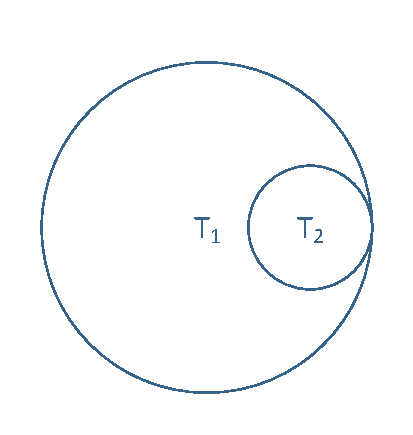
\includegraphics[width=1.31in]{testSuite1.eps}
}
\subfigure[]{
  %  \rule{4cm}{3cm}
    \label{fig:disjoint}
    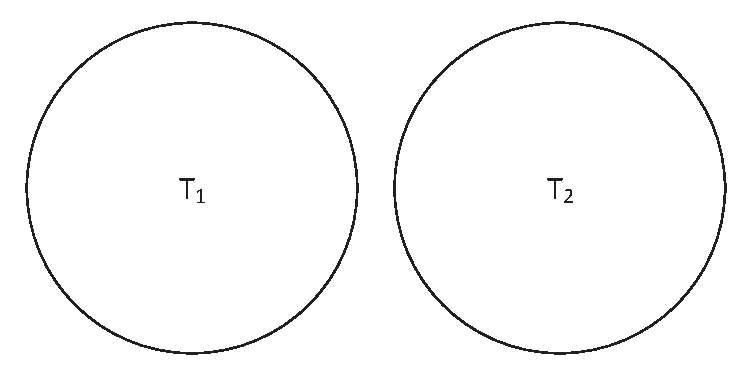
\includegraphics[width=2.01in]{testSuite2.eps}
}
\subfigure[]{
  %  \rule{4cm}{3cm}
    \label{fig:intersect}
    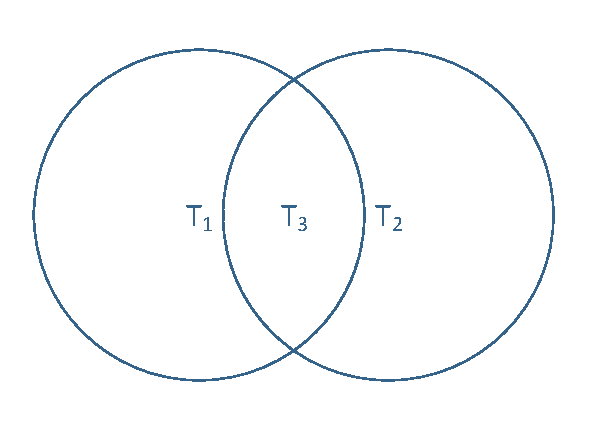
\includegraphics[width=1.81in]{testSuite3.eps}
}
\caption[]{Relationships between two test sets}
\label{fig:testSuite}
\end{figure*}

\subsection{Inclusion}

It is the first relationship corresponding to Figure \ref{fig:inclusion}. We have the following proposition for two test sets that have an inclusion relationship.
%\newtheorem{lemma}{Lemma}
\begin{proposition}[{schemas for test subset tend to be super schemas}]\label{pro:ssp}
For two sets of test cases $T_{l}$ and $T_{k}$, assume that $T_{l} \subset T_{k}$. Then $\forall c_{l} \in \mathcal{C}(T_{l})$, $\ either\ c_{l} \in \mathcal{C}(T_{k})\ or\ \exists c_{k} \in \mathcal{C}(T_{k}), s.t., c_{k} \prec c_{l}.$
\end{proposition}

\begin{proof}
Obviously $\forall c_{l} \in \mathcal{C}(T_{l})$,  $\mathcal{T}(c_{l}) \subset T_{l} \subset T_{k}$. According to Proposition \ref{pro:sbS}, $c_{l} \in \mathcal{S}(T_{k})$. So this proposition holds as the schema in $\mathcal{S}(T_{k})$ either is in $\mathcal{C}(T_{k})$, or must be the super-schemas of some schemas in $\mathcal{C}(T_{k})$.
\end{proof}

Likewise, we can get the properties of the schemas identified for the larger set of test cases.

\begin{proposition}[{schemas for test superset tend to be subschemas}]\label{pro:sls}
For two sets of test cases $T_{l}$ and $T_{k}$, assume that $T_{l} \subset T_{k}$. Then $\forall c_{k} \in \mathcal{C}(T_{k})\ $, it could be $\ (1)\ c_{k} \in \mathcal{C}(T_{l})\ $ , $(2)\ \exists c_{l} \in \mathcal{C}(T_{l}), s.t., c_{k} \prec c_{l}\ $ ,or $(3)\ \not\exists c_{l} \in \mathcal{C}(T_{l}), s.t., c_{k} \prec c_{l}\ or\ c_{k} = c_{l},\ or\ c_{l} \prec c_{k}.$
\end{proposition}

This proposition is exactly the antithesis of Proposition \ref{pro:ssp}. We need to note the third condition, i.e., $\ \not\exists c_{l} \in \mathcal{C}(T_{l}), s.t., c_{k} \prec c_{l}\ or\ c_{k} = c_{l},\ or\ c_{l} \prec c_{k}.$ We refer to this condition as $c_{k}$ is \emph{irrelevant} to $\mathcal{C}(T_{l})$. Furthermore, we can also say a schema is \emph{irrelevant} to another schema if these two schemas are neither identical nor subsuming each other.

We illustrate these scenarios in Table \ref{example_three_condition}. There are two parts in this table, with each part showing two sets of test cases: $T_{l}$ and $T_{k}$, which have $T_{l} \subset T_{k}$. In the left part, we can see that in the schema in $\mathcal{C}(T_{l})$: (0, 0, -) and (0, -, 0), both are the super-schemas of the one in $\mathcal{C}(T_{k})$:(0,-,-). While in the right part, the schemas in $\mathcal{C}(T_{l})$: (0, 0, -) and (0, -, 0) are both also in $\mathcal{C}(T_{k})$. Furthermore, one schema in $\mathcal{C}(T_{k})$: (1,1,-) is irrelevant to $\mathcal{C}(T_{l})$.

%in which the left part shows the case that the failure-inducing combinations satisfy the first properties( both (0,0,-) and (0,1,0) subsume (0,-,-)). While the right part give an example to the second properties, as (1,-,-) is irrelevant to any one of (0,0,-) and (0,1,0).

%\begin{proof}
%We proof this by two sides:
%
%for there is one failure-inducing combination is this set, then this condition is similar to proposition 1, and For there is multiple failure-inducing combinations. We can easily find it must exist one failure-inducing combination.
%\end{proof}

\begin{table}
\centering
\tbl{Inclusion example\label{example_three_condition}}{
  \begin{tabular}{cc}
$T_{l}$&$T_{k}$ \\ \hline
(0, 0, 0)&(0, 0, 0)\\
(0, 0, 1)&(0, 0, 1) \\
(0, 1, 0)&(0, 1, 0)\\
         &(0, 1, 1) \\ \hline
 $\mathcal{C}(T_{l})$& $\mathcal{C}(T_{k})$ \\ \hline
(0, 0, -)&(0, -, -)\\
(0, -, 0)&		   \\ \hline
  \end{tabular}
  \hspace{1em}
  \begin{tabular}{cc}
$T_{l}$&$T_{k}$\\ \hline
(0, 0, 0) & (0, 0, 0)\\
(0, 0, 1) & (0, 0, 1)\\
(0, 1, 0) & (0, 1, 0)\\
		  & (1, 1, 0)\\
		  & (1, 1, 1)\\ \hline
$\mathcal{C}(T_{l})$& $\mathcal{C}(T_{k})$ \\ \hline
(0, 0, -)&  (0, 0, -)\\
(0, -, 0)&  (0, -, 0)\\
		 &  (1, 1, -)\\  \hline
  \end{tabular}
  }
  \end{table}

%It is noted that as the

\subsection{Disjointness}
This relationship corresponds to Figure \ref{fig:disjoint}. For two different test sets, one obvious property is listed as follows:
\begin{proposition}[No relationships between the schemas]\label{pro:nrs}
 For two test sets $T_{1}$ and $T_{2}$, if $T_{1} \bigcap T_{2} = \emptyset $, we have, $\mathcal{S}(T_{1}) \bigcap \mathcal{S}(T_{2}) = \emptyset$.
\end{proposition}
\begin{proof}
 Assume that $\mathcal{S}(T_{1}) \bigcap \mathcal{S}(T_{2}) \ne \emptyset$. Without loss of generality, let $c \in \mathcal{S}(T_{1}) \bigcap \mathcal{S}(T_{2}) $, we can learn that $\mathcal{T}(c)$ must both in $T_{1}$ and $T_{2}$, which is contradiction.
\end{proof}

This property points out that the minimal schemas of two disjoint test cases should be irrelevant to each other. Table \ref{example_disjoint} shows an example of this scenario. We can learn from this table that for two different test sets $T_{l}$ and $T_{k}$, their minimal schemas, i.e., (0, - , 0) and (1, 0, -),(1, -, 0), respectively, are irrelevant to each other.
\begin{table}
\centering
\tbl{Disjoint example \label{example_disjoint}}{
  \begin{tabular}{cc}
$T_{l}$&$T_{k}$ \\ \hline
(0, 0, 0)&  (1, 0, 0)\\
(0, 1, 0)&  (1, 0, 1)\\
		 &  (1, 1, 0)\\  \hline
 $\mathcal{C}(T_{l})$& $\mathcal{C}(T_{k})$ \\ \hline
(0, -, 0)&(1, 0, -)\\
         &(1, -, 0)	\\ \hline
  \end{tabular}
  }
  \end{table}
%Sometimes they can be merged.

\subsection{Intersection}
This relationship corresponds to Figure \ref{fig:intersect}, which is the most common scenario for two given sets of test cases, but is also the most complicated scenario for analysis. To conveniently illustrate the properties of the minimal schemas for this scenario, let $T_{1} \bigcap T_{2} = T_{3}$ as depicted in Figure \ref{fig:intersect}. Then, to get the relationship between the schemas of $\mathcal{C}(T_{1})$ and $\mathcal{C}(T_{2})$, we need to use the intermediate schemas in $\mathcal{C}(T_{3})$.

As $T_{3} \subset T_{1}$, then according to Proposition \ref{pro:sls}, $\forall c_{1} \in \mathcal{C}(T_{1})$, we have $\exists c_{3} \in \mathcal{C}(T_{3})$, s.t. $c_{1} = c_{3} $ or, $c_{1} \prec c_{3}$, or $c_{1}$ irrelevant to $\mathcal{C}(T_{3})$.  Further, as $T_{3} \subset T_{2}$, then according to Proposition \ref{pro:ssp}, $\forall c_{3} \in \mathcal{C}(T_{3}) $, we have $\exists c_{2} \in \mathcal{C}(T_{2})$, s.t. $c_{2} = c_{3}$ or $c_{2} \prec c_{3}$. Combining these two properties, we can find the following possible scenarios for $c_{1},c_{3}$ and $c_{2}$ , as shown in Table \ref{possible-relation-of-intersection}. In this table, Column `$c_{1}\ and\ c_{3}$' shows the relationship between $c_{1}$ and $c_{3}$, Column `$c_{3}\ and\ c_{2}$' indicates the relationship between $c_{3}$ and $c_{2}$.
each row indicates a scenario in the form of $\forall c_{1} \in \mathcal{C}(T_{1}), \exists c_{3},\ s.t.,\ ...$ and correspondingly, $\exists c_{2} \in \mathcal{C}(T_{2}),\ s.t,\ ...$. For example, the first scenario means that $\forall c_{1} \in \mathcal{C}(T_{1}), \exists c_{3} \in \mathcal{C}(T_{3}),\ s.t.,\ c_{1} = c_{3}$ and correspondingly, $\exists c_{2} \in \mathcal{C}(T_{2}),\ s.t,\ c_{3} = c_{2}$. It is noted that for the 5th scenario, $c_{1}$ is irrelevant to $\mathcal{C}(T_{3})$, which means under this condition there is no single intermediate schema $c_{3}$. Hence, it is not necessary to list the relationship between $c_{3}$ and $c_{2}$, which is marked as `---'.


\begin{table}
\centering
  \begin{threeparttable}
\tbl{Possible scenarios for $c_{1}$, $c_{3}$ and $c_{2}$ \label{possible-relation-of-intersection}}{
  \begin{tabular}{c|c|c} \hline
id&$c_{1}$  and $c_{3}$  & $c_{3}$  and $c_{2}$  \\ \hline
1&$c_{1} = c_{3}$ & $c_{3} = c_{2}$ \\
2&$c_{1} = c_{3}$  & $c_{2} \prec c_{3}$ \\
3&$c_{1} \prec c_{3}$ & $c_{3} = c_{2}$ \\
4&$c_{1} \prec c_{3}$ & $c_{2} \prec c_{3}$ \\
5&$c_{1}\ irrelevant\ \mathcal{C}(T_{3})$ & --- \\ \hline
  \end{tabular}
  }
% \begin{tablenotes}
%        \footnotesize
%\item[\dag]$c_{1} \in \mathcal{C}(T_{1})$.
%\item[$\star$]$c_{2} \in \mathcal{C}(T_{2})$.
%\item[\S]$c_{3} \in \mathcal{C}(T_{3})$, $T_{3} = T_{1} \bigcap T_{2}$
%      \end{tablenotes}
  \end{threeparttable}
\end{table}

For each scenario in Table \ref{possible-relation-of-intersection}, a proposition will be given to describe the relationship between the corresponding schema $c_{1}$ and $c_{2}$.

\begin{proposition}[two identical]\label{pro:twoidentical}
$\forall c_{1} \in \mathcal{C}(T_{1})$ if $\exists c_{3} \in \mathcal{C}(T_{3}),\ s.t.,\ c_{3} = c_{1}$, and correspondingly, $\exists c_{2} \in \mathcal{C}(T_{2}),\ s.t.,\ c_{2} = c_{3}$. Then it must have $c_{1} = c_{2}$.
\end{proposition}

This proposition is obvious, and it indicates the minimal schemas for two intersect test sets can be identical.  For example, Table \ref{example_intersect_identical} shows two sets of test cases that interact with each other at test cases (1,1,0) and (1,1,1). It is easily found that the identical schema is (1,1,-) for $c_{1}$, $c_{2}$ and $c_{3}$. For the following proportions that are very obvious like Proposition \ref{pro:twoidentical}, we will omit the proof and just give an example to illustrate the corresponding proposition.

\begin{table}
\centering
\tbl{Example for scenario 1 \label{example_intersect_identical}}{
  \begin{tabular}{ccc}
$T_{1}$&$T_{2}$ &$T_{3} = T_{1} \bigcap T_{2}$\\ \hline
 (0, 1, 0) & (0, 0, 0) & (1, 1, 0) \\
 (1, 1, 0) & (0, 0, 1) & (1, 1, 1)\\
 (1, 1, 1) & (1, 1, 0) & \\
	       & (1, 1, 1) & \\\hline

 $\mathcal{C}(T_{1})$& $\mathcal{C}(T_{2})$ & $\mathcal{C}(T_{3})$  \\ \hline
(-, 1, 0)&  (0, 0, -) & (1, 1, -)\\
(1, 1, -)&  (1, 1, -) &\\ \hline
  \end{tabular}
  }
  \end{table}

\begin{proposition}[one identical, one sub]\label{pro:onesuboneidenticial}
$\forall c_{1} \in \mathcal{C}(T_{1})$ if $\exists c_{3} \in \mathcal{C}(T_{3}),\ s.t.,\ c_{3} = c_{1}$, and correspondingly, $\exists c_{2} \in \mathcal{C}(T_{2}),\ s.t.,\ c_{2} \prec c_{3}$. Then it must have $c_{2} \prec c_{1}$.
\end{proposition}

Table \ref{example_intersect_subsume} illustrates this scenario. We can find that the minimal schemas for $T_{1}$: (1,0,-),(1,-,0) are identical to the schemas in $\mathcal{C}(T_{3})$, which are the super schemas of the minimal schema for $T_{2}$: (1,-,-).

\begin{table}
\centering
\tbl{Example for scenario 2 \label{example_intersect_subsume}}{
  \begin{tabular}{ccc}
$T_{1}$&$T_{2}$ &$T_{3}  = T_{1} \bigcap T_{2} $\\ \hline
(0, 1, 0)   & (0, 0, 0) & (1, 0, 0) \\
(1, 0, 0)   & (1, 0, 0) & (1, 0, 1)\\
(1, 0, 1)	& (1, 0, 1) & (1, 1, 0)\\
(1, 1, 0)	& (1, 1, 0) &         \\
        	& (1, 1, 1) & \\ \hline
 $\mathcal{C}(T_{1})$& $\mathcal{C}(T_{2})$ & $\mathcal{C}(T_{3})$  \\ \hline
(-, 1, 0)&  (-, 0, 0) & (1, 0, -)\\
(1, 0, -)&  (1, -, -) & (1, -, 0)   \\
(1, -, 0)&     & \\ \hline
  \end{tabular}
  }
  \end{table}



\begin{proposition}[one sub, one identical]\label{pro:oneidenticalonesub}
$\forall c_{1} \in \mathcal{C}(T_{1})$ if $\exists c_{3} \in \mathcal{C}(T_{3}),\ s.t.,\ c_{1} \prec c_{3}$, and correspondingly, $\exists c_{2} \in \mathcal{C}(T_{2}),\ s.t.,\ c_{2} = c_{3}$. Then it must have $c_{1} \prec c_{2}$.
\end{proposition}

This proposition is exactly the antithesis of Proposition \ref{pro:onesuboneidenticial}. An example of this scenario can be easily obtained by transforming the label $T_{1}$ to $T_{2}$, and $T_{2}$ to $T_{1}$ in Table \ref{example_intersect_subsume}.


\begin{proposition}[two sub]\label{pro:twosub}
$\forall c_{1} \in \mathcal{C}(T_{1})$ if $\exists c_{3} \in \mathcal{C}(T_{3}),\ s.t.,\ c_{1} \prec c_{3}$, and correspondingly, $\exists c_{2} \in \mathcal{C}(T_{2}),\ s.t.,\ c_{2} \prec c_{3}$.Then it must have $c_{1}$ is irrelevant to $c_{2}$.
\end{proposition}
\begin{proof}
First we have $\mathcal{T}(c_{1}) \not\subset  T_{3}$. This is because if not so, according to Proposition \ref{pro:ssp} it has $\exists c_{3}' \in \mathcal{C}(T_{3}),\ s.t.,\ c_{3}' \prec c_{1},\ or\ c_{3}' = c_{1}$. Then as $\exists c_{3} \in \mathcal{C}(T_{3}),\ s.t.,\ c_{1} \prec c_{3}$, based on which it has $c_{3}' \prec c_{3}$. This is not possible as both $c_{3}', c_{3} \in \mathcal{C}(T_{3})$, which means that they are both minimal schemas. So $\mathcal{T}(c_{1}) \not\subset  T_{3}$ holds.

Based on this, there must exist at least one test case $t \in \mathcal{T}(c_{1})$, such that $t \not\in T_{3}$. As $\mathcal{T}(c_{1}) \subset T_{1}$, then the corresponding test case $t$ must belong to $T_{1} \backslash T_{3}$. Formally, $\exists t \in \mathcal{T}(c_{1}),\ s.t.,\ t \in T_{1} \backslash T_{3}$.

Similarly, it also has $\exists t \in \mathcal{T}(c_{2}),\ s.t.,\ t \in T_{2} \backslash T_{3}$.

As $T_{2} \backslash T_{3} \bigcap T_{1} \backslash T_{3} = \varnothing$, then $\exists t \in \mathcal{T}(c_{1}),\ s.t.,\ t \not\in \mathcal{T}(c_{2})$ and $\exists t \in \mathcal{T}(c_{3}),\ s.t.,\ t \not\in \mathcal{T}(c_{1})$. Consequently, we have $\mathcal{T}(c_{1}) \not\subset \mathcal{T}(c_{2})$, $\mathcal{T}(c_{2}) \not\subset \mathcal{T}(c_{1})$, and  $\mathcal{T}(c_{1}) \neq \mathcal{T}(c_{2})$. Hence, $c_{2} \not\prec c_{1}$, $c_{1} \not\prec c_{2}$ and $c_{1} \neq c_{2}$, which indicates that $c_{1}$ is irrelevant to $c_{2}$.
\end{proof}


Note that under this condition we can only determine that schema $c_{1}$ and $c_{2}$ are irrelevant, it may happen that $c_{1}$ is related to other schema in $\mathcal{C}(T_{2})$.  Under this condition, assume $c_{2}' \in \mathcal{C}(T_{2})$ is related to $c_{1}$. In fact, the only relationship between $c_{1}$ and $c_{2}'$ is $c_{1} \prec c_{2}'$.  This is because we have proved that $\exists t \in \mathcal{T}(c_{1}),\ s.t.,\ t \not\in \mathcal{T}(c_{2})$, which means that $\mathcal{T}(c_{1}) \not\subset \mathcal{T}(c_{2}')$ and  $\mathcal{T}(c_{1}) \neq \mathcal{T}(c_{2}')$. Hence $\forall c_{2}' \in \mathcal{C}(T_{2}),  c_{1} \neq c_{2}' \ and\ c_{2}' \not\prec c_{1}$. So the only possible relationships between $c_{1}$ and other schemas in $\mathcal{C}(T_{2})$ are either irrelevant or $\exists c_{2}' \in \mathcal{C}(T_{2}),\ s.t.,\ c_{1} \prec c_{2}'$. Formally, we can describe the relationships between $c_{1}$ and $\mathcal{C}(T_{2})$ in Lemma \ref{lemma:twosub}.
%\newtheorem{lemma}{Lemma}
%\begin{lemma}
\begin{lemma}[two sub]\label{lemma:twosub}
$\forall c_{1} \in \mathcal{C}(T_{1})$ if $\exists c_{3} \in \mathcal{C}(T_{3}),\ s.t.,\ c_{1} \prec c_{3}$, and correspondingly, $\exists c_{2} \in \mathcal{C}(T_{2}),\ s.t.,\ c_{2} \prec c_{3}$. Then it must have either $c_{1}\ is\ irrelevant\ to\ \mathcal{C}(T_{2}),\ or\ \exists c_{2}' \in \mathcal{C}(T_{2}),\ s.t.,\ c_{1} \prec c_{2}'$.
\end{lemma}


Table \ref{example_intersect_subsub} gives an example for the two possible relationships between $c_{1}$ and $\mathcal{C}(T_{2})$. In the left main column, we can find that $c_{1}$ $(-,-,0)$ and $c_{2}$ $(1,-,-)$ are both the sub schema of $c_{3}$ $(1,-,0)$, and they are irrelevant to each other.  Further, as there is no extra minimal schemas in $\mathcal{C}(T_{2})$, so $c_{1}$ is irrelevant to $\mathcal{C}(T_{2})$.  In the right column,  $c_{1}$ $(-,-,1)$ and $c_{2}$ $(1,1,-)$ are both the sub schema of $c_{3}$ $(1,-,0)$ , and they are still irrelevant to each other. But $c_{1}$ is the sub schema of $c_{2}'$ (0,0,1), which is also the minimal schema in $\mathcal{C}(T_{2})$.

\begin{table}
\centering
\tbl{Example for scenario 4  \label{example_intersect_subsub}}{
  \begin{tabular}{ccc}
$T_{1}$&$T_{2}$ &$T_{3}  = T_{1} \bigcap T_{2} $\\ \hline
(0, 0, 0)   & (1, 0, 0) & (1, 0, 0) \\
(0, 1, 0)   & (1, 0, 1) & (1, 1, 0)\\
(1, 0, 0)	& (1, 1, 0) &  \\
(1, 1, 0)	& (1, 1, 1) &         \\ \hline
 $\mathcal{C}(T_{1})$& $\mathcal{C}(T_{2})$ & $\mathcal{C}(T_{3})$  \\ \hline
(-, -, 0)&  (1, -, -) & (1, -, 0)\\ \hline
%         &  (-, 0, 1) &  \\
  \end{tabular}
  \hspace{1em}
  \begin{tabular}{ccc}
$T_{1}$&$T_{2}$ &$T_{3}  = T_{1} \bigcap T_{2} $\\ \hline
(0, 0, 1)   & (0, 0, 1)       & (0, 0, 1) \\
(0, 1, 1)   & (1, 1, 1)       & (1, 1, 1)\\
(1, 0, 1)	& (1, 1, 0)       &           \\
(1, 1, 1)	&   &         \\ \hline
 $\mathcal{C}(T_{1})$& $\mathcal{C}(T_{2})$ & $\mathcal{C}(T_{3})$  \\ \hline
 (- ,-, 1)  &  (0, 0, 1) & (0, 0, 1)\\
            &  (1, 1, -) & (1, 1, 1) \\  \hline
  \end{tabular}
  }
  \end{table}

\begin{proposition}[one irrelevant]\label{pro:oneirrelevant}
For $c_{1} \in \mathcal{C}(T_{1})$, if $c_{1}\ irrelevant\ to\ \mathcal{C}(T_{3})$. Then it must have $c_{1}\ irrelevant\ to\ \mathcal{C}(T_{2})$
\end{proposition}

\begin{proof}
Assume $c_{1}$ is related to $\mathcal{C}(T_{2})$, i.e., $\exists c_{2} \in \mathcal{C}(T_{2}),\ s.t.,\ c_{1} \prec c_{2},\ or\ c_{2} \prec c_{1},\ or\ c_{1} = c_{2}$.

For the first case, i.e., if $c_{1} \prec c_{2}$, it then must have $\mathcal{T}(c_{2}) \subset \mathcal{T}(c_{1})$ according to Proposition \ref{pro:shl}.  Further it have $\mathcal{T}(c_{2}) \subset T_{3}$, because if not so, then $\exists t \in \mathcal{T}(c_{2}),\ s.t.,\ t \in T_{2} \backslash T_{3}$. As $T_{2} \backslash T_{3} \bigcap T_{1} = \varnothing $, then $\exists t \in \mathcal{T}(c_{2}),\ s.t.,\ t \not\in T_{1}$. As $\mathcal{T}(c_{1}) \subset T_{1}$, then $\exists t \in \mathcal{T}(c_{2}),\ s.t.,\ t \not\in \mathcal{T}(c_{1})$, which means that $\mathcal{T}(c_{2}) \not\subset \mathcal{T}(c_{1})$.  It is contradiction, so $\mathcal{T}(c_{2}) \subset T_{3}$.

Then according to Proposition \ref{pro:ssp},  $\exists c_{3} \in \mathcal{C}(T_{3}),\ s.t.\ c_{3} \prec c_{2}\ or\ c_{3} = c_{2}$. Note that $c_{2} \in \mathcal{C}(T_{2})$ and $T_{3} \subset T_{2}$, then according to Proposition \ref{pro:sls},  $\exists c_{3} \in \mathcal{C}(T_{3}),\ s.t.,\ c_{2} \prec c_{3},\ or\ c_{2} = c_{3},\ or\ c_{2}\ is\ irrelevant\ to\ \mathcal{C}(T_{3})$. Combining these two properties, it can only happen $\exists c_{3} \in \mathcal{C}(T_{3}),\ s.t.,\ c_{2} = c_{3}$.
As $c_{1} \prec c_{2}$, then we can have $\exists c_{3} \in \mathcal{C}(T_{3}), s.t., c_{1} \prec  c_{3}$. It is contradiction as $c_{1}\ irrelevant\ to\ \mathcal{C}(T_{3})$. So the first case is impossible, which indicates that $c_{1} \not\prec c_{2}$.


For the second case, i.e., if $c_{2} \prec c_{1}$. Then it must have $\mathcal{T}(c_{1}) \subset \mathcal{T}(c_{2})$. Similarly as the first case, we further have $\mathcal{T}(c_{1}) \subset T_{3}$. Then according to Proposition \ref{pro:ssp}, $\exists c_{3} \in  \mathcal{C}(T_{3}),\ s.t.\ c_{3} \prec c_{1}\ or\ c_{3} = c_{1}$. It is also contradiction to the fact that $c_{1}\ irrelevant\ to\ \mathcal{C}(T_{3})$. So the second case is not possible, which indicates that  $c_{2} \not\prec c_{1}$.


For the last case, i.e., if $c_{1} = c_{2}$. Then it must have $\mathcal{T}(c_{2}) = \mathcal{T}(c_{1})$. Further we have $\mathcal{T}(c_{1}) \subset T_{3}$. Because if not so, then $\exists t \in \mathcal{T}(c_{1}),\ s.t.,\ t \in T_{1} \backslash T_{3}$. As $T_{1} \backslash T_{3} \bigcap T_{2} = \varnothing $, then $\exists t \in \mathcal{T}(c_{1}),\ s.t.,\ t \not\in T_{2}$. As $\mathcal{T}(c_{2}) \subset T_{2}$, so  $\exists t \in \mathcal{T}(c_{1}),\ s.t.,\ t \not\in \mathcal{T}(c_{2})$, indicating that $\mathcal{T}(c_{1}) \neq \mathcal{T}(c_{2})$. It is contradiction, so $\mathcal{T}(c_{1}) \subset T_{3}$.

Then as $\mathcal{T}(c_{1}) \subset T_{3}$, according to Proposition \ref{pro:ssp}, $\exists c_{3} \in  \mathcal{C}(T_{3}),\ s.t.\ c_{3} \prec c_{1}\ or\ c_{3} = c_{1}$. It is still contradiction to the fact that $c_{1}\ irrelevant\ to\ \mathcal{C}(T_{3})$. So the last case is not possible, which indicates that $c_{1} \neq c_{2}$.

As all these three cases are impossible, so $c_{1}$ is must irrelevant to $\mathcal{C}(T_{2})$.
\end{proof}

For example, in Table \ref{example_intersect_irrelevant}, schema $c_{1}$ $(0,1,-)$  is irrelevant to $\mathcal{C}(T_{3})$, i.e., \{ $(1,-,0)$ \}. It can be found that $c_{1}$ $(0,1,-)$ is also irrelevant to $\mathcal{C}(T_{2})$, i.e., \{ $(1,-,-)$ , $(-,0,1)$ \}.

\begin{table}
\centering
\tbl{Example for scenario 5 \label{example_intersect_irrelevant}}{
  \begin{tabular}{ccc}
$T_{1}$&$T_{2}$ &$T_{3}  = T_{1} \bigcap T_{2} $\\ \hline
(0, 0, 0)   & (1, 0, 0) & (1, 0, 0) \\
(0, 1, 0)   & (1, 0, 1) & (1, 1, 0)\\
(1, 0, 0)	& (1, 1, 0) &  \\
(1, 1, 0)	& (1, 1, 1) &         \\
(0, 1, 1)   & (0 ,0,1)  &  \\ \hline
 $\mathcal{C}(T_{1})$& $\mathcal{C}(T_{2})$ & $\mathcal{C}(T_{3})$  \\ \hline
(-, -, 0)&  (1, -, -) & (1, -, 0)\\
(0,1 , -) &  (-, 0, 1) &  \\  \hline
  \end{tabular}
  }
  \end{table}


%It is noted that this proposition holds when some schemas in $\mathcal{C}(T_{3})$ are also in $\mathcal{C}(T_{1})$ (or $\mathcal{C}(T_{2})$), and simultaneously the same schemas in $\mathcal{C}(T_{3})$ must be the super-schema of the minimal schemas of another set of test cases, i.e., $\mathcal{C}(T_{2})$ (or $\mathcal{C}(T_{1})$).

%It is noted that these three conditions can simultaneously appear when two sets of test cases intersect with each other.

Table \ref{possible-result-of-intersection} concludes the possible relationships between $c_{1}$ and $\mathcal{C}(T_{2})$ under the previous five scenarios. The three columns in the left are the same as Table \ref{possible-relation-of-intersection}. The last column ` $c_{1}$ and $\mathcal{C}(T_{2})$' indicates the relationship between schema $c_{1}$ and $\mathcal{C}(T_{2})$. From this table, we can learn that for two intersect sets of test cases, i.e., $T_{1}$ and $T_{2}$, there are four possible relationships between a schema $c_{1} \in  \mathcal{C}(T_{1})$ and $\mathcal{C}(T_{2})$. Formally, we have the following proposition.

\begin{proposition}[conclusion for intersection]\label{pro:concludeforintersection}
$\forall c_{1} \in \mathcal{C}(T_{1}), \exists c_{2} \in  \mathcal{C}(T_{1}),\ s.t.,\ (1)\ c_{1} = c_{2}\ (scenario 1), \ or\ (2)\ c_{2} \prec c_{1}\ (scenario 2),\ or\ (3)\ c_{1} \prec c_{2}\ (scenario 3, scenario 4),\ or\ (4)\ c_{1}\ is\ irrelevant\ to\ \mathcal{C}(T_{2})\ (scenario 5, scenario 4).$
\end{proposition}

%Note that the 4th scenario (marked $\star$) only shows that two corresponding schema $c_{1}$ and $c_{2}$ are irrelevant. It may happen that $c_{1}$ is related to other schemas in $\mathcal{C}(T_{2})$.  Under this condition, assume $c_{2}' \in \mathcal{C}(T_{2})$ is related to $c_{1}$. In fact, the only relationship between $c_{1}$ and $c_{2}'$ is that $c_{1} \prec c_{2}$ because
%which may be transformed to scenario 3; or $c_{1}$ will be irrelevant to all the other schemas in $\mathcal{C}(T_{2})$, which will be transformed to scenario 5.

%their minimal schemas can be identical (scenario 1),  can be subsuming each other (scenarios 2 and 3), can be irrelevant to each other (scenario 4),  and can be irrelevant to all the minimal schemas of the other set of test cases (scenario 5).

\begin{table}
\centering
\tbl{Possible relationships between $c_{1}$ and $\mathcal{C}(T_{2})$  \label{possible-result-of-intersection}}{
  \begin{tabular}{c|c|c||c} \hline
id&$c_{1}$ and $c_{3}$ & $c_{2}$ and $c_{3}$  & $c_{1}$ and $\mathcal{C}(T_{2})$\\ \hline
1&$c_{1} = c_{3}$ & $c_{3} = c_{2}$  & $c_{1} =  c_{2}$\\
2&$c_{1} = c_{3}$  & $c_{2} \prec c_{3}$ &  $c_{2} \prec c_{1}$ \\
3&$c_{1} \prec c_{3}$ & $c_{3} = c_{2}$ & $c_{1} \prec c_{2}$ \\
4&$c_{1} \prec c_{3}$ & $c_{3} \prec c_{2}$ &  $c_{1}$ irrelevant to $\mathcal{C}(T_{2})$, or $\exists c_{2}' \in \mathcal{C}(T_{2}),\ s.t.,\ c_{1} \prec c_{2}'$ \\
5&$c_{1}\ irrelevant\ \mathcal{C}(T_{3})$ & --- & $c_{1}$ irrelevant to $\mathcal{C}(T_{2})$  \\ \hline
  \end{tabular}
  }
  \end{table}

%\subsection{Summary of the formal model}
%From the previous analysis, we can learn that for the general intersect test cases-schema model, this is a partial relationship.

\subsection{Identify the MFS}
According to Definition \ref{de:mfs} and Proposition \ref{pro:ash}, we can determine that $\mathcal{C}(T_{F_{m}})$ actually is the set of failure-causing schemas of $F_{m}$. Then in theory, if we want to accurately figure out the MFS in the SUT, we need to exhaustively execute each possible test case, and collect the failing test cases $T_{F_{m}}$. This is impossible in practice, especially when the testing space is very large.

Traditional FCI approaches select a subset of the exhaustive test cases to execute. In this case, in order to identify the MFS, each of the remaining test cases must be predicted to be failing or not. Or alternatively, a set of schemas is given as the candidate of the MFS \cite{ghandehari2012identifying}. For this case, these schemas should be ranked according to their likelihood to be the MFS. As giving a ranking of these candidate schemas can also be regard as a special case of making a prediction (with computing the probability), so we next only formally describe the mechanism of FCI approaches for the first case.

%This prediction is based on some assumptions and not always correct. Formally, we can describe the two ways as following:
We refer to the observed failing test case as  $T_{fail_{observed}}$, and the remaining failing test cases based on prediction as $T_{fail_{predicted}}$. We also denote the actual entire failing test cases as $T_{fail}$. Then the MFS identified by FCI approaches can be depicted as:

MFS = $\mathcal{C}(T_{fail_{observed}} \bigcup T_{fail_{predicted}})$.

Each FCI approach applies different way to predict $T_{fail_{predicted}}$ according to observed failing test cases; furthermore, as test cases generated are different, the failing test cases observed by different FCI approaches, i.e., $T_{fail_{observed}}$ also vary.

We offer an example using the OFOT approach \cite{nie2011minimal} to identify the MFS. Suppose that the SUT has 3 parameters, each of which can take on 2 values, and assume the test case (1, 1, 1) failed. Then, the FCI process using OFOT approach can be illustrated in Table \ref{ofot-identify}. In this table, test case \emph{t} failed, and OFOT mutated one parameter value of test case \emph{t} at a time to generate new test cases: $t_{1}; t_{2}; t_{3}$. The pass of $t_{1}$ indicates that this test case breaks the MFS in the original test case \emph{t}. So, (1,-,-) should be one failure-causing factor, and as the other test cases ($t_{2}, t_{3}$) all failed , this means no other failure-inducing factors were broken; therefore, the MFS in \emph{t} is (1,-,-).

Now let us explain this process with our formal model. Obviously $T_{fail_{observed}}$ is \{(1,1,1),(1,0,1),(1,1,0)\}. And as (0,-,-) broke the MFS, by theory \cite{nie2011minimal}, all the test cases that contain (0,-,-) should pass the testing (This conclusion is built on the assumption that the SUT just contains one failure-causing schema).  As a result, {(0,1,1),(0,0,1),(0,1,0),(0,0,0)} should pass the testing. Further, as obviously the test case either passes or fails (the condition that a test case skips testing, i.e., does not produce an output, is labeled as a special case of failing), so the remaining test case (1,0,0), will be predicted to be failing, i.e., $T_{fail_{predicted}}$ is \{(1,0,0)\}. Finally, the MFS from the OFOT strategy can be described as: $\mathcal{C}(T_{fail_{observed}} \bigcup T_{fail_{predicted}})$ = $\mathcal{C}(\{(1,1,1),(1,0,1),(1,1,0),(1,0,0)\})$ = (1,-,-), which is identical to the one obtained previously.

\begin{table}[h]
\tbl{OFOT with our strategy\label{ofot-identify}}{
\begin{tabular}{llllll}
\multicolumn{5}{c}{\bfseries original test case} & \bfseries Outcome \\ \hline
 $t$ & \multicolumn{4}{l}{1 \ \ \ \ 1 \ \ \ \  1 } & Fail \\
 \hline
\multicolumn{5}{c}{\bfseries observed} &  \\ \hline
$t_{1}$ &\multicolumn{4}{l}{0  \ \ \ \  1 \ \ \ \  1 }& Pass \\
$t_{2}$ &\multicolumn{4}{l}{1  \ \ \ \  0 \ \ \ \  1 } & Fail \\
$t_{3}$ &\multicolumn{4}{l}{1  \ \ \ \  1 \ \ \ \  0 } & Fail \\
\hline
\multicolumn{5}{c}{\bfseries predicted} & \\ \hline
$t_{4}$ &\multicolumn{4}{l}{0  \ \ \ \  0 \ \ \ \  1 } & Pass \\
$t_{5}$ &\multicolumn{4}{l}{0  \ \ \ \  1 \ \ \ \  0 } & Pass \\
$t_{6}$ &\multicolumn{4}{l}{1  \ \ \ \  0 \ \ \ \  0 } & Fail \\
$t_{7}$ &\multicolumn{4}{l}{0  \ \ \ \  0 \ \ \ \  0 } & Pass \\ \hline
\end{tabular}}
\end{table}
%In this formula, the approach can derive the $T_{fail_{assumed}}$ from the $T_{fail_{observed}}$. For example,  for OFOT, one factor, pass, it can learn all the factor. For colbourn, it can learn from the covering array to be all according the number and t.



Similarly, other FCI approaches can also be modeled using this formal description. It is noted that the test cases FCI predicts to be failing are not always identical to the actually failing test cases. In fact, a more general scenario for FCI approaches can be depicted as shown in Figure \ref{fig:fci_process}.

\begin{figure}[h]
\centering
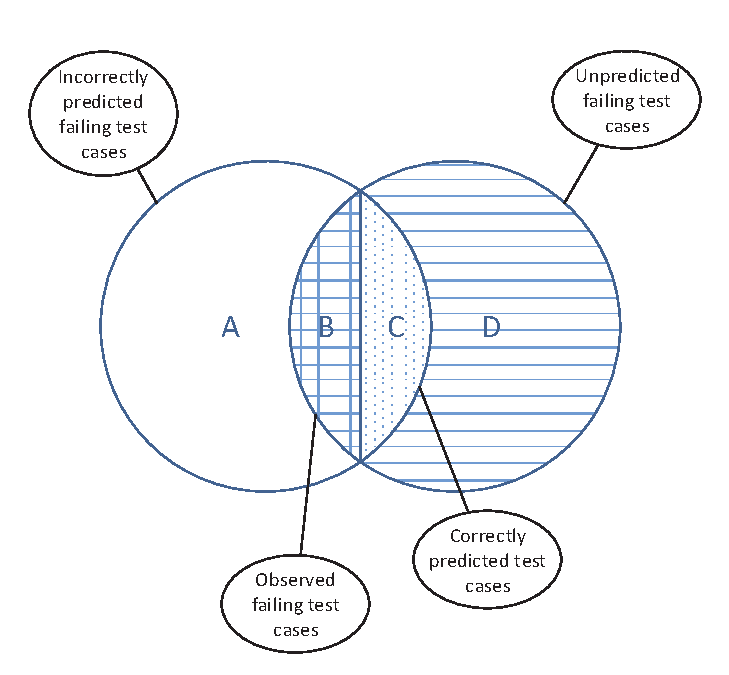
\includegraphics[width=4.31in]{FCI.eps}
\caption{A general model of FCI approach}
\label{fig:fci_process}
\end{figure}


In Figure \ref{fig:fci_process} area A denotes the test cases that should have passed testing but were predicted to be failing, area B depicts the test cases that the approach observed to be failing test cases, area C refers to the failing test cases that were not observed but were predicted to be failing test cases, and area D shows the failing test cases that are neither observed nor predicted.  This figure actually represents the condition in which two sets of test cases intersect with each other; specifically, comparing to the Figure \ref{fig:intersect}, we can learn that $A \bigcup B \bigcup C $= $T_{1}$, which indicates the test cases we think they are failing test cases.
 $D \bigcup B \bigcup C $= $T_{2}$  are the actual failing test cases,
and $ B \bigcup C$ = $ T_{1} \bigcap T_{2} = T_{3}$ are their Intersections.

%As we have known, in the case of Figure \ref{fig:intersect}, there are various relationships between the schemas identified in $T_{1}$ and the schemas identified in $T_{2}$.

According to the Proposition \ref{pro:concludeforintersection}, $\forall c_{1} \in \mathcal{C}(A \bigcup B \bigcup C),\ \exists c_{2} \in \mathcal{C}(D \bigcup B \bigcup C),\ s.t., \ (1)\ c_{1} = c_{2}\ , \ or\ (2)\ c_{2} \prec c_{1}\ ,\ or\ (3)\ c_{1} \prec c_{2}\ ,\ or\ (4)\ c_{1}\ is\ irrelevant\ to\ \mathcal{C}(T_{2})\ .$ This indicates that the identified minimal schema can be identical to some actual MFS, or be super-schema, or be sub schema, or be irrelevant to all the actual MFS.  Similarly, we can get the actual MFS can be identical to some identified schema, or be super-schema, or be sub schema, or be irrelevant to all the identified schemas. We refer to the case that the actual MFS is irrelevant to all the identified schemas as \emph{ignoring} the actual MFS.

%and in $\mathcal{C}(T_{2})$ must be irrelevant to each other. Mapping to Figure \ref{fig:fci_process}, we can get that some schemas in $\mathcal{C}(A \bigcup B \bigcup C)$ and in $\mathcal{C}(D \bigcup B \bigcup C)$ must be irrelevant to each other, which means that the FCI approach will identify some minimal schemas that are irrelevant to the actual MFS, and must ignore some actual MFS. Moreover, under the appropriate conditions listed in Propositions \ref{pro:ci} and \ref{pro:cs}, FCI may identify the identical schemas or super-schema or sub-schema of the actual MFS. In this case, the schemas (identical ones, super-schemas, or sub-schemas) are all depended on the area $B \bigcup C$, namely $T_{1} \bigcap T_{2}$ in Figure \ref{fig:intersect}.

To identify the schemas as accurately as possible, the FCI approach needs to make $A \bigcup B \bigcup C$ as similar as possible to $D \bigcup B \bigcup C$.

However, even though each FCI approach tries to identify the MFS as accurately as possible, masking effects arising from different test cases will reduce its effectiveness. We next discuss the masking problem and how it affects the FCI approaches.


\section{Masking effect}
\begin{definition}
A \emph{masking effect} occurs when a test case \emph{t} contains an MFS for a particular failure, but it does not trigger the expected failure because another failure was triggered ahead of it that prevents $t$ from being normally checked.
\end{definition}

Taking the masking effects into account, when identifying the MFS for a specific failure, say, $F_{m}$, we should not ignore those test cases which did not trigger $F_{m}$ but should have triggered it. We call these test cases $T_{mask(F_{m})}$. Hence, the MFS for failure $F_{m}$ should be $\mathcal{C}(T_{F_{m}} \bigcup T_{mask(F_{m})})$.

As an example, in the motivation example in section 2, $F_{mask(F_{Ex\ 2})}$  is \{ (7,4,4,5),(11,4,4,5)\}, So the MFS for $Ex 2$ is $\mathcal{C}(T_{F_{Ex\ 2}} \bigcup T_{mask(F_{Ex\ 2})})$, which is (-,-,4,5).

In practice with masking effects, however, it is not possible to correctly identifying the MFS, unless we fix some bugs in the SUT and re-execute the test cases to figure out $T_{mask(F_{m})}$.

For traditional FCI approaches, without the knowledge of  $T_{mask(F_{m})}$,  two common strategies can be adopted when facing the multiple failures problem, i.e., \emph{regarded as one failure}  and \emph{distinguishing failures}.  The former strategy treats all types of failures as one failure--\emph{failure}, and others as \emph{pass}, while the latter distinguishes the failures but with no special consideration of the masking effects, i.e., if a test case fails with a particular type of fault, this strategy presumes it does not contain other type of faults. We will separately discuss the two strategies under exhaustive testing condition and normal FCI testing condition.
\subsection{Masking effects under exhaustive testing}

\subsubsection{Regarded as one failure strategy}
%, as it does not distinguish the failures, i.e., it treats all types of failures as one failure--\emph{failure}, and others as \emph{pass}.
This is the most common strategy. With this strategy, the minimal schemas are the set $\mathcal{C}(\bigcup_{i = 1}^{L}T_{F_{i}})$ , $L$ is the number of all the failures in the SUT. Obviously, $T_{F_{m}} \bigcup T_{mask(F_{m})} \subset \bigcup_{i = 1}^{L}T_{F_{i}}$ . So in this case, by Proposition \ref{pro:sls}, some schemas obtained may be the sub-schemas of some of the actual MFS, or be irrelevant to the actual MFS.

As an example, consider the test cases in Table \ref{masking-effects-exhaustive}. Assume we need to characterize the MFS for error \emph{1}. All the test cases that triggered $Err_{1}$ are listed in column \emph{$T_{Err_{1}}$}; similarly, we list the test cases that triggered other failures in column \emph{$T_{mask(Err_{1})}$} and \emph{$T_{non\_mask}$}, respectively, in which the former masked $Err_{1}$, while the latter did not. Actually the MFS for $Err_{1}$  should be (1,1,-,-) and (-,1,1,1) as we listed them in the column \emph{actual MFS for 1}. However, when we use the \emph{regarded as one failure} strategy, the minimal schemas obtained will be (-,-,0,0), (1,1,-,-), (-,-,1,1), in which (-,-,0,0) is irrelevant to the actual MFS for $Err_{1}$ , and (-,-,1,1) is a sub-schema of the actual MFS (-,1,1,1).

\begin{table}
\centering
\tbl{masking effects for exhaustive testing \label{masking-effects-exhaustive}}{
  \begin{tabular}{ccc}
$T_{Err_{1}}$&$T_{mask(Err_{1})}$ &$T_{non\_mask}$\\ \hline
(1, 1, 1, 1)& (1, 1, 0, 0) & (0, 1, 0, 0) \\
(1, 1, 1, 0)& (0, 1, 1, 1) & (0, 0, 0, 0)\\
(1, 1, 0, 1)&              & (1, 0, 0, 0)\\
          	&              & (1, 0, 1, 1)\\
        	&              & (0, 0, 1, 1)\\ \hline
actual MFS for Err1&  regarded as one failure & distinguishing failures  \\
$\mathcal{C}(T_{Err_{1}} \bigcup T_{mask(Err_{1})})$& $\mathcal{C}( T_{Err_{1}} \bigcup T_{mask(Err_{1})}  \bigcup T_{non\_mask})$ & $\mathcal{C}(T_{Err_{1}})$  \\ \hline
(1, 1, -, -)&  (-, -, 0, 0) & (1, 1, -, 1)\\
(-, 1, 1, 1)&  (1, 1, -, -) & (1, 1, 1, -)   \\
            &  (-, -, 1, 1) &         \\ \hline
  \end{tabular}
  }
  \end{table}

\subsubsection{Distinguishing failures strategy}
Distinguishing the failures by the exception traces or error code can help identify the MFS related to particular failure. Yilmaz \cite{yilmaz2013reducing} proposed the \emph{multiple-class} failure characterizing method instead of the \emph{ternary-class} approach to make the characterizing process more accurate. Besides, other approaches can also be easily extended with this strategy for testing SUT with multiple failures.
%We call this strategy \emph{distinguishing failures}.

This strategy focuses on identifying the set of $\mathcal{C}(T_{F_{m}})$. As $T_{F_{m}} \bigcup T_{mask(F_{m})} \supset T_{F_{m}} $, some schemas obtained by this strategy may be the super-schema of some actual MFS. Moreover, some MFS may be irrelevant to the schemas obtained by this strategy, which means this strategy will \emph{ignore} these actual MFS.

For the simple example shown in Table \ref{masking-effects-exhaustive}, when using this strategy, we will get the minimal schemas (1, 1, -, 1) and (1, 1, 1, -), which are both super schemas of the actual MFS (1,1,-,-). Furthermore, no schemas obtained by this strategy have any relationship with the actual MFS (-,1,1,1), which means it was ignored.

It is noted that the motivation example in section 2 actually adopted this strategy. As a result, the schemas identified for Ex 2: (-,2,4,5), (-,3,4,5) are the super-schemas of the correct MFS(-,-,4,5).

\subsection{Masking effects under FCI approaches}
With masking effects, the scenario of traditional FCI approaches is a bit more complicated than the previous two exhaustive testing scenarios, and is depicted in Figure \ref{fig:fci_mask}. In this figure,  areas A, C and D are the same as those in Figure \ref{fig:fci_process}, and area B is further divided into three sub-areas in which $B_{1}$ still represents the observed failing test cases for the current analysed failure, area $B_{2}$ represents the test cases that triggered other failures which masked the current failure, and area $B_{3}$ represents the test cases that triggered other failures which did not mask the current failure. It can be found that the actual MFS set for the SUT is $\mathcal{C}(B_{1} \bigcup B_{2} \bigcup C \bigcup D)$.

\begin{figure}
\centering
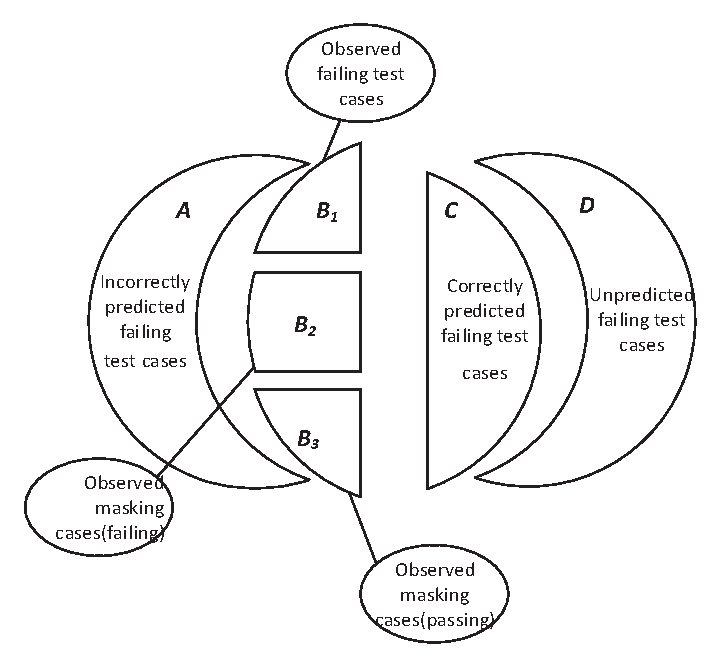
\includegraphics[width=3.51in]{FCI-mask.eps}
\caption{FCI with masking effects}
\label{fig:fci_mask}
\end{figure}

With this model, if we know which test cases mask the expected failure, i.e., if we have figured out $B_{2}$ and $B_{3}$, then the schemas that the FCI approach will identify can be described as $\mathcal{C}(A \bigcup B_{1} \bigcup B_{2} \bigcup C)$.  We next denote the condition that we have known the masking effects in prior as \emph{knowing masking effects}. However, as discussed before, to get this result is not possible without human involvement. Correspondingly, when using the \emph{regarded as one failure} strategy, the set of MFS traditional FCI identify is $\mathcal{C}(A \bigcup B_{1} \bigcup B_{2} \bigcup B_{3} \bigcup C)$.  And for the \emph{distinguishing failures} strategy, the MFS is $\mathcal{C}(A \bigcup B_{1} \bigcup C)$.

To be convenient, let  $T_{as} = B_{1} \bigcup B_{2} \bigcup C \bigcup D$ indicate all the actual failing test cases, $T_{km} = A \bigcup B_{1} \bigcup B_{2} \bigcup C$ indicate the test cases for strategy \emph{knowing masking effects}, $T_{ro} = A \bigcup B_{1} \bigcup B_{2} \bigcup B_{3} \bigcup C $ indicate the test cases for strategy \emph{regarded as one failure}, and $T_{df} = A \bigcup B_{1} \bigcup C$ indicate the test cases for strategy \emph{distinguishing failures}. Next, we will discuss the influence of masking effects on the two strategies.

\subsubsection{Using the regarded as one failure strategy}
For the strategy \emph{regarded as one failure}, the impacts of masking effects on FCI approaches can be analysed  by comparing the MFS identified by this strategy to those by strategy \emph{knowing masking effects}. Formally, it is to compare  $\mathcal{C}(T_{ro})$  with  $\mathcal{C}(T_{km})$.  Intuitively, $\mathcal{C}(T_{km})$ is more close to $\mathcal{C}(T_{as})$ than $\mathcal{C}(T_{ro})$. In other word, when using \emph{regarded as one failure} strategy,  the deviation between the identified MFS  and the actual MFS is larger than that of strategy \emph{knowing masking effects}.

The gap between the two strategies can be further analysed by studying the relationships between these two MFS set. As $T_{km} \subset T_{ro}$ , according to Proposition  \ref{pro:sls}, schemas in  $\mathcal{C}(T_{ro})$ can be identical to some schemas in $\mathcal{C}(T_{km})$, or be sub schemas of some of them, or irrelevant to all of them. Formally, $\forall c_{ro} \in \mathcal{C}(T_{ro}),\  \exists c_{km} \in \mathcal{C}(T_{km}),\ s.t.,\ c_{km} = c_{ro},\ or\ c_{ro} \prec c_{km},\ or\ c_{ro}\ irrelevant\ to\ \mathcal{C}(T_{km})$, three possibilities in total.

Now let us get back to the relationships between the schemas obtained by \emph{knowing masking effects} strategy and the actual MFS.  It can be found that test cases that are used for identifying the MFS using this strategy, i.e., $T_{km} $, \emph{intersect} the test cases that are used to compute the actual MFS( $ T_{as}$ ). According to Proposition \ref{pro:concludeforintersection}, the minimal schemas obtained by this strategy can be identical, super-schema, sub-schema, and irrelevant to the actual MFS, four possibilities in total. Formally, $\forall c_{km} \in \mathcal{C}(T_{km}),\ \exists c_{as} \in \mathcal{C}(T_{as}),\ s.t.,\ c_{as} = c_{km},\ or\ c_{km} \prec c_{as},\ or\ c_{as} \prec c_{km} \ or\ c_{km}\ irrelevant\ to\ \mathcal{C}(T_{as})$.

Take schema $c_{km}$ as intermediate schema, then for any schema $c_{ro}$ in $\mathcal{C}(T_{ro})$, the possible relationships between $c_{ro}$ and $c_{km}$, $c_{as}$ can be described in Table \ref{conditions-for-ro}. The same as Table \ref{possible-result-of-intersection}, one row can be described in the form of $\forall c_{ro} \in \mathcal{C}(T_{ro}),\ if\ \exists c_{km} \in \mathcal{C}(T_{km}),\ s.t.,\ ...$ and correspondingly, $\exists c_{as} \in \mathcal{C}(T_{as}),\ s.t,\ ...$, then it has $c_{ro} ... c_{as}$.  For example, the first scenario (ID 1) means that $\forall c_{ro} \in \mathcal{C}(T_{ro}),\ if\ \exists c_{km} \in \mathcal{C}(T_{km}),\ s.t.,\ c_{ro} = c_{km}$ and correspondingly, $\exists c_{as} \in \mathcal{C}(T_{as}),\ s.t,\ c_{km} = c_{as}$, then we have $c_{ro} = c_{as}$. The details of each row are described as propositions in Section A.1 in the Appendix. Some necessary proofs are also attached.

%We take $c_{km}$ as intermediate schema both has relationships between these two schemas as discussed before, second, we can clearly enure the difference between $c_{ro}$ and $c_{km}$, which can help to understand the impacts of masking effects for this strategy.

\begin{table}[h]
\centering
\tbl{Possible scenarios for Regard as one failure strategy \label{conditions-for-ro}}{
  \begin{tabular}{c|c|c||c} \hline
ID & $c_{ro}$ and $c_{km}$  &  $c_{km}$  and $c_{as}$  & $c_{ro}$  and $\mathcal{C}(T_{as})$ \\ \hline
%& & \\ \hline
1&$ c_{ro} = c_{km}  $    	&   $ c_{as} = c_{km}$    &    $c_{ro} = c_{as}$   \\
2&$  c_{ro} = c_{km}  $    	&   $ c_{as} \prec c_{km}$  &    $c_{as} \prec c_{ro}$      \\
3&$ c_{ro} = c_{km}  $    	&   $ c_{km} \prec c_{as}$  &    $c_{ro} \prec c_{as}$    \\
4&$ c_{ro} = c_{km}  $    	&   $c_{km}\ irrelevant \ \mathcal{C}(T_{as})$  &  $c_{ro}\ irrelevant\  \mathcal{C}(T_{as})$ \\
5&$ c_{ro} \prec c_{km} $    	&   $ c_{as} = c_{km}$   &   $c_{ro} \prec c_{as}$      \\
6&$ c_{ro} \prec c_{km} $    	&   $ c_{as} \prec c_{km}$  &  $\exists c_{as}', c_{ro} \prec c_{as}',\ or\ c_{ro}\ irrelevant\  \mathcal{C}(T_{as})$        \\
7&$ c_{ro} \prec c_{km} $    	&   $c_{km} \prec c_{as}$   &  $c_{ro} \prec c_{as}$     \\
8&$ c_{ro} \prec c_{km} $    	&   $c_{km}\ irrelevant  \ \mathcal{C}(as)$ & $\exists c_{as}, c_{ro} \prec c_{as},\ or\ c_{ro}\ irrelevant\  \mathcal{C}(T_{as})$  \\
9&$c_{ro}\ irrelevant \ to \ \mathcal{C}(T_{km}) $    	&   ---    & $\exists c_{as}, c_{ro} \prec c_{as},\ or\ c_{ro}\ irrelevant\  \mathcal{C}(T_{as})$      \\
 \hline \end{tabular}
  }
\end{table}

Table \ref{example-rule16} gives an example. In this table, Column `$A$', `$B_{3}$', `$D$' indicate the test cases of areas $A$, $B_{3}$, $D$, respectively, in Fig \ref{fig:fci_mask}. Column `$B_{1}\bigcup B_{2}\bigcup C$' indicates the union of test cases of areas $B_{1}$, $B_{2}$ and $C$. We did not distinguish them because this union is a common part of $\mathcal{C}(T_{as})$, $\mathcal{C}(T_{km})$ and $\mathcal{C}(T_{ro})$.  In the below part of this table, Column `$C(T_{as})$', `$C(T_{km})$' and `$C(T_{ro})$' show the actual MFS, schemas obtained by strategy \emph{knowing masking effects} and by \emph{regarded as one failure}, respectively.

\begin{table}[h]
\tbl{Example of relationships between three strategies \label{example-rule16}}{
\begin{tabular}{llllllllllll}
\multicolumn{3}{c}{\bfseries $A$} &\multicolumn{3}{c}{\bfseries $B_{1}\bigcup B_{2}\bigcup C$}  & \multicolumn{3}{c}{\bfseries $B_{3}$} & \multicolumn{3}{c}{\bfseries $D$}\\ \hline
\multicolumn{3}{c}{(1,1,1,0)}&\multicolumn{3}{c}{(1,1,0,0)}&\multicolumn{3}{c}{(1,0,0,1)}&\multicolumn{3}{c}{(0,1,0,0)}\\
\multicolumn{3}{c}{}&\multicolumn{3}{c}{(1,1,0,1)}&\multicolumn{3}{c}{(1,0,0,0)}&\multicolumn{3}{c}{(0,1,0,1)}\\

 \hline
\multicolumn{5}{c}{\bfseries $\mathcal{C}(T_{as})$} &\multicolumn{4}{c}{\bfseries $\mathcal{C}(T_{km})$} & \multicolumn{3}{c}{\bfseries $\mathcal{C}(T_{ro})$} \\ \hline
\multicolumn{5}{c}{(1,1,0,-)}             &\multicolumn{4}{c}{(1,1,0,-)} &           \multicolumn{3}{c}{(1,-,0,-)}\\
\multicolumn{5}{c}{(-,1,0,-)}             &\multicolumn{4}{c}{(1,1,-,0)} &           \multicolumn{3}{c}{(1,1,-,0)}\\
%\multicolumn{4}{c}{}             &\multicolumn{4}{c}{} &           \multicolumn{4}{c}{}\\
  \hline

%\multicolumn{4}{c}{\bfseries rules} &\multicolumn{2}{c}{\bfseries $c_{m}$}  & \multicolumn{2}{c}{\bfseries $c_{origin}$} & \multicolumn{2}{c}{\bfseries $c_{new}$} & \multicolumn{2}{c}{\bfseries $c_{m}'$}\\ \hline
%\multicolumn{4}{c}{ 2} &\multicolumn{2}{c}{(1,-,1,1,-,0)}  & \multicolumn{2}{c}{(1,-,1,1,-,0)} & \multicolumn{2}{c}{(1,-,1,-,-,0)} & \multicolumn{2}{c}{(1,-,1,1,-,0)}\\

\end{tabular}
}
\end{table}

Let $c_{ro}$ = (1,-,0,-), then we have $c_{km} $ = (1,1,0,-) so that $c_{ro} \prec c_{km}$. Further, it is found that $c_{as}$ = (1,1,1,0), which is equal to $c_{km}$. At last we have $c_{ro} \prec c_{as}$. This corresponds scenario 5 in Table \ref{conditions-for-ro}. Additionally, if let $c_{ro}$ = (1,1,-,0), and obviously $c_{km}$ = (1,1,-,0) is equal to $c_{ro}$. Then we can find that $c_{km}$ is irrelevant to all the schemas in  $\mathcal{C}(T_{as})$, and so is $c_{ro}$. This corresponds scenario 4 in Table \ref{conditions-for-ro}.  We do not include all the scenarios in this example,  but others (scenarios 1,2,3,6,7,8) can be easily constructed in a similar way.

From Table \ref{conditions-for-ro}, it can be found that for any schema identified by strategy \emph{regarded as one failure}, it can be identical to the actual MFS (scenario 1), or be subschema (scenarios 3, 5, 7, 8, 9), or super schema (scenario 2), or irrelevant to all the actual MFS (scenarios 4, 6,8,9). Among those possibilities, the schemas obtained by strategy \emph{regarded as one failure} are more likely to be subschemas and irrelevant ones when comparing with strategy \emph{knowing masking effects}.

Apart from these four possible relationships between schema $c_{ro}$ and $\mathcal{C}(T_{as})$, it is also desired to learn the extent to which the actual MFS is irrelevant to the schemas identified by strategy \emph{regarded as one failure}, i.e., to learn how much the actual MFS is \emph{ignored}. To figure this out, we need to take schema $c_{as}$ as the subject, and then find the relationships  between it and schemas $c_{km}$, $c_{ro}$. Similar as Table \ref{conditions-for-ro}, we take schema $c_{km}$ as intermediate schema. Then for any schema $c_{as}$, the possible relationships between it and the other two kinds schemas can be described in Table \ref{conditions-for-ro-ignore}. The same as before, we list the detail explanation of each row in section A.2 in the Appendix. It is noted that scenarios 4 and 7 (marked star) in Table \ref{conditions-for-ro-ignore} will make the corresponding actual MFS ignored, which indicates that strategy \emph{regarded as one failure} is a bit higher than \emph{knowing masking effects} at ignoring the actual MFS.

\begin{table}[h]
\centering
\tbl{Possible conditions for Regard as one failure strategy --ignoring \label{conditions-for-ro-ignore}}{
  \begin{tabular}{c|c|c||c} \hline
ID & $c_{as}$ and $c_{km}$  &  $c_{km}$  and $c_{ro}$  & $c_{as}$  and $\mathcal{C}(T_{ro})$ \\ \hline
%& & \\ \hline
1&  $ c_{as} = c_{km}$   	    &   $ c_{ro} = c_{km}  $    &     $c_{ro} = c_{as}$   \\
2&  $ c_{as} = c_{km}  $       	&   $ c_{ro} \prec c_{km}$  &     $c_{ro} \prec c_{as}$      \\
3&  $ c_{as} \prec c_{km}  $    &   $ c_{ro} = c_{km}$      &     $c_{as} \prec c_{ro}$    \\
4$\star$&  $ c_{as} \prec c_{km}  $    &   $ c_{ro} \prec c_{km} $ &     $c_{as}\ irrelevant\  \mathcal{C}(T_{ro})$ or $c_{as} \prec c_{ro}'$ \\
5&  $ c_{km} \prec c_{as} $    	&   $ c_{ro} = c_{km}$      &     $c_{ro} \prec c_{as}$      \\
6&  $ c_{km} \prec c_{as} $    	&   $ c_{ro} \prec c_{km}$  &     $c_{ro} \prec c_{as}$        \\
7$\star$ &  $ c_{as}\ irrelevant \ to \ \mathcal{C}(T_{km})$    	&   ---   &  $ c_{as}\ irrelevant\ \mathcal{C}(T_{ro})$   \\
 \hline \end{tabular}
  }
\end{table}

An example of the ignoring scenario is also in Table \ref{example-rule16}. Let $c_{as}$ = (-,1,0,-), it is irrelevant to all the schemas in  $\mathcal{C}(T_{km})$. As it is also irrelevant to $\mathcal{C}(T_{ro})$, so it corresponds scenario 7 in Table \ref{conditions-for-ro-ignore}. Other scenarios can also be easily constructed, which will not be omitted in this paper.

\subsubsection{Using distinguishing strategy}
%Another point need to be noted is that this also mean some ignored ones(As MFS irrelevant to the set). That with this strategy, will get more ignored ones.
For this strategy, the set of test cases that are used to compute the minimal schemas is subset of that of strategy \emph{knowing masking effects}, i.e., $T_{df} \subset T_{km}$. According to Proposition  \ref{pro:ssp}, schemas in  $\mathcal{C}(T_{ro})$ can be identical to some schemas in $\mathcal{C}(T_{km})$, or be super schemas of some of them. Formally, $\forall c_{df} \in \mathcal{C}(T_{df}),\  \exists c_{km} \in \mathcal{C}(T_{km}),\ s.t.,\ c_{km} = c_{ro},\ or\ c_{km} \prec c_{df}$, two possibilities in total. Combining the relationships between the schemas obtained by \emph{knowing masking effects} strategy and the actual MFS, then for any schema $c_{df}$ in $\mathcal{C}(T_{df})$, there are 8 possible scenarios between $c_{df}$ and other two kinds of schemas ($c_{km}, c_{as}$), which are shown as in Table \ref{conditions-for-df}. Similar as Table \ref{conditions-for-ro}, the detail explanation of each row is shown in Section A.3 in the Appendix.


\begin{table}[h]
\centering
\tbl{Possible conditions for Distinguishing failures strategy \label{conditions-for-df}}{
  \begin{tabular}{c|c|c||c} \hline
ID & $c_{df}$ and $c_{km}$  &  $c_{km}$  and $c_{as}$  & $c_{df}$  and $\mathcal{C}(T_{as})$ \\ \hline
%& & \\ \hline
1&$ c_{df} = c_{km}  $    	&   $ c_{as} = c_{km}$    &    $c_{df} = c_{as}$   \\
2&$  c_{df} = c_{km}  $    	&   $ c_{as} \prec c_{km}$  &    $c_{as} \prec c_{df}$      \\
3&$ c_{df} = c_{km}  $    	&   $ c_{km} \prec c_{as}$  &    $c_{df} \prec c_{as}$    \\
4&$ c_{df} = c_{km}  $    	&   $c_{km}\ irrelevant \ \mathcal{C}(T_{as})$  &  $c_{df}\ irrelevant\  \mathcal{C}(T_{as})$ \\
5&$ c_{km} \prec c_{df} $    	&   $ c_{as} = c_{km}$   &   $c_{as} \prec c_{df}$      \\
6&$ c_{km} \prec c_{df} $    	&   $ c_{as} \prec c_{km}$  &  $c_{as} \prec c_{df}$        \\
7&$ c_{km} \prec c_{df} $    	&   $c_{km} \prec c_{as}$   &  $\exists c_{as}',\ s.t.,\ c_{df} = c_{as}',\ or\ c_{as}' \prec c_{df}$     \\
 &                           	&                           &  $ \ or\ c_{df} \prec c_{as}',\ or\ c_{df}\ irrelevant\  \mathcal{C}(T_{as})$     \\
8&$ c_{km} \prec c_{df} $    	&   $c_{km}\ irrelevant  \ \mathcal{C}(as)$ & $\exists c_{as}, c_{as} \prec c_{df} ,\ or\ c_{df}\ irrelevant\  \mathcal{C}(T_{as})$  \\

%9&  $c_{km}\ irrelevant \ to \ \mathcal{C}(T_{df})$    	&   --- & \textbf{may} $c_{as}\ irrelevant\  \mathcal{C}(T_{df})$    \\
%
%10&   --- 	&   $c_{as}\ irrelevant\ to\ \mathcal{C}(T_{km})$     &   $c_{as}\ irrelevant\  \mathcal{C}(T_{df})$  \\  \hline

%10a&  $c_{km}\ irrelevant \ to \ \mathcal{C}(T_{df})$    	&   $ c_{as} = c_{km}$  &  ---     \\
%10b&  $c_{km}\ irrelevant \ to \ \mathcal{C}(T_{df})$    	& $ c_{as} \prec c_{km}$    & ---     \\
%10c&  $c_{km}\ irrelevant \ to \ \mathcal{C}(T_{df})$    	& $ c_{km} \prec c_{as}$   & ---     \\
%10d&  $c_{km}\ irrelevant \ to \ \mathcal{C}(T_{df})$    	&   $c_{km}\ irrelevant \ \mathcal{C}(T_{as})$ & ---    \\
 \hline \end{tabular}
  }
\end{table}

One observation of this table is that when comparing with strategy \emph{knowing masking effects}, the schemas identified by strategy \emph{distinguishing failures} are more likely to be super schemas of the actual MFS (scenarios 2, 5,6,7,8) and irrelevant ones (scenarios 4,7,8).  Comparing with strategy \emph{regarded as one failure}, however, the schemas that identified by this strategy are less likely to be irrelevant to all the actual MFS. This is because strategy \emph{regarded as one failure} has four scenarios (scenarios  4, 6,8,9 in Table \ref{conditions-for-ro}) which can make the schemas to be irrelevant ones.

Table \ref{example-rule26} gives an example of this strategy. In this table, Column `$A$', `$B_{2}$', `$D$' indicate the test cases of areas $A$, $B_{2}$, $D$, respectively, in Fig \ref{fig:fci_mask}. Column `$B_{1} \bigcup C$' indicates the union of test cases of areas $B_{1}$, and $C$, which is a common part of $\mathcal{C}(T_{as})$, $\mathcal{C}(T_{km})$ and $\mathcal{C}(T_{df})$.  In the below part of this table, Column `$C(T_{as})$', `$C(T_{km})$' and `$C(T_{df})$' show the actual MFS, schemas obtained by strategy \emph{knowing masking effects} and by \emph{distinguishing failures}, respectively.

\begin{table}[h]
\tbl{Example of rule 6 in Table \ref{conditions-for-df} \label{example-rule26}}{
\begin{tabular}{llllllllllll}
%\multicolumn{3}{c}{} &\multicolumn{3}{c}{}  & \multicolumn{3}{c}{} & \multicolumn{3}{c}{}\\
\multicolumn{3}{c}{\bfseries $A$} &\multicolumn{3}{c}{\bfseries $B_{1}\bigcup C$}  & \multicolumn{3}{c}{\bfseries $B_{2}$} & \multicolumn{3}{c}{\bfseries $D$}\\ \hline

\multicolumn{3}{c}{(1,1,1,0)}&\multicolumn{3}{c}{(1,1,0,0)}&\multicolumn{3}{c}{(1,0,0,1)}&\multicolumn{3}{c}{(0,1,0,0)}\\
\multicolumn{3}{c}{}&\multicolumn{3}{c}{(1,1,0,1)}&\multicolumn{3}{c}{(1,0,0,0)}&\multicolumn{3}{c}{(0,1,0,1)}\\
 \hline

\multicolumn{5}{c}{\bfseries $\mathcal{C}(T_{as})$} &\multicolumn{4}{c}{\bfseries $\mathcal{C}(T_{km})$} & \multicolumn{3}{c}{\bfseries $\mathcal{C}(T_{df})$} \\ \hline
\multicolumn{5}{c}{(1,-,0,-)}             &\multicolumn{4}{c}{(1,-,0,-)} &           \multicolumn{3}{c}{(1,1,0,-)}\\
\multicolumn{5}{c}{(-,1,0,-)}             &\multicolumn{4}{c}{(1,1,-,0)} &           \multicolumn{3}{c}{(1,1,-,0)}\\

%\multicolumn{4}{c}{\bfseries $\mathcal{C}(B_{1} \bigcup B_{2} \bigcup C \bigcup D )$} &\multicolumn{4}{c}{\bfseries $\mathcal{C}(A \bigcup B_{1} \bigcup B_{2} \bigcup C)$} & \multicolumn{4}{c}{\bfseries $\mathcal{C}(A \bigcup B_{1} \bigcup C)$} \\ \hline

\hline \end{tabular}}
\end{table}

Let $c_{df}$ = (1,1,0,-), then we have $c_{km} $ = (1,-,0,-) so that $c_{km} \prec c_{df}$. Further, it is found that $c_{as}$ = (1,-,1,-), which is equal to $c_{km}$, so $c_{as} \prec c_{df}$. This corresponds scenario 5 in Table \ref{conditions-for-df}.  If let $c_{df}$ = (1,1,-,0), and obviously $c_{km}$ = (1,1,-,0) is equal to $c_{df}$. As  $c_{km}$ is irrelevant to all the schemas in  $\mathcal{C}(T_{as})$, then $c_{ro}$ is also irrelevant to $\mathcal{C}(T_{as})$. This corresponds scenario 4 in Table \ref{conditions-for-df}. The same as Section 4.2.1, other scenarios are omitted in this example, which can be constructed in a similar way.

Next, the ingoring state, i

\begin{table}[h]
\centering
\tbl{Possible conditions for Distinguishing failures strategy --ignoring \label{conditions-for-df-ignore}}{
  \begin{tabular}{c|c|c||c} \hline
ID & $c_{as}$ and $c_{km}$  &  $c_{km}$  and $c_{df}$  & $c_{as}$  and $\mathcal{C}(T_{df})$ \\ \hline
%& & \\ \hline
1&  $ c_{as} = c_{km}$   	    &   $ c_{df} = c_{km}  $    &     $c_{df} = c_{as}$   \\
2&  $ c_{as} = c_{km}  $       	&   $ c_{km} \prec c_{df}$  &     $c_{as} \prec c_{df}$      \\
3$\star$&  $ c_{as} = c_{km}  $       	&   $ c_{km}\ irrelevant\ \mathcal{C}(T_{df})$  &  $ c_{as}\ irrelevant\ \mathcal{C}(T_{df})$        \\
4&  $ c_{as} \prec c_{km}  $    &   $ c_{df} = c_{km}$      &     $c_{as} \prec c_{df}$    \\
5&  $ c_{as} \prec c_{km}  $    &   $ c_{km} \prec c_{df} $ &     $c_{as} \prec c_{df}$ \\
6$\star$&  $ c_{as} \prec c_{km}  $    &   $ c_{km}\ irrelevant\ \mathcal{C}(T_{df})$ &     $c_{as}\ irrelevant\  \mathcal{C}(T_{df})$ or $c_{df} \prec c_{as}$ \\
7&  $ c_{km} \prec c_{as} $    	&   $ c_{df} = c_{km}$      &     $c_{df} \prec c_{as}$      \\
8$\star$&  $ c_{km} \prec c_{as} $    	&   $ c_{km} \prec c_{df}$  &     $c_{as}\ irrelevant\  \mathcal{C}(T_{df})$ or $c_{df}' \prec c_{as}$        \\
 &                            	&                           &    or $\ c_{as} \prec c_{df}' $ or $c_{df}'  =  c_{as}$        \\
9$\star$&  $ c_{km} \prec c_{as} $    	&   $ c_{km} irrelevant\ \mathcal{C}(T_{df})$ &     $c_{as}\ irrelevant\  \mathcal{C}(T_{df})$ or $c_{df} \prec c_{as}$     \\
10$\star$&  $ c_{as}\ irrelevant \ to \ \mathcal{C}(T_{km})$    	&   ---   &  $ c_{as}\ irrelevant\ \mathcal{C}(T_{ro})$   \\
%8&  $ c_{ro} \prec c_{km} $    	&   $c_{km}\ irrelevant  \ \mathcal{C}(as)$ & $\exists c_{as}, c_{ro} \prec c_{as},\ or\ c_{ro}\ irrelevant\  \mathcal{C}(T_{as})$  \\
%9&  $c_{ro}\ irrelevant \ to \ \mathcal{C}(T_{km}) $    	&   ---    & $\exists c_{as}, c_{ro} \prec c_{as},\ or\ c_{ro}\ irrelevant\  \mathcal{C}(T_{as})$      \\
%10&  ---  	&   $c_{as}\ irrelevant\ to\ \mathcal{C}(T_{km})$     &   $c_{as}\ irrelevant\  \mathcal{C}(T_{ro})$  \\
 \hline \end{tabular}
  }
\end{table}


\subsection{Summary of the masking effects on the FCI approach}
From the analysis of the formal model, we can learn that masking effect does influence the FCI approaches, and even worse, both the \emph{regarded as one failure} and \emph{distinguishing failures} strategies have their own problems in handling this effect. Specifically when compared with the \emph{knowing masking effects} condition, the strategy \emph{regarded as one failure} has a larger possibility of getting more sub-schemas of the actual MFS and getting more schemas which are irrelevant to the MFS, while strategy \emph{distinguishing failures}  may get more super schemas of the MFS and can also get more irrelevant MFS. Further, both strategies may ignore the actual MFS with the \emph{distinguishing failures} strategy more likely to ignore the MFS than the \emph{regarded as one failure} strategy.

%Note that our discussion is based on a SUT using deterministic software, i.e., the random failing information of a test case will be ignored. The non-deterministic problem will result in a more complex test scenario, which will not be discussed in this paper.

\section{Test case replacing strategy}
%Previous section formally studied the case that under the masking effects, neither regarding as one failure approach nor distinguishing failures approach is not accurate .
The main reason that the FCI approach fails to work properly is that it cannot determine $B_{2}$ and $B_{3}$, i.e., if the test case triggers other failures which are different from the currently analysed one, it cannot figure out whether this test case will trigger the current expected failure because of the masking effects. So to limit the impact of this effect on the FCI approach, it is important to reduce the number of test cases that trigger other different failures, as it can reduce the probability that expected failure may be masked by other failures.
% strategies cannot accurately identify the MFS is that we cannot figure out the $T(mask_{F_{m}})$.  As $T(mask_{F_{m}}) \subset \bigcup_{i = 1 \& i \neq m }^{L}T_{F_{i}}$, in order to weaken the influence of $T(mask_{F_{m}})$, we need to reduce the number of test cases that trigger other failures as much as possible.

In the exhaustive testing, as all the test cases will be used to identify the MFS, there is no room left to improve the performance unless we fix other failures and re-execute all the test cases. However, if only a subset of all test cases is used to identify the MFS (which is how the traditional FCI approach works), it is important to make the right selection to limit the size of $\mathcal{T}(mask_{F_{m}})$ to be as small as possible.

\subsection{Replacing test cases that trigger unexpected failures}

The basic idea is to pick the test cases that trigger other failures and generate new test cases to replace them. The regenerated test cases should either pass in the execution or trigger $F_{m}$. The replacement must satisfy the condition that the newly generated ones will not negatively influence the original identifying process.

Normally, when we replace the test case that triggers an unexpected failure with a new test case, we should keep some part of the original test case. We call this part the \emph{fixed part}, and mutate the other part with different values from the original one. For example, if a test case (1,1,1,1) triggered an unexpected failure, and the fixed part is (-,-,1,1). Then, we can replace it with a test case (0,0,1,1) which may either pass or trigger the expected failure.

The \emph{fixed part} can vary for different FCI approaches, e.g, for the OFOT \cite{nie2011minimal} algorithm, the parameter values are the fixed part except for the one that needs to be validated, while for the FIC\_BS \cite{zhang2011characterizing} approach, the fixed parts are dynamically changed, depending on the outcome of the execution of last generated test case.

This replacement may need to be executed multiple times for one fixed part as it may not always possible to find a test case that coincidentally satisfied our requirement. One replacement method is randomly choosing test cases until the satisfied test case is found. While this method may be simple and straightforward, however, it also may require trying many times. So to handle this problem and reduce the cost, we propose a replacement approach by computing the \emph{strength} of the test case with the other failures, and then we select the test case from a group of candidate test cases that has the least \emph{strength} related to the other failures.

% which during the originally test, record the test cases that trigger other test cases and next replacement process will consult this set to avoid some test cases with a high probability to trigger other failures.

To explain the \emph{strength} notion, we first introduce the \emph{strength} that a parameter value is related to a particular failure. We use $all(o)$ to represent the number of executed test cases that contain this parameter value, and $m(o)$ to indicate the number of test cases that trigger the failure $F_{m}$ and contain this parameter value. Then, the \emph{strength} that a parameter value is related to a particular failure, i.e., $S(o, F_{m})$, is $\frac{m(o)}{all(o) + 1}$. This heuristic formula is based on the idea that if a parameter value frequently appears in the test cases that trigger a particular failure, then it is more likely to be the inducing factor that triggers this failure. We add 1 in the denominator for two reasons:  (1) avoid division by zero when the parameter value has never appeared before, (2) reduce the bias when a parameter value rarely appears in the test set but coincidentally appears in a failing test case with a particular failure.

With the \emph{strength} associated with a parameter value, we then define the \emph{strength} of a test case $f$ is related to a particular failure $F_{m}$ as:

\begin{displaymath} S(f,F_{m})  = \frac{1}{k}\sum_{o \in f} S(o, F_{m}) \tag{EQ1} \label{eqn - 00p} \end{displaymath}

where $k$ is the number of parameters in $f$, and $o$ is the specific parameter value in $f$. The \emph{strength} that a test case is related to a failure is defined as the average \emph{strength} of the relevance between each parameter value in the test case and this failure. For a selected test case, we want its ability  to trigger another failure to be as small as possible, such that the masking effects can be alleviated. In practice, the relevance \emph{strength} varies between test case with different failures. As a result, we cannot always find a test case that, for any failure, the \emph{strength} that this test case is related to that failure is the least.  With this in mind, we have to settle for a test case, such that the maximal possible failure (except for the one that is currently analysed) it can trigger should be the least likely to be triggered when compared with that of other test cases. In other word, we need to find a test case, so that the maximal \emph{strength} that it is related to another failure is minimal. Formally, we should choose a test case $f$, s.t.,

\begin{displaymath} \min_{f \in R} \max_{m \leq L \& m \neq n}  S(f, F_{m}) \tag{EQ2} \label{eqn - 0p}\end{displaymath}

where $L$ is the number of failures, and $n$ is the current analysed failure. $R$ is the set of all possible test cases that contain the $fixed$ part except those that have been tested. The test case is from the set $R$ because the FCI approach needs to keep the $fixed$ part when generating additional test cases and the test case should not have been executed. Obviously $|R| = \prod_{i \not\in fixed}(v_{i})\ - |\{t\ |\ t\ contains\ the\ fixed\ part\ \&\ t\ is\ executed\}|$.

We can further resolve this problem. Consider the test case $f$ satisfies \ref{eqn - 0p}. Without loss of generality, we assume that the failure $F_{k}, k \neq n $ is the failure with which the test case $f$ has the maximal related \emph{strength} compared to the other failures. Then, a natural property for $f$ is that any other test case $f'$ which satisfies that failure $F_{k}$ is the maximal related failure for this test case
and must have $ S(f, F_{k}) <= S(f', F_{k})$. Formally, to obtain such a test case is to solve the following formula:

\begin{alignat}{2}
\min\quad &  S(f, F_{k}) &{}& \tag{EQ3} \label{eqn - lp}\\
\mbox{s.t.}\quad
&f \in R &\quad& {}\nonumber\\
&S(f, F_{k}) > S(f, F_{i}), &{}& 1 \leq i \leq L\ \&\ i\neq k, n \nonumber
\end{alignat}

To solve \ref{eqn - 0p}, we just need to find a particular failure $F_{k}$, and the corresponding test case $f_{k}$ that satisfies \ref{eqn - lp}, such that the related \emph{strength} between  $f_{k}$ and $F_{k}$ is smaller than the related \emph{strength} between any other failures and their corresponding test cases that satisfy \ref{eqn - lp}. Formally, we need to find:
\begin{alignat}{2}
\min\quad &  S(f, F_{k}) &{}& \tag{EQ4} \label{eqn - 2p}\\
\mbox{s.t.}\quad
& 1 \leq k \leq L \ \& \ k \neq n &\quad& {}\nonumber\\
& f , F_{k}\ satisfies\ \ref{eqn - lp} &{}& {} \nonumber
\end{alignat}

According to \ref{eqn - 2p}, to determine such a test case lies in solving \ref{eqn - lp} because if it is solved we just need to rank the one that has the minimal value from the solutions to \ref{eqn - lp}. As to \ref{eqn - lp}, it can be formulated as an 0-1 integer linear programming (ILP) problem. Assume the SUT has $K$ parameters in which the $i$th parameter has $V_{i}$ values. And the SUT has $L$ failures. We then define the variable $x_{ij}$ as:
\begin{displaymath}
x_{ij} = \begin{cases}1 & the\ \emph{i}th\ parameter\ of\ the\ test\ case\ take\ the\ \emph{j}th\ value\ for\ that\ parameter\\0 & otherwise\end{cases}
\end{displaymath}
We then take $o_{m_{ij}}$ to be the related \emph{strength} between the \emph{j}th value of the \emph{i}th parameter of the SUT and the failure $F_{m}$. And we use a set $R$ of parameter values to define the fixed part in the test case we should not change, i.e., $R = \{(i, j) |i\ is\ the\ fixed\ parameter\ in\ the\ test\ case, j\ is\ the\ corresponding\ value\}$. As we can generate redundant test cases, so we keep a set of test cases $T_{executed}$ to guide the generation of different test cases. Then \ref{eqn - lp} can be transformed into following ILP formula:

\begin{alignat}{2}
\min\quad & \frac{1}{|K|}\sum_{i = 0}^{K}\sum_{j = 0}^{V_{i}}  o_{m_{ij}} \times x_{ij} &{}& \tag{EQ5} \label{eqn - 3p}\\
\mbox{s.t.}\quad
& 0 \leq x_{ij} \leq 1 &\quad& { i = 0 .. K - 1, j = 0,.. V_{i} - 1 }\\
&  x_{ij} \in  \mathbb{Z}&\quad& { i = 0 .. K - 1, j = 0,.. V_{i} - 1 }\\
& \sum_{j = 0}^{V_{j}} x_{ij} = 1&\quad& { i = 0 ... K - 1}\\
&  x_{ij} = 1 &\quad& { (i,j) \in R }\\
& \sum_{i = 0}^{K}\sum_{j = 0}^{V_{i}} (o_{m_{ij}} - o_{m'_{ij}})\times  x_{ij} \geq 0 &\quad& {1 \leq m' \neq m \leq L}\\
& \sum_{(i,j) \in t}  x_{ij} < K &\quad& {t \in T_{existed}}
\end{alignat}

In \ref{eqn - 3p}, constraints (1) and (2) indicate that the variable $x_{ij}$ is a 0-1 integer. Constraint (3) indicates that a parameter in one test case can only take on one value. Constraint (4) indicates that the test case should not change values of the fixed part. Constraint (5) indicates that the related strength between the test case and failure $F_{m}$ is higher than that of the other failures. Constraint (6) indicates that the test cases generated should not be the same as the test cases in $T_{existed}$.

As we have formulated the problem into a 0-1 integer programming problem, we just need to utilize an ILP solver to solve this formula. In this paper, we use the solver introduced in \cite{Berkelaar2004}, which is a mixed Integer Linear Programming (MILP) solver that can handle satisfaction and optimization problems.
%this actually an integer programming problem, as the test case $f$ is the vector of component $o$, which is concrete variable. However, it dose not belongs to the integer linear programming (ILP) problem, because the objective function  $S(f, F_{k})$, i.e., $\frac{1}{|f|}\sum_{o \in f} S(o, F_{m})$, is not linear to the component $o$.
%s.t.
%
%S(f, F_{k}) > S(f, F_{1})
%S(f, F_{k}) > S(f, F_{2})
%...
%S(f, F_{k}) > S(f, F_{n-1})
%S(f, F_{k}) > S(f, F_{n+1})
%...
%S(f, F_{k}) > S(f, F_{L})
% So to make it as less as possible is actually make the test case $f$ less related to other failures.



\begin{algorithm}[t]
%\SetAlgoNoLine
\KwIn{ failure $F_{m}$,fixed part $s_{fixed}$, set of values that each option can take $Param$, the related strength matrix $o_{1} ... o_{L}$}
\KwOut{ $t_{new}$ the regenerate test case,The frequency number }
%$index$ = 0; $FreNum_{\alpha}$ = -1\;
\While{\textbf{not} MeetEndCriteria()}{
       $optimal \leftarrow MAX$ ;
       $t_{new} \leftarrow null$ \;
       \ForAll {$F_{k} \in {F_{1},...F_{m}, F_{m+1} ... F_{L}}$}{
                $solver \leftarrow setup(s_{fixed}, Param, F_{m}, o_{1} ... o_{L})$\;
                $(optimal', t_{new}') \leftarrow solver.getOptimalTest()$ \;
                \If {$optimal' < optimal$}{
                       $t_{new} \leftarrow t_{new}'$\;
                    }
          }
       $result \leftarrow execute(t_{new})$\;
       $updatetRelatedStrengthMatrix(t_{new})$ \;
        \eIf {$result == PASS\ or\ result ==  F_{m}$}{
         \Return $t_{new}$\;
           }{
         continue\;
         }
       }
       \Return \emph{null}

\caption{Replacing test cases triggering unexpected failures}
\label{alg:one}
\end{algorithm}
The complete process of replacing a test case with a new one while keeping some fixed part is depicted in Algorithm 1.

The inputs to this algorithm consist of the failure $F_{m}$, the fixed part of which we want to keep from the original test case $s_{fixed}$ , the set of values that each parameter can take $Param$ and the set of matrix $o_{1},o_{2},...o_{m},...,o_{L}$, where $o_{m}$ ( $1 \leq m \leq L $ ) is recorded the related strength between each specific parameter with each value and the failure $F_{m}$, i.e., $o_{m} = \{o_{m_{ij}} | 0 \leq i \leq K - 1, 0 \leq j \leq V_{i}\}$. The output of this algorithm is a test case $t_{new}$ which either triggers the expected $F_{m}$ or passes.

The outer loop of this algorithm (lines 1 - 19) contains two parts:

The first part (lines 2 - 9) generates a new test case which is supposed to be least likely to trigger failures different from $F_{m}$. The basic idea for this part is to search each failure different from $F_{m}$ (line 3) and find the best test case that has the least related strength with other failures. In detail, for each failure we set up an ILP solver (line 4) and use it to get an optimal test case for that failure according to \ref{eqn - 3p} (line 5). We compare the optimal value for each failure, and choose the one with less strength related to other failures (lines 6 - 9).
%Different from the original algorithm, we generate a set of candidate test cases (line 3 - 11) instead of only one, and then choose the one that has the least possibility that is related to other failures(line 12) according to our previous formula. Our candidate set of test cases is initialed as size \emph{N}, the specific number it is assigned is a tradeoff between how quickly this algorithm ended in getting a candidate test case and how many times you'd like to try to find a really satisfied test case. It is noted that when \emph{N} = 1, it grows into our previous algorithm. Each test cases in the candidate set is generated by random(line 4 - 11), they must be different from existed test cases(we don't show in this pseudo code) and each one of them should keep the fixed part (line 9), and just mutate the factors which are not in that part(line 2). The mutation for each factor works by selecting one legal value which is different from the original one(line 5 - 8).
%The generated newly test case must be different from each iteration(we implemented it by hashing method).

The second part is to check whether the newly generated test case is as expected (lines 10 - 16). We first execute the SUT under the newly generated test case (line 10) and update the related strength matrix ($o_{1} ... o_{L}$) for each parameter value that is involved in this newly generated test case (line 11). We then check the execution result. If the test case passes or triggers the same failure -- $F_{m}$, a satisfied test case is obtained (line 12) and returned (line 13). Otherwise, we will repeat the process, i.e., generate a new test case and check again (lines 14 - 15).

Note that this algorithm has another exit, besides finding an expected test case (line 12), which is when the function \emph{MeetEndCriteria()} returns \emph{true} (line 1). We did not explicitly show function \emph{MeetEndCriteria()}, because this is dependent on the computing resource and the desired accuracy. In detail, if we want to get a high quality result and have enough computing resource, it is desirable to try many times to get the expected test case; otherwise, a relatively small number of attempts is recommended.

In this paper, we just set 3 as the greatest number of iterations for this function. When it ends with \emph{MeetEndCriteria()} returning true, it will return null (line 18), which means we cannot find an expected test case.

\subsection{A case study using the replacement strategy}
%Next we will take the FCI approach--OFOT algorithm as the subject to see how our approach works on them.

Suppose we have to test a system with eight parameters, each of which has three options. And when we execute the test case $T_{0}$ -- (0, 0, 0, 0, 0, 0, 0, 0), a failure--$e1$ is triggered. Furthermore, there are two more potential failures, $e2$ and $e3$, that may be triggered during the testing; and they will mask the desired failure $e1$. Next, we will use FIC\_BS \cite{zhang2011characterizing} with replacement strategy to identify the MFS for $e1$.  The process is shown in Figure \ref{fig:fci_case_study}. In this figure, there are two main columns. The left main column indicates the executed test cases during testing as well as the executed results, and each executed test case corresponds to a specific label, $T_{1}$ -- $T_{8}$, at the left. The right main column lists the related strength matrix when a test case triggers $e2$ or $e3$. In detail, the matrix records the related strength between each parameter (Columns $P1$ -- $P8$) for each value it can take (Column v) with the unexpected failure (Column F). The executed test case, shown in bold, indicates the one that triggers the other failure and should be replaced in the next iteration.
%the test case which are labeled with a deleted line represent the original test case generated by OFOT, and it will be replaced by the regenerated test case which are labeled with a wave line under it.

The completed MFS identifying process listed in Figure \ref{fig:fci_case_study} works as follows: firstly the original FCI approach determines which $fixed$ part needed to be test in each iteration. Then the extra test case will be generated to fill in the remaining part. After executing the extra test case, if the result of the execution is normal, i.e., did not trigger unexpected failure ($e_{2}, e_{3}$), then the original FCI process will continue until the MFS is identified. Otherwise,  the replacement strategy starts when an unexpected failure is triggered. The replacement process will mutate the parameter values that is not in the $fixed$ part according to Algorithm 1. After the replacement process, the control for the MFS identifying process will be passed back to the original FCI approach.  Next we will specifically explain how the replacement works with an example in this figure.

From Figure \ref{fig:fci_case_study}, for the test case that triggered $e2$ -- (2, 1, 1, 1, 0, 0, 0, 0) (in this case, the fixed part of the test case is (-, -, -, -, 0, 0, 0, 0), in which the last four parameter values are the same as the original test case $T_{0}$), we generate the related matrix at left. Each element in this matrix is computed as $\frac{m(o)}{all(o) + 1}$; for example, for the $P7$ parameter with value $0$, we can find two test cases that contain this element, i.e., $T_{0}$ and $T_{1}$, so $all(o)$ is 2. And only one test case triggers the failure $e2$, which means m(o) = 1. So the final related strength between this parameter value with $e2$ is $\frac{1}{2 + 1} = 0.33$. All the related strength with $e3$ is labeled with a short slash as there is no test case triggering this failure in this iteration.  After this matrix has been determined, we can obtain the optimal test case with the ILP solver, which is $T_{1}'$--(1, 2, 2, 2, 0, 0, 0, 0), with its related strength 0.167, which is smaller than that all.

This replacement process is started each time a new test case that triggered another failure until we finally get the MFS. Sometimes we could not find a satisfied replacing test case in just one trial like $T_{1}$ to $T_{1}'$.  When this happened, we needed to repeat searching the proper test case. For example, for $T_{4}$ which triggered $e3$, we tried three times-- $T_{4}', T_{4}'', T_{4}'''$ to finally get a satisfied $T_{4}'''$ which passes the testing. Note that the \emph{related strength} matrix continues to change as the test case is generated and executed so that we can adaptively find an optimal one.
% as in this iteration we did not find the test case triggered .
%
%randomly generate three test cases as the candidate test cases, which are (2 1 0 0 0 0 0 0), (2 2 0 0 0 0 0 0), (1 2 0 0 0 0 0 0) respectively.  For one candidate test case in the set--(2 1 0 0 0 0 0 0), the \emph{strength} it is related to the $Err 2$ can be computed as
%
%$$\frac{1}{8} (\frac{0}{1 + 1} + \frac{1}{1 + 1} + \frac{1}{2 + 1}  + \frac{1}{2 + 1} + \frac{1}{2 + 1} + \frac{1}{3 + 1} + \frac{1}{3 + 1}  + \frac{1}{3 + 1} ) = 0.27083$$
%
%In this formula, each sub item in the right superheses shows the \emph{strength} for each factor that is related to \emph{Err 2}. For example, for the first factor which has value 2, we can only find one test case $T_{1}$ -- (2 2 1 2 0 0 0 0) contain this factor. This test case passed during testing and no other test case contain this factor. So the M(o) and ALl(o) for this factor is 0 and 1 respectively, and the \emph{strength} it is related to the $Err 2$ is is $\frac{0}{1 + 1}$. For the second factor of candidate test case (2 1 0 0 0 0 0 0), we can only find the test case (1 1 0 0 0 0 0 0 ) contain it and trigger the failure -- $Err 2$. So M(o) and ALl(o) for this factor are both 1, and the corresponding \emph{strength} is $\frac{1}{1 + 1}$. The \emph{strength} of remaining factors in this test case is computed in the same way and finally the average \emph{strength} of all these factors is regard as the \emph{strength} of the candidate test case (2 1 0 0 0 0 0 0) that is related to the failure $Err 2$. We also follow the same way to compute the \emph{strength} that these test cases that is related to $Err 3$, as this type failure is never triggered currently, so these \emph{strength} are all 0.
%
%After computed the \emph{strength} for all these candidate test cases, we then choose the one that is least likely to be related to other failures. In this case, we choose the candidate test case (2 2 0 0 0 0 0 0) , its maximal \emph{strength} related to the other failure is against Err 2, which is  0.2083. It is smaller that other two candidate test cases, which both 0.27083. So we choose it as the replaced the test case in the next iteration, i.e., $T_{2}'$.


%
%There is a point need to be noted here, i.e., this approach is actually an augmented random approach, to be exactly choose the one that has the smallest \emph{strength}, we in theory need to rank the $(\prod_{i \in \neg fixed}|v_{i} - 1| - 1)$ (every combination of the value options except the ones in the fixed part) possible candidate test cases. For example, when we find (0 0 1 2 1 2 2 1 ) triggered other failure, we need to select one candidate test case from the set \{(0 0 1 1 1 1 1 1),(0 0 1 1 1 1 1 2),(0 0 1 1 1 1 2 1),(0 0 1 1 1 1 2 2)...(0 0 2 2 2 2 2 2)\}, of which the size is $2^{6} - 1$ (the 1 that is subtracted is the originally test case (0 0 1 2 1 2 2 1 ) triggered other failure). We should note that in the algorithm when we replace the factor value, we do not assign it with the value that appears in the original failing test case, e.g., for  (0 0 1 2 1 2 2 1 ), we will not replace them with test case such as (0 0 0 2 1 0 0 1), this is because we do not want the fixed part we try to test may be interfered with other factors in the original failing test case. So the possible number of test cases we can generate is $(\prod_{i \in \neg fixed}|v_{i} - 1| - 1)$ instead of $(\prod_{i \in \neg fixed}|v_{i}| - 1)$.
%
%It could cause an exponential explosion in the searching space when k is large and fixed part is small. So in this paper we just give this augmented random approach just choose the one "best" test case in a prior given number of randomly generated candidate test cases set. Nevertheless, we believe there may exists other better approaches, e.g., the heuristic approach or greedy approach, may do better at searching a test case with less \emph{strength} related to other failures, which however, will not be discussed in this paper.

%we can find the algorithm mutates one factor to take the different value from the original test case one time. Originally if the test case encounter the result different from the expected error, OFOT will derive the fact that the MFS was broken, in another word, if we change one factor and it does not trigger the expect error, we will label it as one failure-inducing factor, after we changed all the elements, we will get the MFS. For this case, if we take the \emph{regarded as one failure} strategy, then the MFS we got is (- - - 0) because the last case passing test case while the remaining test cases triggered either $Err 1$ or $Err 2$(regarded as one failure).  Additionally when we take the \emph{distinguish failures} strategy, the MFS obtained is (- 0 0 0) as when we changed the second factor, third factor and the fourth factor, it didn't trigger the $Err 1$ ( for second factor, it triggered $Err 2$ and for the third and fourth, it passed).

% So if we do not regenerate the test configuration (0 2 0 0), we will get the MFS -- ( - 0 0 0) for the err 1(which are also labeled with a delete line).

%However, if we replace the test case $t_{2}$--(0 1 0 0) with $t_{2}'$--(0 2 0 0) which triggered err 1 (in this case, the fixed part of the test case is (0, - - -)), and replace the test case $t_{3}$--(0 0 1 0) with $t_{3}'$--(0 0 2 0) which passed, we will find that only when we change the third and fourth factor will we broke the MFS for err 1, therefore,  the failure-inducing combination for err 1 should be (- - 0 0).


%\begin{table}[h]
%\tbl{OFOT with our strategy\label{ofot-aug}}{
%\begin{tabular}{lllllll}
%\multicolumn{5}{c}{\bfseries original test case} & \multicolumn{2}{c}{\bfseries failure info} \\
% $t$ & \multicolumn{4}{l}{0 \ \ \ \ 0 \ \ \ \  0 \ \ \ \  0 } & \multicolumn{2}{c}{Err 1 }\\
% \hline
%$t_{1}$ &\multicolumn{4}{l}{1  \ \ \ \  0 \ \ \ \  0  \ \ \ \  0 }&\multicolumn{2}{c}{ Err 1} \\
%$t_{2}$ &\multicolumn{4}{l}{\sout{0  \ \ \ \  1 \ \ \ \  0  \ \ \ \  0 }} &\multicolumn{2}{c}{ \sout{Err 2}} \\
%         &\multicolumn{4}{l}{0  \ \ \ \  2 \ \ \ \  0  \ \ \ \  0 }& Err 2 :  & Err 3 : \\
%         &\multicolumn{4}{l}{0  \ \ \ \  4 \ \ \ \  0  \ \ \ \  0 }& Err 2 :  & Err 3 : \\
%         &\multicolumn{4}{l}{0  \ \ \ \  5 \ \ \ \  0  \ \ \ \  0 }&Err 2 :   & Err 3 :  \\
%$t_{2}'$ &\multicolumn{4}{l}{\uwave{0  \ \ \ \  2 \ \ \ \  0  \ \ \ \  0}} & \multicolumn{2}{c}{\uwave{Err 1} }\\
%$t_{3}$ &\multicolumn{4}{l}{\sout{0  \ \ \ \  0 \ \ \ \  1  \ \ \ \  0 }} & \multicolumn{2}{c}{\sout{Err 3} }\\
%         &\multicolumn{4}{l}{0  \ \ \ \  0 \ \ \ \  3  \ \ \ \  0 }& Err 2 :  & Err 3 : \\
%         &\multicolumn{4}{l}{0  \ \ \ \  0 \ \ \ \  5  \ \ \ \  0 }& Err 2 :  & Err 3 : \\
%         &\multicolumn{4}{l}{0  \ \ \ \  0 \ \ \ \  7  \ \ \ \  0 }&Err 2 :   & Err 3 :  \\
%$t_{3}'$ &\multicolumn{4}{l}{\sout{0  \ \ \ \  0 \ \ \ \  3  \ \ \ \  0}} & \multicolumn{2}{c}{\sout{Err 3}} \\
%         &\multicolumn{4}{l}{0  \ \ \ \  0 \ \ \ \  2  \ \ \ \  0 }& Err 2 :  & Err 3 : \\
%         &\multicolumn{4}{l}{0  \ \ \ \  0 \ \ \ \  4  \ \ \ \  0 }& Err 2 :  & Err 3 : \\
%         &\multicolumn{4}{l}{0  \ \ \ \  0 \ \ \ \  7  \ \ \ \  0 }&Err 2 :   & Err 3 :  \\
%$t_{3}''$ &\multicolumn{4}{l}{\uwave{0  \ \ \ \  0 \ \ \ \  2  \ \ \ \  0}} & \multicolumn{2}{c}{\uwave{Pass}} \\
%$t_{4}$ &\multicolumn{4}{l}{0  \ \ \ \  0 \ \ \ \  0  \ \ \ \  1} & \multicolumn{2}{c}{Pass} \\
%\hline
%\multicolumn{3}{l}{\bfseries regard as one failure} &  \multicolumn{4}{l}{\bfseries replacing strategy} \\
%\multicolumn{3}{l}{ ( -  \ \ \  - \ \ \  -  \ \ \ 0) } &\multicolumn{4}{l}{ ( -  \ \ \  - \ \ \  0  \ \ \ 0) } \\
%\multicolumn{3}{l}{\bfseries distinguish failures} &\multicolumn{4}{l}{} \\
%\multicolumn{3}{l}{(  -  \ \ \  0 \ \ \  0  \ \ \ 0 )} &\multicolumn{4}{l}{} \\
%\end{tabular}}
%\end{table}

\begin{figure}
\centering
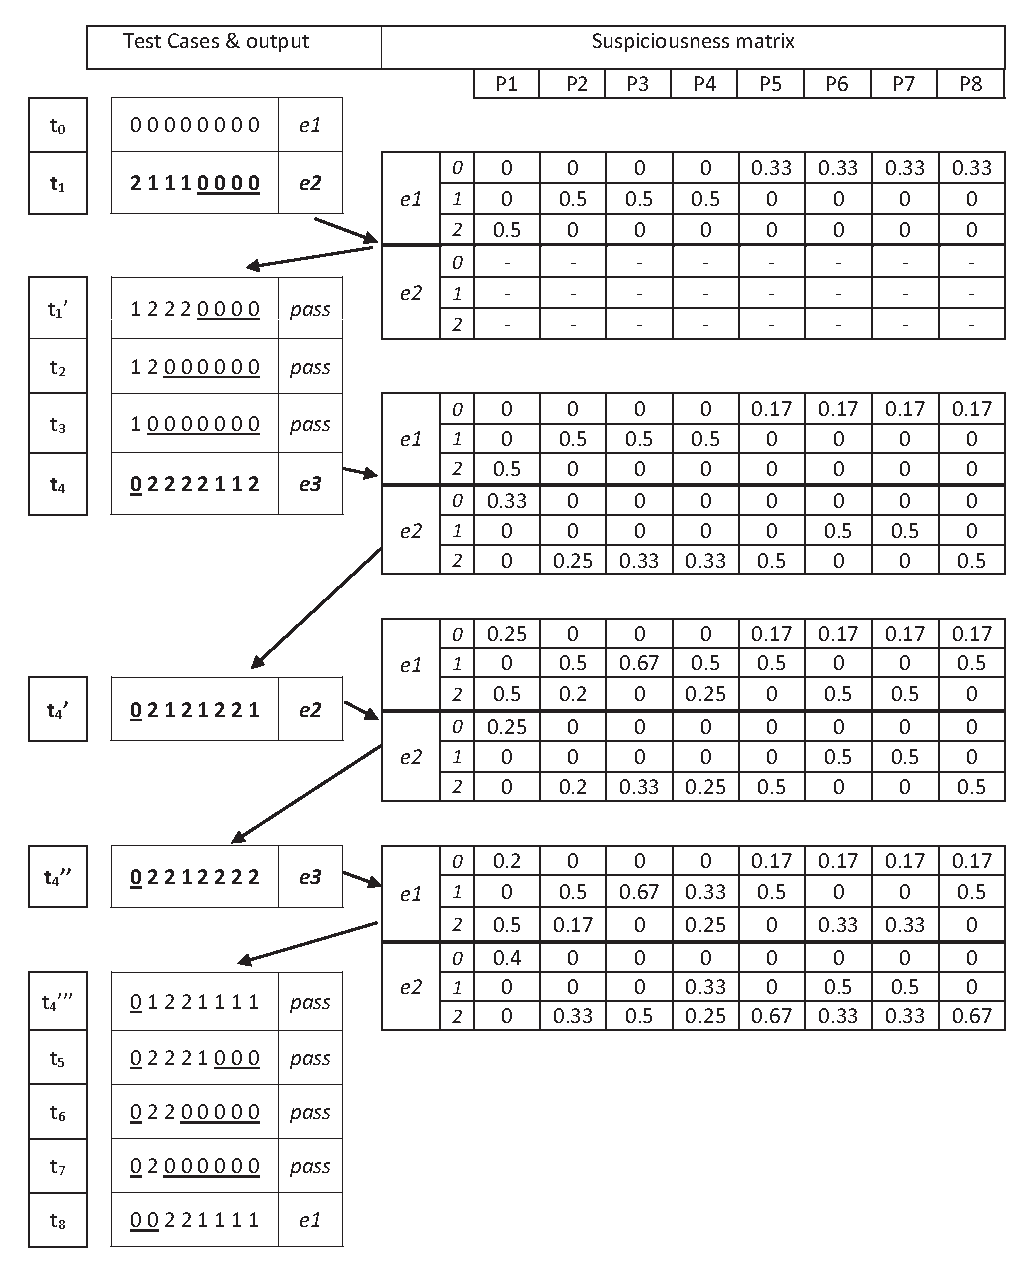
\includegraphics[width=4.31in]{table.eps}
\caption{A case study using our approach}
\label{fig:fci_case_study}
\end{figure}


\subsection{Complexity analysis}
The complexity of our approach relies on two variables: the number of test cases that triggered other failures which need to be replaced, and the number of test cases that need to be tried to generate a non-masking-effect test case. The complexity is the product of these two variables.

The first variable is dependent on the extra test cases that are needed to identify the MFS, and this number varies in different FCI approaches. Table \ref{extra-testcases-complexisty} lists the number of test cases that each algorithm needed to get the MFS, where \emph{d} indicates the number of MFS in the SUT. \emph{k} means the number of the parameters of the SUT. \emph{t} is the degree of MFS in the SUT. \emph{c} is an upper bound, and satisfies $d \leq \frac{c}{2} loglog k$. \emph{v} is the number of values that a parameter can take.

\begin{table}
\centering
\tbl{The number of test cases each FCI approach needed to identify MFS\label{extra-testcases-complexisty}}{
  \begin{tabular}{c | c} \hline
\bfseries Method & \bfseries number of test cases to identify MFS\\ \hline
Charles ELA & depends on the  covering array \\
Martinez with safe value \cite{martinez2008algorithms,martinez2009locating} & $O(\hat{d}log k + \hat{d}^{2})$ \\
Martinez without safe values \cite{martinez2008algorithms,martinez2009locating} & $O(d^{2} + dlog k + log^{c} k)$  \\
Martinez' ELA \cite{martinez2008algorithms,martinez2009locating} &  $O(ds^{v}log k)$\\
Shi SOFOT \cite{shi2005software}& $O(k)$ \\
Nie OFOT \cite{nie2011minimal} & $O(k \times d)$\\
Ylimaz classification tree & depends on the  covering array\\
FIC \cite{zhang2011characterizing} &  $O(k)$ \\
FIC\_BS \cite{zhang2011characterizing}& $O(t(log k + 1) + 1)$\\
Ghandehari's suspicious based  \cite{ghandehari2012identifying}& depends on the number and size of MFS\\
TRT \cite{niu2013identifying}&  $O(d\times t \times log k + t^{d})$\\ \hline
  \end{tabular}
  }
  \end{table}

Note that each algorithm may have some restrictions, details of which are shown in \cite{zhang2011characterizing}.

To get the magnitude of the second variable, we need to figure out the probability of a test case that could trigger other failure. The first consideration is the \emph{fixed} part, as the additional generated test case should somehow contain this part. As mentioned before, we can generate $(v-1)^{k - p} $  (\emph{p} is the number of parameter values in the \emph{fixed} part) possible test cases that contain the \emph{fixed} part. Apart from the one that needs to be replaced, there remain $(v-1)^{k - p}- 1$ candidate test cases, which indicates the complexity is $O((v-1)^{k - p} - 1)$. However, to avoid the exponential computation, we use the $MeetEndCriteria()$ function to end Algorithm 1 when the attempts to find a proper test case is over a prior given constant, say $N$, so the complexity for the second part is $O( min (N, (v-1)^{k - p} - 1))$.
%
%While for adaptive approach, as the $\emph{fixed}$ part is derived from the existed failing test case, which in fact make the test cases to be selected one more less (the existed one), so the complexity is  $O(v^{k - p} - 2)$.

We note that exponent $k - p$ has a significant effect on the complexity of the second value. The greater $p$ is, the less test cases that can be generated. Different approach has different $p$. For example, for the OFOT approach, $p$ is equal to $k - 1$.  And for the FIC\_BS approach, $p$ varies ranging from $k-1$ to $1$. While for the non-adaptive approaches, as the $fixed $ part is commonly the schemas that are needed to be covered, so the $p$ for these approaches is at least equal to $t$. We have listed all of them in Table \ref{fixed-part-complexisty}. It is noted that the approach $Martinez\ without\ safe values$ has no such complexity, because it works when $v = 2$, and this results in not having other test cases to be replaced if we test a fixed part when triggering other failures.

\begin{table}
\centering
\tbl{The complexity of the second part\label{fixed-part-complexisty}}{
  \begin{tabular}{c | c} \hline
\bfseries Method & \bfseries fixed part\\ \hline
Charles ELA &   $O( min (N, (v - 1)^{k - t} - 1))$\\
Martinez with safe value \cite{martinez2008algorithms,martinez2009locating} &$O( min (N, (v-1) - 1)) \sim O( min (N, (v-1)^{k - 1} - 1))$\\
Martinez without safe values \cite{martinez2008algorithms,martinez2009locating} &$ - $  \\
Martinez' ELA \cite{martinez2008algorithms,martinez2009locating} & $O( min (N, (v - 1)^{k - t} - 1))$\\
Shi SOFOT \cite{shi2005software}& $O( min (N, (v-1) - 1))) $\\
Nie OFOT \cite{nie2011minimal} & $O( min (N, (v-1) - 1)))$\\
Ylimaz classification tree & $O( min (N, (v - 1)^{k - t} - 1)$\\
FIC \cite{zhang2011characterizing} &  $O( min (N, (v-1) - 1)) \sim O( min (N, (v-1)^{k - 1} - 1))$\\
FIC\_BS \cite{zhang2011characterizing}& $O( min (N, (v-1) - 1)) \sim O( min (N, (v-1)^{k - 1} - 1))$\\
Ghandehari's suspicious based  \cite{ghandehari2012identifying}&$ O( min (N, (v - 1)^{k - t} - 1))$\\
TRT \cite{niu2013identifying}&$ O( min (N, (v-1) - 1)) \sim O( min (N, (v-1)^{k - 1} - 1)) $\\ \hline
  \end{tabular}
  }
  \end{table}

Above all, the cost of replacement strategy varies in different FCI approaches. Note that this cost is computed for the worst case, and in practice much less test cases are needed to identify the MFS. This is because first, not every test case generated by the FCI approach needs to be replaced; and second, a satisfied test case can usually be found before the whole searching space is explored. From complexity analysis, in fact, we cannot determine which approach is better than others, as the cost of each approach is dependent on different factors. For example in Table \ref{extra-testcases-complexisty}, the extra test cases needed for OFOT\cite{nie2011minimal} and FIC\_BS\cite{zhang2011characterizing} are $O(k \times d)$ and $O(t(log k + 1) + 1)$ , respectively. Values $t$, $k$ and $d$ determine which one is better in practice. So for different SUT with different MFS, which FCI approach is better can be completely changed. Besides, the less cost in practice is not always good for identifying MFS.  A potential problem is, with less candidate test cases, the replacement strategy may not find a satisfied test case, which will result in a low quality of the identified schemas.


%we can find that  the worst is . However, this is not means that it , because the less candidate cases also can give a less chance to get the satisfied test case.  In this paper, we choose the FCI BS as the candidate, because it can probably, and its test cases are less, but, it is not necessary the best, because these approaches has its own restrictions. And in some partucal, For example, if there are overlapped, a better choice is TRT \cite{niu2013identifying}.

%The production of this two complexity is the final complexity for our approach. This result is a upper bond, most times the system will just contain small size of failures which will significantly not reach this bond. Also, if a system with too many bugs that make the replacement too costly will just need to rewrite instead of identifying. Further more our "suspicious set" will largely reduce the replacement cost comparing with previous work, which will be validated in the empirical study later.
%
%This complexity is well lay on the number of failures and the magnitude and location of the MFS of each schema, we only analysis the average performance of our approach. Also this approach also lay on the number of tests need to be executed about each algorithm.


\section{empirical studies}
To investigate the impact of masking effects on FCI approaches in real software testing scenarios and to evaluate the performance of our approach in handling this effect, we conducted several empirical studies. Each of the studies focuses on addressing one particular issue, as follows:

%, the first study survey several real opens-source software to figure out the existence and the characteristics of masking effects in practice, the second study aims to comparing the performance between our augment approach with traditional ones. The third study focus on evaluating the efficiency of the searching technique in our strategy, i.e., the method to find a test case that satisfied our requirement.  The last study aims at comparing the performance of our augment approach with existed masking effects handling approach -- FDA-CIT \cite{yilmaz2013reducing}.

% determining the extent to which that two traditional strategies suffered from the masking effects, the last study focus on evaluating the performance of our approach as well as comparing it with two traditional strategies and previous approach using random replacing selection strategy.

% to figure out the test cases.

%In this section, we conducted several empirical studies to address the following questions:
\textbf{Q1}: Do masking effects exist in real software that contains multiple failures?

\textbf{Q2}: How well does our approach perform compared to traditional approaches?

\textbf{Q3}: Is the ILP-based test case searching technique efficient compared to the random selection?

\textbf{Q4}: Compared to another masking effects handling approach FDA-CIT \cite{yilmaz2013reducing}, does our approach have any advantages ?
%et improvement in handling effects and limiting the costs(reducing extra test cases).

%\textbf{Q5}: Does voting system that consists of different approaches can make improvements?
%
%Specifically, section 6.1 surveyed several open-source software to gain a insight of the existence of multiple failures and their masking effects. Section 6.2 directly applied three MFS-identifying programs on the surveyed software and analysis their results. Section 6.3 applied our approach on the software and a comparison with traditional approaches will be discussed. Section 6.4 discuss the threats to validity of our empirical studies.

\subsection{The existence and characteristics of masking effects}
In the first study, we surveyed two kinds of open-source software systems to gain an insight into the existence of multiple failures and their effects. The software under study were HSQLDB and JFlex. The first is a database management software written in pure Java and the second is a lexical analyser generator. The reason that we chose these two systems is because they both contain different versions and are all highly configurable so that the options and their interactions can affect their behaviour. Additionally, they all have a developer community so that we can easily obtain the real bugs reported in the bug tracker forum. Table \ref{software description} lists the program, the versions surveyed, number of lines of uncommented code, number of classes in the project, and the bug's id \footnote{ http://sourceforge.net/p/hsqldb/bugs \\
http://sourceforge.net/p/jflex/bugs  }for each of the software.

%\begin{table}\renewcommand{\arraystretch}{1.3}
%\caption{Software under survey}
%\label{software description}
%
%\end{table}
%\begin{table}\renewcommand{\arraystretch}{1.3}
%\tbl{Software under survey\label{software description}}{
%\begin{tabular}{c|c|c|c|c} \hline
%software & versions & LOC & classes & bug pairs\footnote{ http://sourceforge.net/p/hsqldb/bugs
%http://sourceforge.net/p/jflex/bugs  } \\ \hline
%
%HSQLDB  &2.0rc8 & 139425 & 495 &  \#981 \& \#1005\\
%	   &2.2.5 & 156066 & 508 & \#1173 \&  \#1179\\
%	    &2.2.9 & 162784 &525 & \#1286 \& \#1280\\
%JFlex  &1.4.1 &  10040 &58 & \#87 \& \#80 \\
%      &1.4.2 &  10745 &61 &  \#98 \& \#93  \\
%\hline\end{tabular}
%}
%\end{table}
\begin{table}\renewcommand{\arraystretch}{1.3}
\tbl{Software under survey\label{software description}}{
\begin{tabular}{c|c|c|c|c} \hline
software & versions & LOC & classes & bug pairs \\ \hline

HSQLDB  &2.0rc8 & 139425 & 495 &  \#981 \& \#1005 \\
	   &2.2.5 & 156066 & 508 & \#1173 \&  \#1179\\
	    &2.2.9 & 162784 &525 & \#1286 \& \#1280\\
JFlex  &1.4.1 &  10040 &58 & \#87 \& \#80 \\
      &1.4.2 &  10745 &61 &  \#98 \& \#93  \\
\hline\end{tabular}
}
\end{table}
%http://hsqldb2.0.sourcearchive.com/downloads/2.0.0$\scriptsize{\sim}$rc8/

%\footnote{http://sourceforge.net/projects/jflex/files/jflex}

% \footnote{http://sourceforge.net/projects/hsqldb/files/hsqldb/ }

\subsubsection{Study setup}
We first looked through the bug tracker forum and focused on the bugs which are caused by the options interactions. For each such bug, we derived its MFS by analysing the bug description report and the associated test file which can reproduce the bug. For example, through analysing the source code of the test file of bug\#981 for HSQLDB, we found the failure-inducing interaction for this bug is (\emph{preparestatement}, \emph{placeHolder}, \emph{Long string}). These three parameter values together form the condition that triggers the bug. The analysed result was later regarded as the ``prior MFS".

We further built the testing scenario for each version of the software listed in Table \ref{software description}. The testing scenario is constructed so that we can reproduce different failures by controlling the inputs to the test file. For each version, the source code of the testing file as well as other detailed information is available at https://code.google.com/p/merging-bug-file.

Next, we built the input model which consists of the options related to the failure-inducing interactions and additional options that are commonly used. The detailed model information is shown in Tables \ref{modelHSQLDB} and \ref{modelJFlex} for HSQLDB and JFLex, respectively. Each table is organised into three groups: (1) \emph{common options}, which lists the options as well as their values under which every version of this software can be tested; (2) \emph{specific options}, under which only the specific version can be tested; and (3) \emph{configure space}, which depicts the input model for each version of the software, presented in the abbreviated form $\#values^{\#number\ of\ parameters} \times ...$, e.g., $2^{9} \times 3^{2} \times 4^{1}$ indicates the software has 9 parameters that can take 2 values, 2 parameters 3 values, and only one parameter 4 values.

\begin{table}[h]
\tbl{Input model of HSQLDB\label{modelHSQLDB}}{
\begin{tabular}{llllll}
  \hline
\multicolumn{3}{c}{\bfseries common options} & \multicolumn{3}{c}{\bfseries values}  \\
  \hline
 \multicolumn{3}{c}{Server Type} & \multicolumn{3}{c}{server, webserver, inprocess}  \\
  \multicolumn{3}{c}{  existed form}  & \multicolumn{3}{c}{mem, file}  \\
   \multicolumn{3}{c}{ resultSetTypes}  & \multicolumn{3}{c}{forwad, insensitive, sensitive} \\
   \multicolumn{3}{c}{ resultSetConcurrencys}  & \multicolumn{3}{c}{read\_only, updatable}  \\
  \multicolumn{3}{c}{  resultSetHoldabilitys}  &\multicolumn{3}{c}{ hold, close} \\
  \multicolumn{3}{c}{ StatementType }  &\multicolumn{3}{c}{statement, prepared}  \\
  \multicolumn{3}{c}{ sql.enforce\_strict\_size}  & \multicolumn{3}{c}{true, false}  \\
  \multicolumn{3}{c}{  sql.enforce\_names}  &\multicolumn{3}{c}{ true, false} \\
  \multicolumn{3}{c}{ sql.enforce\_refs }  &\multicolumn{3}{c}{true, false}  \\
    \hline
%   \multicolumn{6}{c}{  \bfseries common Boolean options }\\
%    \hline
%    \multicolumn{6}{c}{   sql.enforce\_strict\_size, sql.enforce\_names, sql.enforce\_refs}\\
%      \hline
   \bfseries versions &   \multicolumn{2}{c}{  \bfseries specific options}  & \multicolumn{3}{c}{  \bfseries values}\\
     \hline
    2.0rc8 & \multicolumn{2}{c}{ more} & \multicolumn{3}{c}{ true, false}\\
      & \multicolumn{2}{c}{ placeHolder} & \multicolumn{3}{c}{ true, false }\\
      & \multicolumn{2}{c}{ cursorAction }& \multicolumn{3}{c}{ next,previous,first,last}\\
    2.2.5 &\multicolumn{2}{c}{  multiple} & \multicolumn{3}{c}{ one, multi, defailure}\\
       & \multicolumn{2}{c}{ placeHolder} & \multicolumn{3}{c}{ true, false}\\
    2.2.9 & \multicolumn{2}{c}{ duplicate }& \multicolumn{3}{c}{ dup, single, defailure}\\
     & \multicolumn{2}{c}{ defailure\_commit} & \multicolumn{3}{c}{ true, false} \\
        \hline
   \bfseries versions &  \multicolumn{3}{c}{\bfseries Config space}&\multicolumn{2}{c}{}\\
   \hline
   2.0rc8 & \multicolumn{3}{c}{$2^{9} \times 3^{2} \times 4^{1}$} &\multicolumn{2}{c}{} \\
    2.2.5 &  \multicolumn{3}{c}{$2^{8} \times 3^{3}$ } & \multicolumn{2}{c}{} \\
     2.2.9 & \multicolumn{3}{c}{$2^{8} \times 3^{3}$} &\multicolumn{2}{c}{} \\ \hline
\end{tabular}
}
\end{table}

\begin{table}[h]
\tbl{Input model of JFlex\label{modelJFlex}}{
\begin{tabular}{llllll}
  \hline
\multicolumn{3}{c}{\bfseries common options} & \multicolumn{3}{c}{\bfseries values}  \\
  \hline

 \multicolumn{3}{c}{ generation} & \multicolumn{3}{c}{switch, table, pack}  \\
  \multicolumn{3}{c}{  charset}  & \multicolumn{3}{c}{default, 7bit, 8bit, 16bit}  \\

   \multicolumn{3}{c}{ public} & \multicolumn{3}{c}{true, false}  \\
  \multicolumn{3}{c}{  apiprivate}  & \multicolumn{3}{c}{true, false}  \\
   \multicolumn{3}{c}{ cup} & \multicolumn{3}{c}{true, false}  \\
      \multicolumn{3}{c}{ caseless} & \multicolumn{3}{c}{true, false}  \\
  \multicolumn{3}{c}{  char}  & \multicolumn{3}{c}{true, false}  \\
   \multicolumn{3}{c}{ line} & \multicolumn{3}{c}{true, false}  \\
  \multicolumn{3}{c}{  column}  & \multicolumn{3}{c}{true, false}  \\
     \multicolumn{3}{c}{ notunix} & \multicolumn{3}{c}{true, false}  \\
  \multicolumn{3}{c}{  yyeof}  & \multicolumn{3}{c}{true, false}  \\

    \hline
%   \multicolumn{6}{c}{  \bfseries common boolean options }\\
%    \hline
%    \multicolumn{6}{c}{ public, apiprivate,cup,caseless,char,line,column,notunix, yyeof}\\
%      \hline

   \bfseries versions &   \multicolumn{2}{c}{  \bfseries specific options}  & \multicolumn{3}{c}{  \bfseries values}\\
     \hline
    1.4.1 & \multicolumn{2}{c}{ hasReturn} & \multicolumn{3}{c}{ has, non, default}\\
      & \multicolumn{2}{c}{ normal} & \multicolumn{3}{c}{ true, false }\\
    1.4.2 &\multicolumn{2}{c}{ lookAhead} & \multicolumn{3}{c}{one, multi, default}\\
       & \multicolumn{2}{c}{ type} & \multicolumn{3}{c}{ true, false}\\
     & \multicolumn{2}{c}{ standalone }& \multicolumn{3}{c}{true, false}\\

        \hline
   \bfseries versions &  \multicolumn{3}{c}{\bfseries Config space}&\multicolumn{2}{c}{}\\
   \hline
  1.4.1  & \multicolumn{3}{c}{$2^{10} \times 3^{2} \times 4^{1} $} &\multicolumn{2}{c}{} \\
   1.4.2 &  \multicolumn{3}{c}{$2^{11} \times 3^{2} \times 4^{1} $ } & \multicolumn{2}{c}{} \\ \hline
\end{tabular}
}
\end{table}

We then generated the exhaustive set of test cases consisting of all possible interactions of these options. For each of them, we executed the prepared testing file. We recorded the output of each test case to observe whether there were test cases containing prior MFS that did not produce the corresponding bug. Later we refer to those test cases that contain the MFS but did not trigger the expected failure as the \emph{masked} test cases.

%Then we collected the bugs that belong to one same version. It is naturally that the more bugs we collect for one version, the masking effects will more likely to be triggered in that software of the particluar version. Table \ref{statitstics_of_bugs} lists the result we collected. This table in turns provides the software name, the particular version and the number of bugs we have found in the bug tracker. The last column presents the number of pairs of bugs that can conflict with each other, i.e., these pairs of bugs cannot appear in one test case, such that they cannot mask each other.
%
%\begin{table}\renewcommand{\arraystretch}{1.3}
%\tbl{The bugs statistics of the software\label{statitstics_of_bugs}}{
%\begin{tabular}{c|c|c|c} \hline
%software & versions & Num of bugs & conflict number\\ \hline
%
%HSQLDB  &2.0rc8 & 139425 & 495 \\
%	   &2.2.5 & 156066 & 508 \\
%	    &2.2.9 & 162784 &525 \\
%JFlex  &1.4.1 &  10040 &58\\
%      &1.4.2 &  10745 &61 \\
%\hline\end{tabular}
%}
%\end{table}



%
%When two bugs conflict each other (cannot appear in one test case)
%
%1.possible situation, the 1 version, and the failures that are found in this version, and the possible failures can be .
%

\subsubsection{Results and discussion}

Table \ref{masking effect condition} lists the results of our survey. Column ``all tests" gives the total number of test cases executed.  Column ``failure" indicates the number of test cases that failed during testing, and column ``masking" indicates the number of masked test cases.  The percentage in the parentheses indicates the proportion of masked test cases and the failing test cases.

%[!ht]
\begin{table}\renewcommand{\arraystretch}{1.3}
\tbl{Number of failures and their masking effects\label{masking effect condition}}{
\begin{tabular}{c|c|c|c|c} \hline
software & versions & all tests & failure & masking\\ \hline
HSQLDB & 2cr8 & 18432 & 4608 & 768 (16.7\%)\\ \hline
     - & 2.2.5 & 6912 & 3456 & 576 (16.7\%)\\ \hline
     - & 2.2.9 & 6912 & 3456 &1728 (50\%)\\ \hline
JFlex & 1.4.1 & 36864 & 24576 &6144 (25\%)\\ \hline
     -& 1.4.2 & 73728 & 36864 &6144 (16.7\%)\\ \hline
\end{tabular}
}
\end{table}

We observed that for each version of the software under analysis listed in Table \ref{masking effect condition}, test cases with masking effects do exist, i.e., test cases containing MFS did not trigger the corresponding bug. In fact, there are about 768 out of 4608 test cases (16.7\%) in hsqldb with 2rc8 version. This rate is about 16.7\%, 50\%, 25\%, and 16.7\%, respectively, for the remaining software versions.

So the answer to \textbf{Q1} is that in practice, when SUT have multiple failures, masking effects do exist widely in the test cases.

It is notable that in Yilmaz's \cite{yilmaz2013reducing} paper, a similar study about the existence of the masking effects has been conducted. The main difference between that work and ours is that Yilmaz's work quantify impact of the masking effects as the number of $t$-degree schemas that only appear in the test cases that triggered other failures. Here, the $t$-degree schemas can be either MFS or not. Our work, however, quantify the masking effects as the number of test cases that are masked by unexpected failures. These test cases should contain some MFS, i.e., they should have triggered the expected failure if they did not trigger any other failure.  The reason that we quantify the masking effects in such way is because our work seeks to handle the masking effects in the MFS identifying process. As the test cases which contain the MFS but do not produce the corresponding failure will significantly affect the MFS identifying results, their number can better reflect the impact of the masking effects on the FCI approach.

\subsection{Comparing our approach with traditional algorithms}
The second study aims to compare the performance of our approach with traditional approaches in identifying MFS under the impact of masking effects. To conduct this study, we need to apply our approach and traditional algorithms to identify MFS in a  variety of software and evaluate their results. The five versions of software in Table \ref{software description} used as test objects are far from the requirement for a general evaluation. However, to construct many real testing objects is time-consuming as we must carefully study the detail of that software as well as the bug tracker report.  To compromise, we synthesized 10 more testing objects. These synthesized objects are ten small programs which can directly return outputs when executed with given inputs.  To make the synthetic objects as similar as possible to the real software, we firstly analysed the characterizations, such as the number of parameters, the number of failures, and the possible masking effects, of the real software. We observed that the number of parameters of the SUT ranged from 8 to 30, the number of different failures in the SUT ranged from 2 to 4, and the number of MFS for a failure ranged from 1 to 2, in which the degree of the MFS ranged from 1 to 6. Then for each characterization, we randomly selected one value in the corresponding range and assigned it to the input model by adjusting the relationships between the inputs and outputs of these programs.

Table \ref{testing_models} lists the testing model for both the real and synthesizing testing objects. In this table, column `Object' indicates the SUT under test. For the real SUT listed in Table \ref{software description}, we label the five software as $H2cr8$, $H2.2.5$, $H2.2.9$, $J1.4.1$, $J1.4.2$, respectively. While for the synthesized ones, we label them in the form of `\emph{syn}+ \emph{id}'. Column `Model' presents the input space for each testing object. Column 'Failures' shows the different failures in the software and their masking relationships. In this column, `$>$' means the left failure will mask the right failure, i.e., if the left failure is triggered, then the right failure will not be triggered. Furthermore, '$>$' is transitive so that the left failure can mask all the failures in the right.  For example, for the $H2cr8$ object, we can find three failures : $e_{1}$, $e_{2}$, and $e_{3}$. By using the formula $e_{1} > e_{2} > e_{3}$, we indicate that the failure $e_{2}$ will mask $e_{3}$ and $e_{1}$ will mask both $e_{2}$ and $e_{3}$. Here for the simplicity of the experiment, we did not build more complex testing scenarios such as the masking effects can happened in the form $e_{1} > e_{2},\ e_{2} > e_{3},\ e_{3} > e_{1}$ or even $e_{1} > e_{2},\ e_{2} > e_{1}$. The last column shows the MFS for each failure. The MFS is presented in an abbreviated form $\{\#index_{\#value}\}_{failure}$, e.g., for the object $H2cr8$, $(5_{1},6_{0},7_{0})_{e_{1}}$ actually means (-, -, -, -, -, 1, 0, 0, -, -, -, - ) is the MFS for the failure $e_{1}$.

\begin{table}\renewcommand{\arraystretch}{1.3}
\tbl{The testing models used in the case study\label{testing_models}}{
\setlength\tabcolsep{1pt}
\begin{tabular}{c|c|c|c} \hline
Object & Model & Failures & MFS for each failure\\ \hline
H2cr8 & $2^{9} \times 3^{2} \times 4^{1}$ & $e_{1} > e_{2} > e_{3} $ & $ (5_{1},6_{0},7_{0})_{e_{1}}, (5_{1},8_{2},9_{2})_{e_{2}} , (5_{1},8_{2},9_{1})_{e_{2}}, (5_{1},8_{3},9_{2})_{e_{3}}, (5_{1},8_{3},9_{1})_{e_{3}}$ \\ \hline
H2.2.5 & $2^{8} \times 3^{3}$ & $ e_{1} > e_{2}$ & $ (6_{1},7_{0})_{e_{1}}, (5_{2})_{e_{2}}$ \\ \hline
H2.2.9 & $2^{8} \times 3^{3}$& $e_{1} > e_{2} > e_{3}$ & $ (6_{0})_{e_{1}}, (0_{1},5_{1},7_{0})_{e_{2}} , (0_{0},5_{1},7_{0})_{e_{2}} , (5_{1},7_{0})_{e_{3}} $ \\ \hline
J1.4.1 & $2^{10} \times 3^{2} \times 4^{1}$& $ e_{1} > e_{2} $ &$(0_{0})_{e_{1}}, (1_{0})_{e_{2}} $ \\ \hline
J1.4.2 & $2^{11} \times 3^{2} \times 4^{1}$& $e_{1} > e_{2}$ &$(1_{0},2_{1})_{e_{1}}, (0_{1})_{e_{2}}  $\\ \hline
syn1 & $2^{5}\times 3^{3}\times 4^{1}$& $e_{1} > e_{2}$ &$ (2_{1},3_{0})_{e_{1}}, (1_{1},2_{1})_{e_{2}} , (1_{0},3_{0})_{e_{2}}$ \\ \hline
syn2 & $2^{6}\times 3^{2}\times 4^{1}$ & $e_{1} > e_{2} > e_{3} $ &$ (4_{1},6_{0},7_{1},8_{0})_{e_{1}}, (1_{1},3_{1},5_{1})_{e_{2}}, (2_{0},3_{1},6_{0})_{e_{3}} $\\ \hline
syn3 & $2^{5}\times 3^{3}$ & $e_{1} > e_{2} > e_{3}$ &$ (2_{1},3_{0})_{e_{1}},  (1_{0})_{e_{2}}, (4_{1})_{e_{2}}, (6_{0},7_{0})_{e_{3}} $\\ \hline
syn4 & $2^{7}\times 3^{2}\times 4^{1}$ & $e_{1} > e_{2} > e_{3}$ &$ (0_{1},2_{1},5_{0},6_{1})_{e_{1}}, (2_{1},4_{0})_{e_{2}}, (6_{1},7_{0})_{e_{2}}, (3_{0},4_{0},5_{0})_{e_{3}} $\\ \hline
syn5 & $2^{4}\times 3^{3} \times 4^{2}$ & $e_{1} > e_{2}$ &$ (0_{0},1_{1},3_{0},6_{1},8_{0})_{e_{1}}, (2_{0},3_{0},4_{1})_{e_{2}}$\\ \hline
syn6 & $2^{9}\times 3^{2}$ & $e_{1} > e_{2} > e_{3} > e_{4}$ &$  (2_{0},7_{1},8_{1})_{e_{1}}, (3_{1},5_{1})_{e_{2}} , (4_{0})_{e_{2}}, (3_{1},6_{0},7_{1})_{e_{3}}, (3_{1},7_{1},8_{0})_{e_{4}}$ \\ \hline
syn7 & $2^{10}\times 3^{1}\times 4^{1}$&$e_{1} > e_{2} > e_{3}$ &$ (3_{1},4_{0},5_{0})_{e_{1}}, (2_{0}, 4_{0}, 7_{1},9_{0})_{e_{2}}, (6_{1},10_{0},11_{1})_{e_{3}} $ \\ \hline
syn8 & $2^{11}\times 3^{1}\times 4^{1}$& $e_{1} > e_{2} $ &$ (1_{0},3_{1},4_{0},7_{1},9_{0},12_{1})_{e_{1}}, (0_{0},2_{1},3_{1},7_{1},10_{0},11_{1})_{e_{2}} $\\ \hline
syn9 & $2^{4}\times 4^{3}$ & $e_{1} > e_{2}$ & $(3_{1},5_{0})_{e_{1}}, (5_{0},6_{1})_{e_{2}} $ \\ \hline
syn10 & $2^{7}\times 3^{3} \times 4^{1}$ & $e_{1} > e_{2}$ &$ (0_{1},3_{0},4_{1},7_{0})_{e_{1}},   (2_{0},3_{0},5_{1})_{e_{2}}, (2_{0},3_{0},5_{0})_{e_{2}} $\\ \hline
\end{tabular}
}
\end{table}


\subsubsection{Study setup}
After preparing the objects under testing, we then applied our approach (FIC\_BS with replacement strategy) to identify the MFS. Specifically, for each SUT we selected each test case that failed during testing and fed it into our FCI approach as the input. Then, after the identifying process was completed, we recorded the identified MFS and the extra test cases needed. For the traditional FIC\_BS approach, we designed the same experiment. But as the objects being tested have multiple failures for which the traditional FIC\_BS can not be applied directly, we adopted two traditional strategies on the FIC\_BS algorithm, i.e., \emph{regarded as one failure} and \emph{distinguishing failures} as described in Section 3.2.  The purpose of recording the generated additional test cases is to quantify the additive cost of our approach.

We next compared the identified MFS of each approach with the prior MFS to quantify the degree that each suffers from masking effects. There are five metrics used in this study, listed as follows:
 \begin{enumerate}
 \item \emph{Accurate number} : the number of identified MFS which are actual prior MFS.
 \item \emph{Super number}: the number of identified MFS that are the super schemas of some prior MFS.
 \item \emph{Sub number} : the number of identified MFS that are the sub schemas of some prior MFS.
 \item  \emph{Ignored number} : the number of schemas that are in the prior MFS, but irrelevant to the identified MFS.
 \item \emph{Irrelevant number} : the number of schemas in the identified MFS that are irrelevant to the prior MFS.
\end{enumerate}

Among these five metrics, the \emph{accurate number} directly indicates how effectively the FCI approaches performed, since to identify as many actual MFS as possible is the target for every FCI approach.  Metrics \emph{ignored number} and \emph{irrelevant number} indicate the extent of deviation for the FCI approaches, specifically, the former indicates how much information about the MFS will miss, while the latter indicates how serious the distraction would be due to the useless schemas identified by the FCI approach.  \emph{Super number} and \emph{sub number} are the metrics in between, i.e., to identify some schemas that is \emph{super} or \emph{sub} schemas of the actual MFS is better than identifying \emph{irrelevant} ones or ignoring some MFS, but it is worse than identifying the schema that is identical to some actual MFS. This is intuitive, as given the \emph{super} / \emph{sub} schemas, we just need to \emph{remove} / \emph{add} some elements of the original schemas to get the actual MFS.  While for the \emph{irrelevant} or \emph{ignore} ones, however, more efforts will be needed (e.g., both \emph{adding} and \emph{removing} operations will be needed to revise the irrelevant schemas to the actual MFS).

Besides these specific metrics, we also give a composite metric to measure the overall performance of each approach. The composite metric \emph{aggregate} is defined as follows:

$$ Aggregate =  \frac{accurate + related(super) + related(sub)}{accurate + super + sub + irrelevant + ignored} $$

In this formula, \emph{accurate, super, sub, irrelevant, } and \emph{ignored} represent the value of each specific metric. To refine the evaluation of different \emph{super} / \emph{sub} schemas, we design a \emph{related} function which gives the similarity between the schemas (either super or sub) and the real MFS, so that we can quantify the specific effort for changing a \emph{super} / \emph{sub} schema to the real MFS. The similarity between two schemas $S_{A}$ and $S_{B}$ is computed as:

\begin{displaymath} Similarity(S_{A},S_{B})= \frac{number\ of\ same\ elements\ in\ S_{A}\ and\ S_{B}}{\max (Degree(S_{A}),Degree(S_{B})) } \end{displaymath}.

For example, the similarity of  (- 1\ 2 - 3) and  (- 2\ 2 - 3) is $\frac{2}{3}$. This is because $S_{A}$ and $S_{B}$ have the same third and last elements, and both of them are three-degree.

So the \emph{related} function is the summation of similarity of all the super or sub schemas with their corresponding MFS.

\subsubsection{Results and discussion}

 \begin{figure*}[htbp]
%\centering
\subfigure[Result of the number of accurately identified MFS]{
  %  \rule{4cm}{3cm}
    \label{fig:21}
    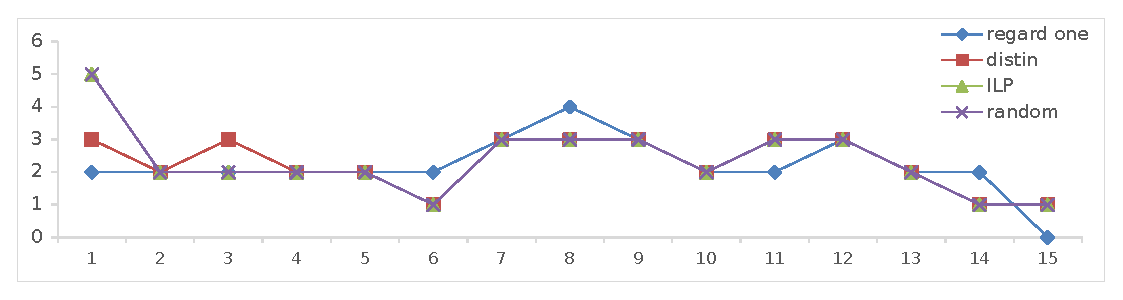
\includegraphics[width=2.64in]{accurate.eps}
}
\subfigure[Result of the number of identified sub-schemas of the MFS]{
  %  \rule{4cm}{3cm}
    \label{fig:22}
    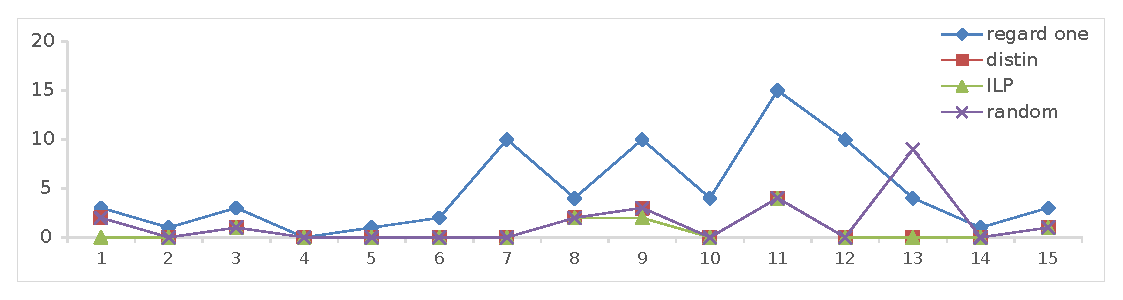
\includegraphics[width=2.64in]{sub.eps}
}
\subfigure[Result of the number of identified super-schemas of the MFS]{
  %  \rule{4cm}{3cm}
    \label{fig:23}
    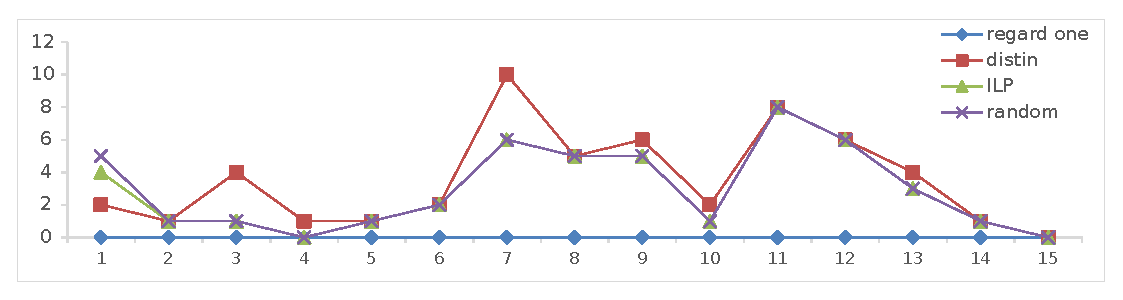
\includegraphics[width=2.64in]{parent.eps}
}
\subfigure[Result of the number of ignored MFS]{
  %  \rule{4cm}{3cm}
    \label{fig:24}
    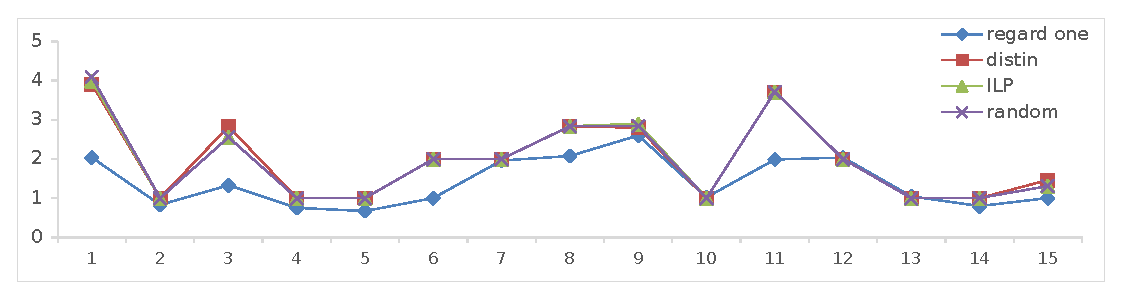
\includegraphics[width=2.64in]{ignore.eps}
}
\subfigure[Result of the number of identified irrelevant schemas of the MFS]{
  %  \rule{4cm}{3cm}
    \label{fig:25}
    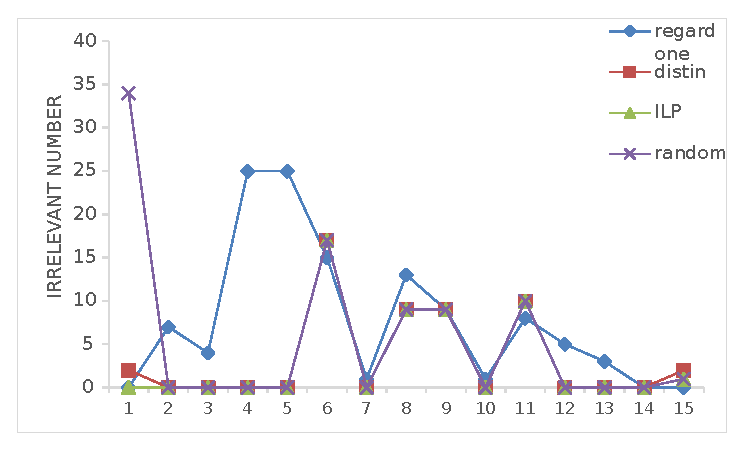
\includegraphics[width=2.64in]{irrelevant.eps}
}
\subfigure[The aggregative result for the five metrics]{
  %  \rule{4cm}{3cm}
    \label{fig:26}
    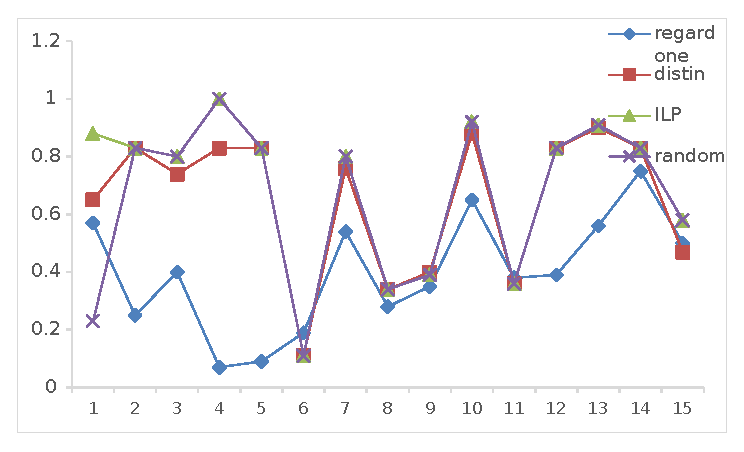
\includegraphics[width=2.64in]{overall.eps}
}
\subfigure[Needed test cases]{
  %  \rule{4cm}{3cm}
    \label{fig:27}
    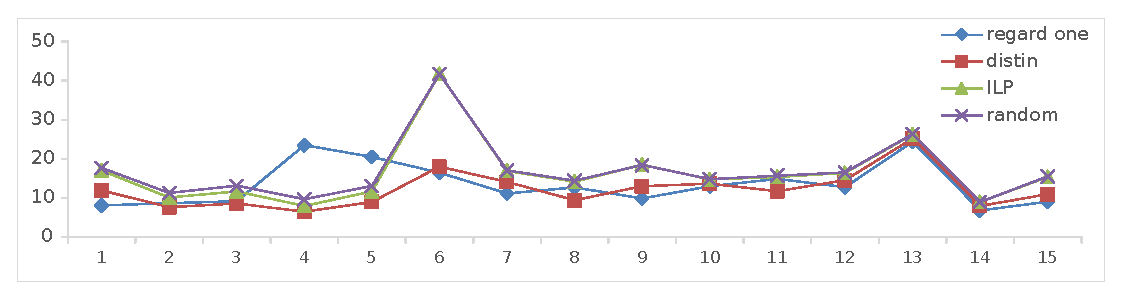
\includegraphics[width=2.64in]{testCases.eps}
}
\caption[Optional caption for list of figures]{Result of the evaluation of each approach}
\label{fig:comparetotraditional}
\end{figure*}


% Table generated by Excel2LaTeX from sheet 'Sheet1'

 Figure \ref{fig:comparetotraditional} depicts the results of the second case study. There are seven sub-figures in this figure, i.e., Figure \ref{fig:21} to Figure \ref{fig:27}. They indicate the results of the number of accurate MFS each approach identified, the number of identified schemas which are the sub-schema / super-schema of some prior MFS, the number of ignored prior MFS, the number of identified schemas which are irrelevant to all the prior MFS, the aggregate value, and the extra test cases each algorithm needed, respectively. For each sub-figure, there are four polygonal lines, each of which shows the results for one of the four strategies: \emph{regarded as one failure}, \emph{distinguishing failures},  \emph{replacement strategy based on ILP searching},  \emph{replacement strategy based on random searching} (The last one will be discussed in the next case study). Specifically, each point in the polygonal line indicates the specific result of a particular strategy for the corresponding testing object. For example in Figure \ref{fig:21}, the point marked with `$\blacklozenge$' at (1,2) indicates that the approach using \emph{regarded as one failure} strategy identified 2 accurate MFS in the testing object--HSQLDB 2cr8. The raw data for this experiment can be found in Table \ref{evaluation_all} of the Appendix. Note that all the data except for the metric \emph{ignored number} are based on all failing test cases for each testing object, i.e., we got the data by comparing the union of the schemas identified in each the failing test cases to the prior actual MFS. As for metric \emph{ignored number}, however, we found that if we merged all the schemas identified in each failing test case, there is no MFS ignored. We therefore use the average score of \emph{ignored number} for each failing test case, which can be seen in the parentheses in Column \emph{ignore} of Table \ref{evaluation_all}.  Next we will discuss the results for each metric.


\textbf{Accurate number: }
Figure \ref{fig:21} shows the number of accurate schemas that each approach achieved.  It appears that there is no outstanding strategy, i.e., there does not exist a strategy that can always perform better or worse than others. For example, for the testing object 1, \emph{ILP} performed the best in obtaining the accurate MFS, while for the testing object 2, \emph{distinguishing failures} identified the most accurate MFS and for testing object 3, \emph{regarded as one failure} did the best. However, upon closer inspection, we can find that strategy \emph{distinguishing failures} performed a little better than strategy \emph{regarded as one failure}. This can be reflected in that there are four testing objects (1, 3, 11, and 15) on which strategy \emph{distinguishing failures} performed better, while for strategy \emph{regarded as one failure} there are only three superior testing objects (6, 8, and 14). This subtle difference can be explained by our formal analysis in Section 4. Specifically, for the strategy \emph{regarded as one failure}, only rule 1 in Table \ref{fci_mask_regard} can result in the FCI approaches identifying the schemas that are identical to some actual MFS, while for \emph{distinguishing failures}, there are two rules (rule 1 and 6a in Table \ref{fci_mask_distinguish}). As a result, \emph{distinguishing failures} strategy has a slighter larger chance than \emph{regard as one failure} to identify the schemas that are identical to the actual MFS.


We can further find that strategies \emph{replacement strategy based on ILP searching} (short for \emph{ILP}
later) and \emph{distinguishing failures} have similar results. This can be easily understood, as strategy \emph{ILP} is actually a refinement version of the strategy \emph{distinguishing failures}, which also make the failures distinguished with each other. The main difference between \emph{ILP} and \emph{distinguishing failures} is that the former has to replace the test cases that triggered any failure other than the currently analysed one while the latter will not change the generated test cases. As a result, the comparison of other metrics ( sub, super, ignore, irrelevant numbers) also showed the similarity between strategy \emph{ILP} and \emph{distinguishing failures}.

\textbf{Sub number \& super number: }
Figure \ref{fig:22} and \ref{fig:23} depicts the results for \emph{sub number} and \emph{super number}, respectively. These two figures firstly showed a clear trend for strategies \emph{regarded as one failure} and \emph{distinguishing failures}, i.e., the former identified more sub schemas of actual MFS than the latter, while the latter identified more super schemas of actual MFS than the former. This is consistent with our formal analysis. Specifically, there are 6 rules (rules 2, 4a, 5, 6, 8a, 9a listed in Table \ref{fci_mask_regard}) for  strategy \emph{regarded as one fault} that can lead to the identified schemas being sub schemas of actual MFS, while \emph{distinguishing failures} strategy has 2 such rules (rules 5, 6c  in Table \ref{fci_mask_distinguish}). But for the rules that can result in the schemas being super schemas of actual MFS, strategy \emph{regarded as one failure} only has one (rule 3 in Table \ref{fci_mask_regard}), while \emph{distinguishing failure} has 5 such rules (rules 2, 3, 4, 6b, 8a in Table \ref{fci_mask_distinguish}).

Although offering similar result as \emph{distinguishing failures} strategy, our strategy \emph{ILP} tend to identify fewer sub schemas and super schemas of actual MFS than strategy \emph{distinguishing failures} (testing objects 1, 9 in Figure \ref{fig:22} and testing objects 3, 4,7,9,10 13 in Figure \ref{fig:23}). We believe this is an improvement, as too many sub schemas and super schemas will make it harder to identify the actual MFS. One issue is the redundancy problem, as many sub or super schemas in fact point to the same actual MFS.

\textbf{Ignore number \& irrelevant number: }
The results of the two negative performance metrics are given in Figure \ref{fig:24} and \ref{fig:25}, respectively.

There are two main observations: first, for strategies \emph{regarded as one failure} and \emph{distinguishing failures}, we can find that the former identified more irrelevant schemas of the actual MFS, while the latter ignored more actual MFS. This observation is as expected, because in our formal analysis the strategy \emph{regarded as one failure} has more rules than \emph{distinguish failures} that can lead to the schemas being irrelevant to the actual MFS, in detail, the former has 4 such rules (rules 4b, 7, 8b, 9b in Table \ref{fci_mask_regard} ) while the latter has three (rules 6d, 7,8b in Table \ref{fci_mask_distinguish}).  And for strategy \emph{distinguish failures}, rule 9 in Table \ref{fci_mask_distinguish} increases the chance to ignore the actual MFS than the strategy \emph{regarded as one failure}.

The second observation is that \emph{ILP} did a good job at reducing the scores for these two negative metrics. Specifically, for \emph{ignored number}, our approach performed better than strategy \emph{distinguishing failures} at testing object 3 and 15 in Figure \ref{fig:24}, but is not as good as strategy \emph{regarded as one failure}. In fact, strategy \emph{regarded as one failure} has a significant advantage at reducing the number of ignored MFS as it tends to associate the failures with all the failing test cases. However, when we consider the \emph{irrelevant number}, we can find that our approach is the best among all three strategies ( better than \emph{distinguishing failures} at testing object 1 in Figure \ref{fig:25}, and better than strategy \emph{regarded as one failure} for  most testing objects) . We believe this improvement is caused by our test cases replacing strategy, as it can increase the test cases that are useful for identifying the MFS and decrease those useless test cases.


\textbf{Aggregative for the five metrics: }
The composite results are given in Figure \ref{fig:26}. This metric gives an overall evaluation of the quality of the identified schemas. From this figure, we can find that \emph{ILP} performed the best, next the \emph{distinguishing failures}, the last is the \emph{regarded as one failure} (See the testing object 1, 3 and 4 in Figure \ref{fig:26}).

It is as expected  that \emph{ILP} performed better than \emph{distinguishing failures} as it is actually the refinement version of latter. It is a bit of surprise to find, however, that strategy \emph{distinguishing failures} performed better than \emph{regarded as one failure} at almost all the testing objects. This result cannot be derived from the formal analysis. A possible explanation is that in these testing objects constructed, the possibility of triggering a masking effect is relatively small. Consequently if we take the strategy \emph{regarded as one failure}, we are more likely to misjudge a test case which triggered other failures to be the failing test case for the failure we currently focus on.

\textbf{Test cases: }
 The number of test cases generated for identifying the MFS indicates the cost of FCI approach. The result is listed in Figure \ref{fig:27}.  We can obviously find that strategy \emph{ILP} generated more test cases than the other strategies. In specific, the gap between the \emph{ILP} and other two strategies ranged from about 2 to 5 (except for the 6th testing object, which exceeds 20), this is acceptable when comparing to all the test cases that each approach needed. The increase in test cases for our approach is necessary, as additional test cases must be generated when some test cases are not satisfied for identifying the MFS of the currently analysed failure.  As for strategies \emph{distinguishing failures} and \emph{regarded as one failure}, there is no significant difference between  the number of test cases generated.


Above all, we draw three conclusions, which help to answer \textbf{Q2}:

1) The results of strategy \emph{distinguishing failures} and \emph{regard one failure} are consistent with the previous formal analysis.

2) Considering the quality of the MFS each approach identified, we can find that our \emph{ILP} approach achieves the best performance, followed by the strategy \emph{distinguishing failures}.

3) Although our approach need more test cases than the other two strategies, it is an acceptable number.

 %the answer we got for \textbf{Q2} is that: our approach achieves better performance than two traditional strategies when handling masking effects at an acceptable % extra cost.

\subsection{Evaluating the ILP-based test case searching method}
The third empirical study aims to evaluate the efficiency of the ILP-based test case searching component of our approach. To conduct this study, we implemented an FCI approach which is also augmented by the \emph{replacing test cases} strategy, but the test case is randomly replaced.

%observe the performance of our approach and compare it with the result got by the traditional approaches. Our approach augments the three traditional FCI approaches with replacing test cases strategy described in Section 4.
%, and then we applied these augmented approaches to identify the failure-inducing combinations in the prepared subjects.

\subsubsection{Study setup}
The setup of this case study is based on the second case study, and uses the same SUT model as shown in Table \ref{testing_models}. We apply the new random searching based FCI approach to identify the MFS in the prepared SUTs. To avoid the bias coming from the randomness, we repeat the new approach 30 times to identify the MFS in each failing test case. We then compute the average additional test cases as well as other metrics listed in section 6.2.1 for the random-based approach.

% We will also take a look at how many scores can the new approach get when measuring the aforementioned metrics, as the same, we just compare the average scores with traditional ones.
%Additionally, comparisons between the augmented approaches and three traditional ones will be quantified.

\subsubsection{Results and discussion}
The evaluation of this random-based approach is also shown in Figure \ref{fig:comparetotraditional}, in which the polygonal line marked with  '$\times$' in each sub-figure indicates the results. The raw data can also be found in the column 'R' of Table \ref{evaluation_all} in the appendix.

Compared to the ILP-based approach, we can firstly observe that there is little distinction between them in terms of the metrics: accurate schemas, super-schemas, sub-schemas, ignored schemas, irrelevant schemas ( for some particular cases the ILP-based approach performs slightly better, e.g., in Figure \ref{fig:22} for the first testing object, the ILP-based approach identified less sub schemas than that of the Random-based approach and in Figure \ref{fig:23} still for the first object the ILP -based approach identified less super schemas than that of the random-based approach). The similar quality of the identified MFS between these two approaches is conceivable as they both use the \emph{test case replacement} strategy, although the test cases generated may be different.

Secondly, when considering the cost, we find that the ILP-based approach performs better, which can reduce on average 1 to 2 test cases compared to the random-based procedure. It shows that our integer programming based searching technique can find a satisfied test case more rapidly than the random approach.

In summary, the answer for \textbf{Q3} is that searching for a satisfied test case affects the performance of our approach, especially regarding the number of extra test cases, and the ILP-based test cases can handle the masking effects at a relatively smaller cost than the random-based approach.

%\subsection{Voting System}
%The last empirical study aims to observe the performance of our approach and compare it with the result got by the traditional approaches. Our approach augments the three traditional FCI approaches with replacing test cases strategy described in Section 4.
%%, and then we applied these augmented approaches to identify the failure-inducing combinations in the prepared subjects.
%
%\subsubsection{Study setup}
%The setup of this case study is almost the same as the second case study. The difference is that the algorithms we choose are three augmented ones.
%
%%Additionally, comparisons between the augmented approaches and three traditional ones will be quantified.
%
%\subsubsection{Result and discussion}
\subsection{Comparison with Feedback driven combinatorial testing}
The \emph{FDA-CIT} \cite{yilmaz2013reducing} approach can handle masking effects so that the generated covering array can cover all the $t$-degree schemas without being masked by the MFS. There is an integrated FCI approach in the FDA-CIT, of which this FCI approach has two versions, i.e., \emph{ternary-class} and \emph{multiple-class}. In this paper, we use the multiple-class version for our comparative approach, as Yilmaz claims that it performs better than the former \cite{yilmaz2013reducing}.   %, the configuration options for J48, is .


The FDA-CIT process starts with generating a $t$-way covering array (In \cite{yilmaz2013reducing}, this is a test case-aware covering array \cite{yilmaz2013test}). After executing the test cases in this covering array, it records the outcome of each test case and then applies the classification tree method (Weka��s implementation of C4.5 algorithm(J48) \cite{hall2009weka}) on the test cases to characterize the MFS for each failure. It then labels these MFS as the schemas that can trigger masking effects. And later if the interaction coverage is not satisfied (here the interaction coverage criteria is different from the traditional covering array, details see \cite{yilmaz2013reducing}), it will re-generate a covering array that aims to cover these schemas that were masked by these MFS labeled as masking effects and then repeat the previous steps.

The main target of FDA-CIT is to make the generated test cases to cover all the $t$-degree schemas. In order to achieve this goal, FDA-CIT needs to repeatedly identify the schemas that can trigger the masking effects. So to make the two approaches (FDA-CIT and ILP) comparable, we need to collect all the MFS that FDA-CIT characterized in each iteration and then compare them with the MFS identified by our approach.

\subsubsection{Study setup}

As FDA-CIT used a post-analysis (classification tree) technique on covering arrays, we first generated 2 to 4 ways covering arrays. The covering array generating method is based on augmented simulated annealing \cite{cohen2003augmenting}, as it can be easily extended with constraint dealing and seed injecting \cite{cohen2007interaction}, which is needed by the FDA-CIT process. As different test cases will influence the results of the characterization process, we generated 30 different 2 to 4 way covering arrays and fed them to the FDA-CIT. Then after running the FDA-CIT, we recorded the MFS identified, and by comparing them with prior actual MFS, we can evaluate the quality of the identified schemas according to the metrics mentioned in the previous case study.

%which consists of the metrics mentioned in the second case study.

Besides the FDA-CIT, we also applied our ILP-based approach to the generated covering array. Specifically, for each failing test case in the covering array, we separately applied our approach to identify the MFS for that case. In fact, we can reduce the number of extra test cases if we utilize the other test cases in the covering array \cite{li2012improved}), but we did not utilize the information to simplify the experiment. Similarly, we then recorded the MFS that are identified by our approach, and evaluate them according to the corresponding metrics. In addition, we recorded the overall test cases (including the initially generated covering array) that this approach needed and compared the magnitude of these test cases with that of FDA-CIT.

%
% We then merged all the test cases that our approach needed for each failing test case in the covering array, and we also merged other metrics listed in the second case study for each failing test case.

As mentioned before, the FCI approach in FDA-CIT, i.e., classification tree algorithm, is a post-analysis technique. Given different set of test cases, the results identified by the classification tree algorithm are also different. Then a nature question is, what the schemas identified by FDA-CIT will be if the classification tree method is applied on the test cases generated by our approach ILP? To figure this question out is of importance as first, we can learn that whether the test cases generated by ILP can help FDA-CIT approach to improve its quality of the identified schemas; second, the comparison between ILP and FDA-CIT will be more fair as they share the same test cases. For this, a new approach that based on FDA-CIT is introduced, which is augmented by replacing the original test cases in FDA-CIT with those generated by ILP approach. Then the schemas identified by the classification tree algorithm in FDA-CIT are recorded and evaluated. This new approach is referred to as \emph{FDA-CITs} later.

\subsubsection{Result and discussion}

The result is listed in Figure \ref{fig:comparefda}. We conducted three groups of experiments. The first one generated 30 different 2-way cover arrays for each testing object, and then for each covering array we applied the three approaches to identify the MFS. The average evaluation results for the experiments based on 30 covering arrays are listed in the Sub-figure \ref{fig:31}. The other two groups of experiments starts with 3-way covering arrays and 4-way covering arrays, of which their results are depicted in Sub-figure \ref{fig:32} and \ref{fig:33} respectively.

In each sub-figure, there are 7 columns, showing the outcomes for the previous mentioned 6 metrics and one more metric (Column \emph{Testcase}), which indicates the overall test cases that each approach needed. Each column has three bars (Except for the Column \emph{Testcase}, as the overall test cases for ILP and FDA-CITs are the same), which indicate the results for approach FDA-CIT, ILP and FDA-CITs, respectively.

Note that in Figure \ref{fig:comparefda}, the results for each metric is the average evaluation for all the results of the experiments on the 15 testing objects in Table \ref{testing_models}. The raw results for each testing object are listed in Table \ref{comparewithfda} in the appendix . The raw data is organised the same way as Table \ref{evaluation_all}, except that we added a column \emph{t}  which indicates the strength of the covering array generated for this experiment.


 \begin{figure*}[htbp]
\centering
\subfigure[Result for the 2-way covering array]{
  %  \rule{4cm}{3cm}
    \label{fig:31}
    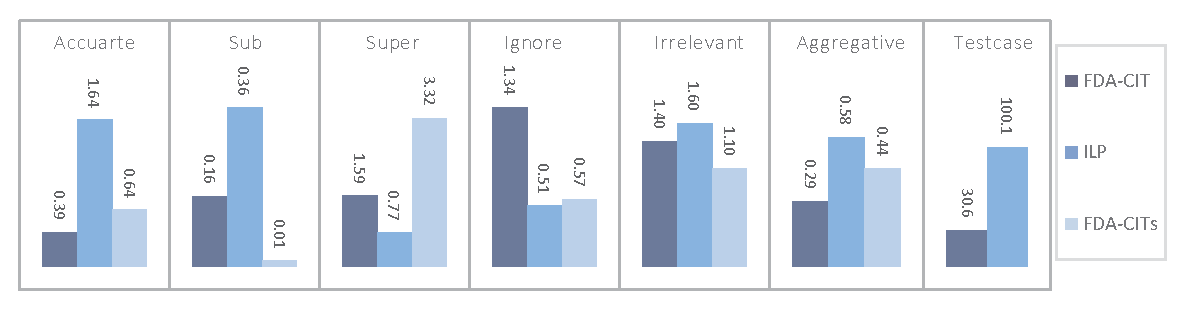
\includegraphics[width=5.4in]{2-way.eps}
}
\subfigure[Result for the 3-way covering array]{
  %  \rule{4cm}{3cm}
    \label{fig:32}
    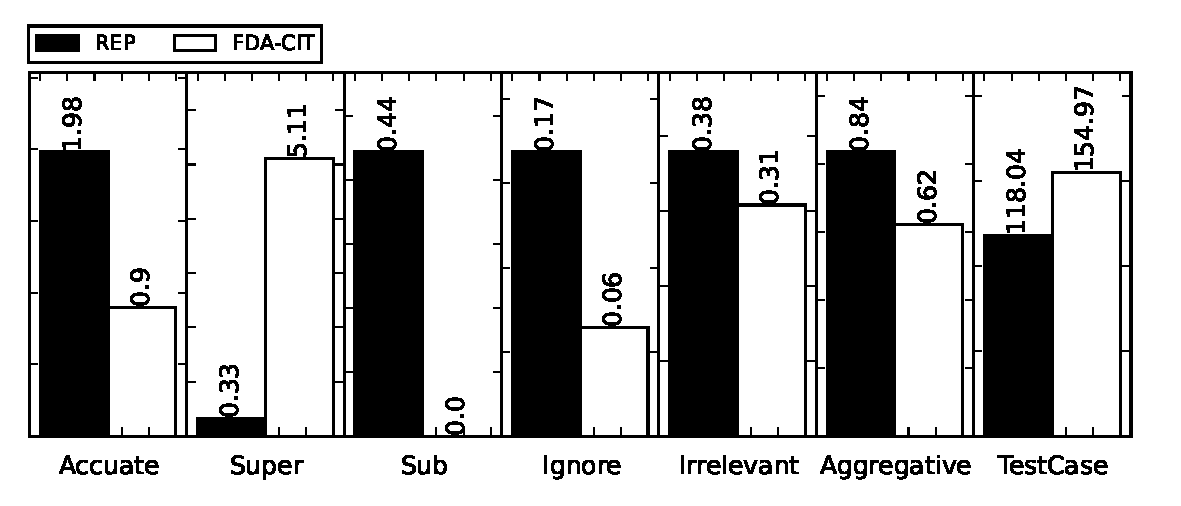
\includegraphics[width=5.4in]{3-way.eps}
}
\subfigure[Result of the 4-way covering array]{
  %  \rule{4cm}{3cm}
    \label{fig:33}
    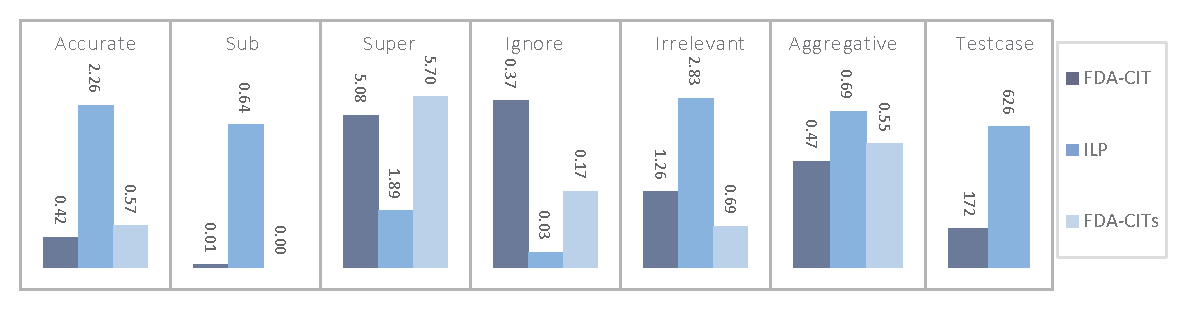
\includegraphics[width=5.4in]{4-way.eps}
}
\caption[Optional caption for list of figures]{Three approaches augmented with the replacing strategy}
\label{fig:comparefda}
\end{figure*}


With respect to the relationships between the results and the degree \emph{t} of the covering arrays, we have the following observations:

First, for every metric in our study, the order of the performance of each approach is stable against the change of degree \emph{t}. Take for example the metric \emph{accurate number}. No matter what \emph{t} is (2 , 3 or 4), \emph{ILP} always obtained the most schemas that are identical to the actual MFS, and then is \emph{FDA-CITs}, and the last is \emph{FDA-CIT}. This observation indicates that the difference between the performance of these approaches is not dependent on the characteristics of the covering array, but instead on the approaches themselves.

Second, with increasing \emph{t},  the overall performance of each approach is improved. For example, the score of the aggregative metric of \emph{ILP} is 0.55, 0.66 and 0.69, respectively, for \emph{t} equals to 2, 3 and 4. The improvement is mainly because with increasing \emph{t}, the number of test cases also increased. Based on this, the approach will observe more failing test cases (See area B in Figure \ref{fig:fci_process}), so that we can get the schemas more close to the actual MFS.

Third, for different approaches in our study, the effect of the change of \emph{t} on the scores of other metrics varies. Specifically, for \emph{ILP}, with increasing \emph{t}, metrics \emph{accurate number, sub number, super number, irrelevant number} also increase, while metric \emph{ignore number} decreases. This is mainly because \emph{ILP} is based on \emph{FIC\_BS} \cite{zhang2011characterizing}, which works on single failing test case. As we all know, when \emph{t} increases, the number of test cases also increases. Then when applying our approach, more different schemas may be identified from those additional failing test cases, so the number of accurate MFS, sub-schemas of the actual MFS, super-schemas of the actual MFS, and schemas that are irrelevant to the actual MFS will increase. Furthermore, some actual MFS that had been ignored before may be obtained.  For \emph{FDA-CIT} and \emph{FDA-CITs}, however, we find that \emph{sub number, irrelevant number} decrease with increasing \emph{t}.  We believe this result is due to the use of the classification tree method. A typical classification tree works by partitioning the test cases according to some aspects. Here, the aspect is the parameter value of the SUT. And one path (conjunction of nodes from the root to one leaf in the tree) in this tree is deemed as an MFS. So when test cases increase, the classification may need more nodes to classify the test cases. This induces the so-called `over fitting' problem. As a result, the schemas identified by \emph{FDA-CIT} and \emph{FDA-CITs} tend to be the super schemas of the actual MFS, leading to a decrease of \emph{sub number } and \emph{irrelevant number}.

Other observations include:

First, when compared with the original approach \emph{FDA-CIT}, \emph{FDA-CITs} has obvious advantages at almost all the metrics except for \emph{super number}. In detail, \emph{FDA-CITs} obtained more schemas that are identical to the actual MFS (\emph{accurate number}), less schemas that are the sub schemas of actual MFS (\emph{sub number}), and lower scores for the two negative metrics (\emph{ignored number} and \emph{irrelevant number}). At last, the schemas identified by \emph{FDA-CITs} showed an overall higher quality than that of the original \emph{FDA-CIT} (\emph{aggregative metric}).  We have discussed previously that \emph{FDA-CIT} tends to identify super-schemas of actual MFS when the test cases increase. So for metric \emph{super number}, it is no surprise that \emph{FDA-CITs} identified more super schemas of actual MFS than \emph{FDA-CIT}, because it used the test cases generated by \emph{ILP}, which were more than that of the original FDA-CIT. The difference between the overall performance of \emph{FDA-CIT} and \emph{FDA-CITs} is also expected. In fact, this result is consistent with our previous observation that when \emph{t} increases, the overall performance for each approach also increases.

%
%This result indicates that the number of test cases is a key factor that affects the performance of the approach FDA-CIT. And the more test cases are, the better the FDA-CIT will perform, though FDA-CIT would also identified more super schemas of the actual MFS.

Second, in terms of the quality of the MFS identified, we can clearly find that our approach performed better than the other approaches. This is mainly manifested in that our approach obtained more accurate schemas and identified less irrelevant ones. We believe this gap is mainly caused by the FCI approach. Because for \emph{ILP} and \emph{FDA-CITs}, the test cases used to identify the MFS are the same. The only difference is how they utilize them to identify MFS. However, this result does not mean that FIC\_BS is better than the classification tree method under all conditions. The classification tree method has its own advantage, i.e., it does not need to generate additional test cases, and as a result, \emph{FDA-CIT} generated less test cases than that of \emph{ILP}.

In fact, another reason why our approach generated more test cases is that the FCI approach, i.e., FIC\_BS , works on single test case, so when there are many failing test cases in the covering array, we need to repeatedly use our approach to identify the MFS for each failing test case. This process may produce many redundant test cases, because many failing test cases contain the same MFS, and when we have already identified the MFS in one test case, there is no need to identify it again in other failing test cases. Jieli \cite{li2012improved} introduced a method that utilizes the previous generated test cases to reduce such redundance. Here we did not use this technique to simplify our experiment. We believe if we utilize the MFS that are already identified in previous iteration, the overall number of test cases will decrease.

% The second reason that why our approach generated more test cases than \emph{FDA-CIT} is that .


%for the approaches \emph{FDA-CIT} and \emph{FDA-CITs}, we can find the latter performed better than the former.
%In terms of , we can have the following
%When we fix the degree \emph{t}, we can learn the following with respect to
%
%We firstly
%
%
%Then we .

Above all, we can conclude three points in this experiment, which provide answer to \textbf{Q4}:

%1) FDA serial ����, and the ILP ���ӿ��ţ���˸����ʺϡ�

1)The degree \emph{t} of the covering array does not determine the order of the performance of different approaches, but for each approach, the bigger the \emph{t} is, the better its performance will be.

2)When taking the test cases generated by our approach \emph{ILP}, \emph{FDA-CITs} performed better than the original \emph{FDA-CIT} approach.

3)Considering the quality of the MFS each approach identified, \emph{ILP} performed better than the other two approaches, although it needed more test cases.

Based on these observations, a recommendation for selecting masking handling techniques in practice is that to get a more precise identification of the  MFS in the SUT, \emph{ILP} is preferred, and for a small size of test cases,  \emph{FDA-CIT} may be a better choice.

%3)The increasing t a overall improvement for the quality but also increasing the test cases.

%
%From this result, we can first observe that in all the cases our ILP-based approach can more accurately identify the MFS and ignored less MFS than the FDA-CIT approach. For the metric `super-schema', `sub-schema', and `irrelevant schemas', there are ups and downs on both sides. With respect to the `overall metric', we find our approach has a significant advantage over the FDA-CIT, but it also requires many more test cases than FDA-CIT.
%
%We note that, when applying the multiple-class FCI to characterize the MFS with the test cases that were generated using our approach, their `overall' metric is still not as good as our ILP-based approach, but may show some improvement over the original FDA-CIT.
%
%Another interesting observation is that overall performance in most cases is increasing with the $t$, which can be easily understood. More test cases will contain more information about the MFS, so that we can utilize them to identify the MFS more precisely.
%
%%
%%the t more, the result is more good, but there must be the over-fit problem, for example, for.
%%
%%it is because the improvement by the t-coverage is increasing quickly when the bug is 2-4 or large than 2, if the bug itself is less than 2 -4 , than the improvement is not obviously.
%
%So the answer for \textbf{Q4} is that: our approach can achieved a more precise result for the MFS, and the FDA-CIT can perform the identifying process using a small amount extra test cases. Both of these two approaches have their ups and downs, choosing which approach in practice will depend on the specific scenario you test.
%% if you want to get a more precise result and more helpful test cases generating supply, you should choose our approach, however if you are limited to the test cases execution, you can choose the feedback driven.
%% but if
\subsection{Threats to validity}

%This section gives the threats to internal validity and external validity of our study.
%\subsubsection{construct threats}
%We use the five metrics to demonstrate the validate the effectiveness of our approach, this is derived from the intuitive point.

\subsubsection{internal threats}
There are two threats to internal validity. First, the characteristics of the actual MFS in the SUT can affect the FCI results.  This is because the magnitude and location of the MFS can make the FCI approaches generate different test cases. And as a result, it can make the observed failing test cases and predicted failing test cases different (See Figure \ref{fig:fci_process}). In the worst case, the FCI approach happens to identify the exact actual MFS, and in that condition our test case replacing strategy is of no use. In this paper, we used 15 testing objects, in which 5 are real software systems with real faults and 10 synthetic ones with injected faults. To reduce the influence caused by different characteristics of the MFS, we need to build more testing objects and injected more different types of faults for a more comprehensive study of our approach.

%
% The identifying approach can affect.
%
%The second threat comes from the input model we built. As we focused on the options related to the perfect combinations and only augmented it with some noise options, there is a chance we will get different results if we choose other noise options. More options needed to be tested to see whether our result is common or just appears in some particular input models.

The second threat is that we just applied our test case replacing strategy on one FCI approach -- FIC\_BS \cite{zhang2011characterizing}. Although we believe the test case replacing strategy can also improve the quality of the identified MFS for other FCI approaches when the testing object is suffering from masking effects, the extent to which their results can be refined may vary for different FCI approaches. For example, for FIC\_BS \cite{zhang2011characterizing} used in this paper, there are about $(v - 1)$ to $(v - 1)^{k - 1}$ candidate test cases that can be replaced (See Table \ref{fixed-part-complexisty}) when one test case triggered other failures, while for OFOT \cite{nie2011minimal}, we only have $(v - 1)$ candidates. As a result, FIC\_BS can have a higher chance than OFOT to find a satisfied test case.  So to learn the difference between the improvement of different FCI approaches when applying our test case replacing strategy, we need to try more FCI approaches in the future.

% And  so further works needed to examine more algorithms in this field to obtain a more general result.

\subsubsection{external threats}

One threat to external validity comes from the real software we used.  In this paper we have only surveyed two types of open-source software with five different versions, of which the program scale is medium-sized. This may impact the generality of our results.
% Although we believe it is quite possibly a common phenomenon in most software that contains multiple failures which can mask each other, we need to investigate more software to support our belief.


Another important threat is that our approach is based on the assumption that different errors in the software can be easily distinguished by information such as exception traces, state conditions, or the like. If we cannot directly distinguish them, our approach does not work. In such case, one potential solution is to use the clustering techniques to classify the failures according to available information \cite{zheng2006statistical,jones2007debugging,podgurski2003automated}. If we cannot classify them because we do not have enough information (e.g., the black box testing) or it is too costly, we believe the only approach is to take the \emph{regarded as one failure} strategy. With this strategy, we must aware that the MFS identified are likely to be sub-schemas or irrelevant schemas of the actual MFS.
%alleviate the impact of multiple faults is to take a trial-and-error process, i.e., initially classify failures by random and then identify the MFS and fix the bugs based on the classification, after which if the program still doesn't work, then the classification process will be refined and the previous steps continue.

The third threat comes from the possible masking relationships between multiple failures in the real software.  In this paper, we just focus on the condition that the masking effects are transitive, i.e., if failure \emph{A} masks \emph{B}, failure \emph{B} masks \emph{C}, then failure \emph{A} must mask the failure \emph{C}. In practice, the relationships between multiple failures may be more complicated. One possible scenario is that two failures are in a loop, for which the two failures can even mask each other in a particular condition. Such a case will make our formal analysis invalid and will significantly complicate the relationships between schemas and their corresponding test cases. A new formal model should be proposed to handle that type of masking effects.

%
% not the directly linear about multiple failures, i.e., failure a can mask the failure b, failure b can mask a . and failure c can mask failure c. Even worse, two failures can mask each other. When such scenorias happened, we need to recoonsruct the formal model of the schemas that when can be either be.  as the condition will significantly completed the relationships between the failures and schemas. But anyhow, our appraohc can still work in such a way, as the will always good to identify the MFS.

\section{related works}

Shi and Nie presented an approach for failure revealing and failure diagnosis in CT \cite{shi2005software}, which first tests the SUT with a covering array, then reduces the value schemas contained in the failing test case by eliminating those appearing in the passing test cases. If the failure-causing schema is found in the reduced schema set, failure diagnosis is completed with the identification of the specific input values which caused the failure; otherwise, a further test suite based on SOFOT is developed for each failing test cases, and the schema set is then further reduced, until no more faults are found or the fault is located. Based on this work, Wang proposed an AIFL approach which extended the SOFOT process by adaptively mutating factors in the original failing test cases in each iteration to characterize failure-inducing interactions \cite{wang2010adaptive}.

Nie et al. introduced the notion of Minimal Failure-causing Schema(MFS) and proposed the OFOT approach which is an extension of SOFOT that can isolate the MFS in SUT \cite{nie2011minimal}. This approach mutates one value with different values for that parameter, hence generating a group of additional test cases each time to be executed. Compared with SOFOT, this approach  strengthens the validation of the factor under analysis and can also detect the newly imported faulty interactions.

Delta debugging \cite{zeller2002simplifying} is an adaptive divide-and-conquer approach to locate interaction failure. It is very efficient and has been applied to real software environment. Zhang et al. also proposed a similar approach that can efficiently identify the failure-inducing interactions that has no overlapped part \cite{zhang2011characterizing}. Later, Li improved the delta-debugging based approach by exploiting useful information in the executed covering array \cite{li2012improved}.

Colbourn and McClary proposed a non-adaptive method \cite{colbourn2008locating}. Their approach extends a covering array to the locating array to detect and locate interaction failures. C. Martinez proposed two adaptive algorithms. The first one requires safe value as the assumption and the second one removes this assumption when the number of values of each parameter is equal to 2 \cite{martinez2008algorithms,martinez2009locating}. Their algorithms focus on identifying faulty tuples that have no more than 2 parameters.

Ghandehari et al. defined the suspiciousness of tuple and suspiciousness of the environment of a tuple \cite{ghandehari2012identifying}. Based on this, they ranked the possible tuples and generated the test configurations. They further utilized the test cases generated from the inducing interaction to locate the fault \cite{ghandehari2013fault}.

Yilmaz proposed a machine learning method to identify inducing interactions from a combinatorial testing set \cite{yilmaz2006covering}. They constructed a classification tree to analyze the covering arrays and detect potential faulty interactions. Beside this, Fouch{\'e} \cite{fouche2009incremental} and Shakya \cite{shakya2012isolating} made some improvements in identifying failure-inducing interactions based on Yilmaz's work.

Our previous work \cite{niu2013identifying} proposed an approach that utilizes the tuple relationship tree to isolate the failure-inducing interactions in a failing test case. One novelty of this approach is that it can identify the overlapped faulty interaction. This work also alleviates the problem of introducing new failure-inducing interactions in additional test cases.

In addition to the studies that aim at identifying the failure-inducing interactions in test cases, there are others that focus on working around the masking effects.

Constraints handling become more and more popular in CT these years. A constraint is an invalid interaction that should not appear in the test case. It can be deemed as the masking effect which are known in prior \cite{yilmaz2013reducing}.  Cohen \cite{cohen2007exploiting,cohen2007interaction,cohen2008constructing} studied the impact of the constraints that render some generated test cases invalid in CT. They also proposed an approach that integrates the incremental SAT solver with the covering arrays generating algorithm to avoid those invalid interactions. Further study was conducted \cite{petke2013efficiency} to show that with consideration of constrains, higher-strength covering arrays with early failure detection are practical.

Besides, there are additional works that aim to study the impacts of constraints for CT \cite{garvin2011evaluating,bryce2006prioritized,calvagna2008logic,grindal2006handling,yilmaz2013test}.
Among them, \cite{bryce2006prioritized} distinguished the constraints into two types: \emph{hard} and \emph{soft}, which the former cannot be included in the test case, while the latter can be permitted, but not desirable.  \cite{grindal2006handling} comprehensively compared the performance of four strategies at handling the constraints in the covering array. \cite{calvagna2008logic} proposed an heuristic strategy to handle the constraints. It can support an ad-hoc inclusion or exclusion of interactions such that the user can customize output of the covering array. \cite{garvin2011evaluating} refined the simulated annealing algorithm to efficiently construct the covering array with considering the constraints. \cite{yilmaz2013test} introduced the test case-specific constraints; differing from the system-wide constraints, this constraint can only be triggered in some specific test cases.
 %These approaches use some rules or to avoid these invalidated test cases to improve the efficiency when examine the test cases.

Chen et al. addressed the issues of shielding parameters in combinatorial testing and proposed the Mixed Covering Array with Shielding Parameters (MCAS) to solve the problem caused by shielding parameters \cite{chen2010combinatorial}. The shielding parameters can disable some parameter values to expose additional interaction errors, which can be regarded as a special case of masking effects.

Dumlu and Yilmaz proposed a feedback-driven approach to work around the masking effects \cite{dumlu2011feedback}. Specifically, they first used classification tree to classify the possible failure-inducing interactions and eliminate them. Then they generate new test cases to detect possible masked interaction in the next iteration. They further extended their work \cite{yilmaz2013reducing} by proposing a multiple-class CTA approach to distinguish failures in SUT. In addition, they empirically studied the impacts of masking effects on both ternary-class and multiple-class CTA approaches.


These works can be categorized into 3 groups according to their relationships with our work. First, the works that aim to identifying the MFS in the SUT. Our work also focuses on identifying the MFS, but instead of single failure, our work considers the impacts of multiple failures on the FCI approaches, and based on this, a test case replacement strategy is proposed that can assist these FCI approaches in reducing the negative effects. Second, the works that aim to handling the constraints. As discussed before the constraints can be deemed as a special masking effects. Our work differs from them in that the masking effects handled in this paper are those that can be dynamically triggered; that is, we did not know them in prior. Another difference between our work with these constraints handling works is that their target is to avoid the constraints when generating covering array. However, our work aims to removing the masking effects of the FCI approaches.  Last, the work that is most similar to our work \cite{yilmaz2013reducing}, which also considered the masking effects that are dynamically appeared in test cases. But different from our work, it mainly focused on reducing the masking effects in the covering array, so that the covering array can support a comprehensive validation of all the t-degree schemas. The approach used to reduce this negative effect is to use the FCI approach to identify the schemas that can trigger this effect in each iteration. Our approach, however, aims to handling the masking effects that happened in these FCI approaches themselves, and our approach alleviates the masking effects by augmenting the FCI approaches with a test case replacement strategy.
%\cite{shi2005software,wang2010adaptive,nie2011minimal,zhang2011characterizing,li2012improved,colbourn2008locating,martinez2008algorithms ,martinez2009locating,yilmaz2006covering,shakya2012isolating,ghandehari2012identifying,niu2013identifying}
%Our work differs from these mainly in that we formally studied the masking effects on FCI approaches and further proposed a divide-and-conquer strategy to alleviate this impact.

\section{Conclusions}
Masking effects of multiple failures in SUT can bias the results of traditional failure-inducing interactions identifying approaches. In this paper, we formally analysed the impact of masking effects on FCI approaches and showed that the two traditional strategies, i.e., \emph{regarded as one fault} and \emph{distinguishing failures}, are both inefficient in handling such impact. We further presented a test case replacement strategy for FCI approaches to alleviate such impact.

%This strategy separately handle each failure in SUT, and for a particular failure, it will discard these test cases that trigger failures different from the one under analysis and only keep those that either pass or trigger the expected failure. Additional test cases for compensation will be generated after discarding unsatisfied test cases.

In our empirical studies, we extended FIC\_BS \cite{zhang2011characterizing} with our strategy. The comparison between our approach and traditional approaches was performed on several open-source software. The results indicated our strategy assists the traditional FCI approach in achieving better performance when facing masking effects in SUT. We also empirically evaluated the efficiency of the test case searching component by comparing it with the random searching based FCI approach. The results showed that the ILP-based test case searching method can perform more efficiently. Last, we compared our approach with existing technique for handling masking effects -- FDA-CIT \cite{yilmaz2013reducing}, and observed that our approach achieved a more precise result which can better support  debugging, though our approach required more test cases than FDA-CIT.

As for the future work, we need to do more empirical studies to make our conclusions more general. Our current experiments focus on medium-sized software. We would like to extend our approach to more complicated, large-scaled testing scenarios. Another promising work in the future is to integrate the white-box testing technique into the FCI approaches. We believe gaining insight into source code can help figure out the relationships between multiple failures, and hence facilitate the FCI approaches obtaining more accurate results. And last, because the extent to which the FCI suffers from masking effects varies with different algorithms, combining these different FCI approaches would be desired in the future to further improve identifying MFS for multiple failures.



% Start of "Sample References" section

%\section{Typical references in new ACM Reference Format}
%%A paginated journal article \cite{Abril07}, an enumerated
%%journal article \cite{Cohen07}, a reference to an entire issue \cite{JCohen96},
%%a monograph (whole book) \cite{Kosiur01}, a monograph/whole book in a series (see 2a in spec. document)
%%\cite{Harel79}, a divisible-book such as an anthology or compilation \cite{Editor00}
%%followed by the same example, however we only output the series if the volume number is given
%%\cite{Editor00a} (so Editor00a's series should NOT be present since it has no vol. no.),
%%a chapter in a divisible book \cite{Spector90}, a chapter in a divisible book
%%in a series \cite{Douglass98}, a multi-volume work as book \cite{Knuth97},
%%an article in a proceedings (of a conference, symposium, workshop for example)
%%(paginated proceedings article) \cite{Andler79}, a proceedings article
%%with all possible elements \cite{Smith10}, an example of an enumerated
%%proceedings article \cite{VanGundy07},
%%an informally published work \cite{Harel78}, a doctoral dissertation \cite{Clarkson85},
%%a master's thesis: \cite{anisi03}, an online document / world wide web resource \cite{Thornburg01}, \cite{Ablamowicz07},
%%\cite{Poker06}, a video game (Case 1) \cite{Obama08} and (Case 2) \cite{Novak03}
%%and \cite{Lee05} and (Case 3) a patent \cite{JoeScientist001},
%%work accepted for publication \cite{rous08}, 'YYYYb'-test for prolific author
%%\cite{SaeediMEJ10} and \cite{SaeediJETC10}. Other cites might contain
%%'duplicate' DOI and URLs (some SIAM articles) \cite{Kirschmer:2010:AEI:1958016.1958018}.
%%Boris / Barbara Beeton: multi-volume works as books
%%\cite{MR781536} and \cite{MR781537}.
%
%% Appendix
%\appendix
%\section*{APPENDIX}
%\setcounter{section}{1}
%
%
%\appendixhead{ZHOU}

% Acknowledgments
%\begin{acks}
%The authors would like to thank Dr. Maura Turolla of Telecom
%Italia for providing specifications about the application scenario.
%\end{acks}

% Bibliography
\bibliographystyle{ACM-Reference-Format-Journals}
\bibliography{acmsmall-sample-bibfile}
                             % Sample .bib file with references that match those in
                             % the 'Specifications Document (V1.5)' as well containing
                             % 'legacy' bibs and bibs with 'alternate codings'.
                             % Gerry Murray - March 2012

% History dates
%\received{February 2007}{March 2009}{June 2009}

% Electronic Appendix
\elecappendix

\medskip

\section{Detail Propositions for masking effects}
\begin{itemize}
\item $T_{as} = B_{1} \bigcup B_{2} \bigcup C \bigcup D$ indicates all the actual failing test cases.
\item $T_{km} = A \bigcup B_{1} \bigcup B_{2} \bigcup C$  indicates the test cases for strategy \emph{knowing masking effects}.
\item $T_{ro} = A \bigcup B_{1} \bigcup B_{2} \bigcup B_{3} \bigcup C $ indicates the test cases for strategy \emph{regarded as one failure}
\item $T_{df} = A \bigcup B_{1} \bigcup C$  indicates the test cases for strategy \emph{distinguishing failures}
\end{itemize}

\subsection{For \emph{regarded as one failure} in Table \ref{conditions-for-ro}}

\begin{proposition}[rule 1]\label{pro:appendix1rule1}
$\forall c_{ro} \in \mathcal{C}(T_{ro})$ if $\exists c_{km} \in \mathcal{C}(T_{km}),\ s.t.,\ c_{ro} = c_{km}$, and correspondingly, $\exists c_{as} \in \mathcal{C}(T_{as}),\ s.t.,\ c_{km} = c_{as}$. Then it must have $c_{ro} = c_{as}$.
\end{proposition}
%\begin{proof}
%\end{proof}
\begin{proposition}[rule 2]\label{pro:appendix1rule2}
$\forall c_{ro} \in \mathcal{C}(T_{ro})$ if $\exists c_{km} \in \mathcal{C}(T_{km}),\ s.t.,\ c_{ro} = c_{km}$, and correspondingly, $\exists c_{as} \in \mathcal{C}(T_{as}),\ s.t.,\ c_{as} \prec c_{km}$. Then it must have $c_{as} \prec c_{ro}$.
\end{proposition}

\begin{proposition}[rule 3]\label{pro:appendix1rule3}
$\forall c_{ro} \in \mathcal{C}(T_{ro})$ if $\exists c_{km} \in \mathcal{C}(T_{km}),\ s.t.,\ c_{ro} = c_{km}$, and correspondingly, $\exists c_{as} \in \mathcal{C}(T_{as}),\ s.t.,\ c_{km} \prec c_{as}$. Then it must have $c_{ro} \prec c_{as}$.
\end{proposition}

\begin{proposition}[rule 4]\label{pro:appendix1rule4}
$\forall c_{ro} \in \mathcal{C}(T_{ro})$ if $\exists c_{km} \in \mathcal{C}(T_{km}),\ s.t.,\ c_{ro} = c_{km}$, and correspondingly, $c_{km}\ is\ irrelevant\ to\  \mathcal{C}(T_{as})$. Then it must have $c_{ro} \ is\ irrelevant\ to\  \mathcal{C}(T_{as})$.
\end{proposition}

\begin{proposition}[rule 5]\label{pro:appendix1rule5}
$\forall c_{ro} \in \mathcal{C}(T_{ro})$ if $\exists c_{km} \in \mathcal{C}(T_{km}),\ s.t.,\ c_{ro} \prec c_{km}$, and correspondingly, $\exists c_{as} \in \mathcal{C}(T_{as}),\ s.t.,\ c_{km} = c_{as}$. Then it must have $c_{ro} \prec c_{as}$.
\end{proposition}

\begin{proposition}[rule 6]\label{pro:appendix1rule6}
$\forall c_{ro} \in \mathcal{C}(T_{ro})$ if $\exists c_{km} \in \mathcal{C}(T_{km}),\ s.t.,\ c_{ro} \prec c_{km}$, and correspondingly, $\exists c_{as} \in \mathcal{C}(T_{as}),\ s.t.,\ c_{as} \prec c_{km}$. Then it must have $\exists c_{as}' \in \mathcal{C}(T_{as}),\ s.t.,\ c_{ro} \prec c_{as}'\ or\ c_{ro}\ irrelevant\ to\ \mathcal{C}(T_{as})$.
\end{proposition}
\begin{proof}


\end{proof}


\begin{proposition}[rule 7]\label{pro:appendix1rule7}
$\forall c_{ro} \in \mathcal{C}(T_{ro})$ if $\exists c_{km} \in \mathcal{C}(T_{km}),\ s.t.,\ c_{ro} \prec c_{km}$, and correspondingly, $\exists c_{as} \in \mathcal{C}(T_{as}),\ s.t.,\ c_{km} \prec c_{as}$. Then it must have $c_{ro} \prec c_{as}$.
\end{proposition}

\begin{proposition}[rule 8]\label{pro:appendix1rule8}
$\forall c_{ro} \in \mathcal{C}(T_{ro})$ if $\exists c_{km} \in \mathcal{C}(T_{km}),\ s.t.,\ c_{ro} = c_{km}$, and correspondingly, $c_{km}\ is\ irrelevant\ to\  \mathcal{C}(T_{as})$. Then it must have $\exists c_{as}  \in \mathcal{C}(T_{as}),\ s.t.,\ c_{ro} \prec c_{as}\ or\ c_{ro}\ irrelevant\ to\ \mathcal{C}(T_{as})$.
\end{proposition}
\begin{proof}


\end{proof}

\begin{proposition}[rule 9]\label{pro:appendix1rule9}
$\forall c_{ro} \in \mathcal{C}(T_{ro})$ if $c_{ro} \ is\ irrelevant\ to\  \mathcal{C}(T_{km})$. Then it must have $\exists c_{as}  \in \mathcal{C}(T_{as}),\ s.t.,\ c_{ro} \prec c_{as}\ or\ c_{ro}\ is\ irrelevant\ to\ \mathcal{C}(T_{as})$.
\end{proposition}
\begin{proof}


\end{proof}

\subsection{For \emph{regarded as one failure} in Table \ref{conditions-for-ro-ignore}}


\begin{proposition}[rule 1]\label{pro:appendix1rule1i}
$\forall c_{as} \in \mathcal{C}(T_{as})$ if $\exists c_{km} \in \mathcal{C}(T_{km}),\ s.t.,\ c_{as} = c_{km}$, and correspondingly, $\exists c_{ro} \in \mathcal{C}(T_{ro}),\ s.t.,\ c_{km} = c_{ro}$. Then it must have $c_{ro} = c_{as}$.
\end{proposition}

\begin{proposition}[rule 2]\label{pro:appendix1rule2i}
$\forall c_{as} \in \mathcal{C}(T_{as})$ if $\exists c_{km} \in \mathcal{C}(T_{km}),\ s.t.,\ c_{as} = c_{km}$, and correspondingly, $\exists c_{ro} \in \mathcal{C}(T_{ro}),\ s.t.,\ c_{ro} \prec c_{km}$. Then it must have $c_{ro} \prec c_{as}$.
\end{proposition}

\begin{proposition}[rule 3]\label{pro:appendix1rule3i}
$\forall c_{as} \in \mathcal{C}(T_{as})$ if $\exists c_{km} \in \mathcal{C}(T_{km}),\ s.t.,\ c_{as} \prec c_{km}$, and correspondingly, $\exists c_{ro} \in \mathcal{C}(T_{ro}),\ s.t.,\ c_{km} = c_{ro}$. Then it must have $c_{as} \prec c_{ro}$.
\end{proposition}

\begin{proposition}[rule 4]\label{pro:appendix1rule4i}
$\forall c_{as} \in \mathcal{C}(T_{as})$ if $\exists c_{km} \in \mathcal{C}(T_{km}),\ s.t.,\ c_{as} \prec c_{km}$, and correspondingly, $\exists c_{ro} \in \mathcal{C}(T_{ro}),\ s.t.,\ c_{ro} \prec c_{km}$. Then it must have $c_{as} \ is\ irrelevant\ to\ \mathcal{C}(T_{ro})\ or\  \exists c_{ro}' \in \mathcal{C}(T_{ro}),\ s.t.,\ c_{as} \prec c_{ro}'$.
\end{proposition}
\begin{proof}


\end{proof}

\begin{proposition}[rule 5]\label{pro:appendix1rule5i}
$\forall c_{as} \in \mathcal{C}(T_{as})$ if $\exists c_{km} \in \mathcal{C}(T_{km}),\ s.t.,\ c_{km} \prec c_{as}$, and correspondingly, $\exists c_{ro} \in \mathcal{C}(T_{ro}),\ s.t.,\ c_{km} = c_{ro}$. Then it must have $c_{ro} \prec c_{as}$.
\end{proposition}

\begin{proposition}[rule 6]\label{pro:appendix1rule6i}
$\forall c_{as} \in \mathcal{C}(T_{as})$ if $\exists c_{km} \in \mathcal{C}(T_{km}),\ s.t.,\ c_{km} \prec c_{as}$, and correspondingly, $\exists c_{ro} \in \mathcal{C}(T_{ro}),\ s.t.,\ c_{ro} \prec c_{km}$. Then it must have $c_{ro} \prec c_{as}$.
\end{proposition}

\begin{proposition}[rule 7]\label{pro:appendix1rule7i}
$\forall c_{as} \in \mathcal{C}(T_{as})$ if $c_{as}\ is\ irrelevant\ to\ \mathcal{C}(T_{km}) $. Then it must have $c_{as} \ is\ irrelevant\ to\ \mathcal{C}(T_{ro})$.
\end{proposition}
\begin{proof}

\end{proof}


\subsection{For \emph{distinguishing failures} in Table \ref{conditions-for-df}}

\begin{proposition}[rule 1]\label{pro:appendix2rule1}
$\forall c_{df} \in \mathcal{C}(T_{df})$ if $\exists c_{km} \in \mathcal{C}(T_{km}),\ s.t.,\ c_{df} = c_{km}$, and correspondingly, $\exists c_{as} \in \mathcal{C}(T_{as}),\ s.t.,\ c_{km} = c_{as}$. Then it must have $c_{df} = c_{as}$.
\end{proposition}
%\begin{proof}
%\end{proof}
\begin{proposition}[rule 2]\label{pro:appendix2rule2}
$\forall c_{df} \in \mathcal{C}(T_{df})$ if $\exists c_{km} \in \mathcal{C}(T_{km}),\ s.t.,\ c_{df} = c_{km}$, and correspondingly, $\exists c_{as} \in \mathcal{C}(T_{as}),\ s.t.,\ c_{as} \prec c_{km}$. Then it must have $c_{as} \prec c_{df}$.
\end{proposition}

\begin{proposition}[rule 3]\label{pro:appendix2rule3}
$\forall c_{df} \in \mathcal{C}(T_{df})$ if $\exists c_{km} \in \mathcal{C}(T_{km}),\ s.t.,\ c_{df} = c_{km}$, and correspondingly, $\exists c_{as} \in \mathcal{C}(T_{as}),\ s.t.,\ c_{km} \prec c_{as}$. Then it must have $c_{df} \prec c_{as}$.
\end{proposition}

\begin{proposition}[rule 4]\label{pro:appendix2rule4}
$\forall c_{df} \in \mathcal{C}(T_{df})$ if $\exists c_{km} \in \mathcal{C}(T_{km}),\ s.t.,\ c_{df} = c_{km}$, and correspondingly, $c_{km}\ is\ irrelevant\ to\  \mathcal{C}(T_{as})$. Then it must have $c_{df} \ is\ irrelevant\ to\  \mathcal{C}(T_{as})$.
\end{proposition}

\begin{proposition}[rule 5]\label{pro:appendix2rule5}
$\forall c_{df} \in \mathcal{C}(T_{df})$ if $\exists c_{km} \in \mathcal{C}(T_{km}),\ s.t.,\ c_{km} \prec c_{df}$, and correspondingly, $\exists c_{as} \in \mathcal{C}(T_{as}),\ s.t.,\ c_{km} = c_{as}$. Then it must have $c_{as} \prec c_{df}$.
\end{proposition}

\begin{proposition}[rule 6]\label{pro:appendix2rule6}
$\forall c_{df} \in \mathcal{C}(T_{df})$ if $\exists c_{km} \in \mathcal{C}(T_{km}),\ s.t.,\ c_{km} \prec c_{df}$, and correspondingly, $\exists c_{as} \in \mathcal{C}(T_{as}),\ s.t.,\ c_{as} \prec c_{km}$. Then it must have $c_{as} \prec c_{df}$.
\end{proposition}

\begin{proposition}[rule 7]\label{pro:appendix2rule7}
$\forall c_{df} \in \mathcal{C}(T_{df})$ if $\exists c_{km} \in \mathcal{C}(T_{km}),\ s.t.,\ c_{km} \prec c_{df}$, and correspondingly, $\exists c_{as} \in \mathcal{C}(T_{as}),\ s.t.,\ c_{km} \prec c_{as}$. Then it must have $\exists c_{as}' \in \mathcal{C}(T_{as}),\ s.t.,\ c_{df} = c_{as}'\ or\ c_{as}' \prec c_{df}\ or\ c_{df} \prec c_{as}'\ or\ c_{df}\ irrelevant\ to\ \mathcal{C}(T_{as})$.
\end{proposition}

\begin{proof}


\end{proof}

\begin{proposition}[rule 8]\label{pro:appendix2rule8}
$\forall c_{df} \in \mathcal{C}(T_{df})$ if $\exists c_{km} \in \mathcal{C}(T_{km}),\ s.t.,\ c_{km} \prec c_{df}$, and correspondingly, $c_{km}\ is\ irrelevant\ to\  \mathcal{C}(T_{as})$. Then it must have $\exists c_{as}  \in \mathcal{C}(T_{as}),\ s.t.,\ c_{as} \prec c_{df}\ or\ c_{df}\ irrelevant\ to\ \mathcal{C}(T_{as})$.
\end{proposition}
\begin{proof}


\end{proof}

\subsection{For \emph{distinguishing failures} in Table \ref{conditions-for-df-ignore}}
\begin{proposition}[rule 1]\label{pro:appendix2rule1i}
$\forall c_{as} \in \mathcal{C}(T_{as})$ if $\exists c_{km} \in \mathcal{C}(T_{km}),\ s.t.,\ c_{as} = c_{km}$, and correspondingly, $\exists c_{df} \in \mathcal{C}(T_{df}),\ s.t.,\ c_{km} = c_{df}$. Then it must have $c_{df} = c_{as}$.
\end{proposition}

\begin{proposition}[rule 2]\label{pro:appendix2rule2i}
$\forall c_{as} \in \mathcal{C}(T_{as})$ if $\exists c_{km} \in \mathcal{C}(T_{km}),\ s.t.,\ c_{as} = c_{km}$, and correspondingly, $\exists c_{df} \in \mathcal{C}(T_{df}),\ s.t.,\ c_{km} \prec c_{df}$. Then it must have $c_{as} \prec c_{df}$.
\end{proposition}

\begin{proposition}[rule 3]\label{pro:appendix2rule3i}
$\forall c_{as} \in \mathcal{C}(T_{as})$ if $\exists c_{km} \in \mathcal{C}(T_{km}),\ s.t.,\ c_{as} = c_{km}$, and correspondingly, $c_{km} \ is\ irrelevant\ to\ \mathcal{C}(T_{df})$. Then it must have $c_{as} \ is\ irrelevant\ to\ \mathcal{C}(T_{df})$.
\end{proposition}

\begin{proposition}[rule 4]\label{pro:appendix2rule4i}
$\forall c_{as} \in \mathcal{C}(T_{as})$ if $\exists c_{km} \in \mathcal{C}(T_{km}),\ s.t.,\ c_{as} \prec c_{km}$, and correspondingly, $\exists c_{df} \in \mathcal{C}(T_{df}),\ s.t.,\ c_{df} = c_{km}$. Then it must have $c_{as} \prec c_{df}$.
\end{proposition}

\begin{proposition}[rule 5]\label{pro:appendix2rule5i}
$\forall c_{as} \in \mathcal{C}(T_{as})$ if $\exists c_{km} \in \mathcal{C}(T_{km}),\ s.t.,\ c_{as} \prec c_{km}$, and correspondingly, $\exists c_{df} \in \mathcal{C}(T_{df}),\ s.t.,\ c_{km} \prec c_{df}$. Then it must have $c_{as} \prec c_{df}$.
\end{proposition}


\begin{proposition}[rule 6]\label{pro:appendix2rule6i}
$\forall c_{as} \in \mathcal{C}(T_{as})$ if $\exists c_{km} \in \mathcal{C}(T_{km}),\ s.t.,\ c_{as} \prec c_{km}$, and correspondingly, $c_{km} \ is\ irrelevant\ to\ \mathcal{C}(T_{df})$. Then it must have $c_{as} \ is\ irrelevant\ to\ \mathcal{C}(T_{df})\ or\ \exists c_{df} \in s.t.,\ c_{as} \prec c_{df}$.
\end{proposition}
\begin{proof}
two contradtion

\end{proof}

\begin{proposition}[rule 7]\label{pro:appendix2rule7i}
$\forall c_{as} \in \mathcal{C}(T_{as})$ if $\exists c_{km} \in \mathcal{C}(T_{km}),\ s.t.,\ c_{km} \prec c_{as}$, and correspondingly, $\exists c_{df} \in \mathcal{C}(T_{df}),\ s.t.,\ c_{km} = c_{df}$. Then it must have $c_{df} \prec c_{as}$.
\end{proposition}

\begin{proposition}[rule 8]\label{pro:appendix2rule8i}
$\forall c_{as} \in \mathcal{C}(T_{as})$ if $\exists c_{km} \in \mathcal{C}(T_{km}),\ s.t.,\ c_{km} \prec c_{as}$, and correspondingly, $\exists c_{df} \in \mathcal{C}(T_{df}),\ s.t.,\ c_{km} \prec c_{df}$. Then it must have $\exists c_{df}' \in \mathcal{C}(T_{df}),\ s.t.,\ c_{as} = c_{df}'\ or\ c_{df}' \prec c_{as}\ or\ c_{as} \prec c_{df}'\ or\ c_{as}\ irrelevant\ to\ \mathcal{C}(T_{df})$.
\end{proposition}

\begin{proof}

\end{proof}

\begin{proposition}[rule 9]\label{pro:appendix2rule9i}
$\forall c_{as} \in \mathcal{C}(T_{as})$ if $\exists c_{km} \in \mathcal{C}(T_{km}),\ s.t.,\ c_{km} \prec c_{km}$, and correspondingly, $c_{km}\ is\ irrelevant\ to\  \mathcal{C}(T_{df})$. Then it must have $c_{as}\ irrelevant\ \mathcal{C}(T_{df})\ or\ \exists c_{df} \in \mathcal{C}(T_{df})\ s.t.,\ c_{df} \prec c_{as}$.
\end{proposition}
\begin{proof}
Assume $\exists c_{df} = c_{as}$, then $c_{km} \prec c_{df}$, contradiction. Assume $\exists c_{as} \prec c_{df}$, then $c_{km} \prec c_{df}$. Contradiction.

So it is only possible $c_{as}\ irrelevant\ \mathcal{C}(T_{df})\ or\ \exists c_{df} \in \mathcal{C}(T_{df})\ s.t.,\ c_{df} \prec c_{as}$. (One for example, One for example).
\end{proof}

\begin{proposition}[rule 10]\label{pro:appendix2rule10i}
$\forall c_{as} \in \mathcal{C}(T_{as})$ if $c_{as}\ is\ irrelevant\ to\ \mathcal{C}(T_{km}) $. Then it must have $c_{as} \ is\ irrelevant\ to\ \mathcal{C}(T_{df})$.
\end{proposition}


\section{The detail of the experiments}


\begin{table}[htbp]
\begin{threeparttable}
\tbl{Result of the evaluation of each appraoch\label{evaluation_all}}{
\setlength\tabcolsep{2pt}
 \begin{tabular}{|l|llll|llll|llll|llll|llll|llll|llll}
\hline
\textbf{Subject} & \multicolumn{4}{l|}{\textbf{accurate}} & \multicolumn{4}{l|}{\textbf{sub}} & \multicolumn{4}{l|}{\textbf{super}} & \multicolumn{4}{l|}{\textbf{ignore}}  & \multicolumn{4}{l|}{\textbf{irrelevant}} & \multicolumn{4}{l|}{\textbf{overall}} & \multicolumn{4}{l|}{\textbf{test cases}}           \\ \hline
                 & O \tnote{1}        & D  \tnote{2}      & I   \tnote{3}     & R  \tnote{4}      & O       & D      & I      & R     & O       & D        & I      & R      & O       & D       & I       & R       & O        & D        & I        & R       & O       & D       & I       & R       & O     & D     & I     & \multicolumn{1}{l|}{R}     \\
HSQLDB 2cr8      & 2        & 3       & 5       & 5       & 3       & 2      & 0      & 2     & 0       & 2        & 4      & 5      & 0(2.04) & 0(3.91) & 0(4.0)  & 0(4.1)  & 0        & 2        & 0        & 34      & 0.57    & 0.65    & 0.88    & 0.23    & 8.125 & 11.92 & 17    & \multicolumn{1}{l|}{17.72} \\
HSQLDB 2.2.5     & 2        & 2       & 2       & 2       & 1       & 0      & 0      & 0     & 0       & 1        & 1      & 1      & 0(0.83) & 0(1.0)  & 0(1.0)  & 0(1.0)  & 7        & 0        & 0        & 0       & 0.25    & 0.83    & 0.83    & 0.83    & 8.67  & 7.67  & 10.17 & \multicolumn{1}{l|}{11.3}  \\
HSQLDB 2.2.9     & 2        & 3       & 2       & 2       & 3       & 1      & 1      & 1     & 0       & 4        & 1      & 1      & 0(1.33) & 0(2.83) & 0(2.56) & 0(2.56) & 4        & 0        & 0        & 0       & 0.4     & 0.74    & 0.8     & 0.8     & 9.167 & 8.61  & 11.72 & \multicolumn{1}{l|}{13.14} \\
JFlex 1.4.1      & 2        & 2       & 2       & 2       & 0       & 0      & 0      & 0     & 0       & 1        & 0      & 0      & 0(0.75) & 0(1.0)  & 0(1.0)  & 0(1.0)  & 25       & 0        & 0        & 0       & 0.07    & 0.83    & 1       & 1       & 23.5  & 6.5   & 8     & \multicolumn{1}{l|}{9.68}  \\
JFlex 1.4.2      & 2        & 2       & 2       & 2       & 1       & 0      & 0      & 0     & 0       & 1        & 1      & 1      & 0(0.67) & 0(1.0)  & 0(1.0)  & 0(1.0)  & 25       & 0        & 0        & 0       & 0.09    & 0.83    & 0.83    & 0.83    & 20.5  & 9     & 11.67 & \multicolumn{1}{l|}{13.12} \\
synthez 1        & 2        & 1       & 1       & 1       & 2       & 0      & 0      & 0     & 0       & 2        & 2      & 2      & 0(1.0)  & 0(2.0)  & 0(2.0)  & 0(2.0)  & 15       & 17       & 17       & 17      & 0.19    & 0.11    & 0.11    & 0.11    & 16.5  & 18    & 41.75 & \multicolumn{1}{l|}{41.75} \\
synthez 2        & 3        & 3       & 3       & 3       & 10      & 0      & 0      & 0     & 0       & 10       & 6      & 6      & 0(1.96) & 0(2.0)  & 0(2.0)  & 0(2.0)  & 1        & 0        & 0        & 0       & 0.54    & 0.76    & 0.8     & 0.8     & 11.19 & 14.12 & 16.96 & \multicolumn{1}{l|}{17.08} \\
synthez 3        & 4        & 3       & 3       & 3       & 4       & 2      & 2      & 2     & 0       & 5        & 5      & 5      & 0(2.08) & 0(2.84) & 0(2.84) & 0(2.84) & 13       & 9        & 9        & 9       & 0.28    & 0.34    & 0.34    & 0.34    & 12.73 & 9.46  & 14.18 & \multicolumn{1}{l|}{14.44} \\
synthez 4        & 3        & 3       & 3       & 3       & 10      & 3      & 2      & 3     & 0       & 6        & 5      & 5      & 0(2.6)  & 0(2.8)  & 0(2.9)  & 0(2.85) & 9        & 9        & 9        & 9       & 0.35    & 0.4     & 0.39    & 0.39    & 9.91  & 13.02 & 18.55 & \multicolumn{1}{l|}{18.45} \\
synthez 5        & 2        & 2       & 2       & 2       & 4       & 0      & 0      & 0     & 0       & 2        & 1      & 1      & 0(1.02) & 0(1.0)  & 0(1.0)  & 0(1.0)  & 1        & 0        & 0        & 0       & 0.65    & 0.88    & 0.92    & 0.92    & 13.04 & 13.7  & 14.77 & \multicolumn{1}{l|}{14.84} \\
synthez 6        & 2        & 3       & 3       & 3       & 15      & 4      & 4      & 4     & 0       & 8        & 8      & 8      & 0(1.99) & 0(3.72) & 0(3.72) & 0(3.72) & 8        & 10       & 10       & 10      & 0.38    & 0.36    & 0.36    & 0.36    & 14.91 & 11.75 & 15.37 & \multicolumn{1}{l|}{15.71} \\
synthez 7        & 3        & 3       & 3       & 3       & 10      & 0      & 0      & 0     & 0       & 6        & 6      & 6      & 0(2.04) & 0(2.0)  & 0(2.0)  & 0(2.0)  & 5        & 0        & 0        & 0       & 0.39    & 0.83    & 0.83    & 0.83    & 12.77 & 14.59 & 16.44 & \multicolumn{1}{l|}{16.53} \\
synthez 8        & 2        & 2       & 2       & 2       & 4       & 0      & 0      & 9     & 0       & 4        & 3      & 3      & 0(1.05) & 0(1.0)  & 0(1.0)  & 0(1.0)  & 3        & 0        & 0        & 0       & 0.56    & 0.9     & 0.91    & 0.91    & 24.45 & 25.25 & 26.27 & \multicolumn{1}{l|}{26.37} \\
synthez 9        & 2        & 1       & 1       & 1       & 1       & 0      & 0      & 0     & 0       & 1        & 1      & 1      & 0(0.8)  & 0(1.0)  & 0(1.0)  & 0(1.0)  & 0        & 0        & 0        & 0       & 0.75    & 0.83    & 0.83    & 0.83    & 6.8   & 8     & 9     & \multicolumn{1}{l|}{9}     \\
synthez 10       & 0        & 1       & 1       & 1       & 3       & 1      & 1      & 1     & 0       & 0        & 0      & 0      & 0(1.0)  & 0(1.46) & 0(1.31) & 0(1.31) & 0        & 2        & 1        & 1       & 0.5     & 0.47    & 0.58    & 0.58    & 9.08  & 11    & 15.38 & \multicolumn{1}{l|}{15.53} \\ \hline
\end{tabular}
    }

     \begin{tablenotes}
        \footnotesize
        \item[1] $O$ denotes the strategy \emph{regarded as one failure}.
        \item[2] $D$ denotes the strategy \emph{distinguishing failures}.
        \item[3] $I$ denotes the replacement strategy based on ILP searching.
        \item[4] $R$ denotes the replacement strategy based on randomly searching.
      \end{tablenotes}
%  \label{tab:addlabel}%
\end{threeparttable}
\end{table}%

\begin{table}[htbp]
\begin{threeparttable}
\tbl{Comparison with FDA-CIT\label{comparewithfda}}{
\setlength{\tabcolsep}{3pt}
\begin{tabular}{|l|l|lll|lll|lll|lll|lll|lll|lll}
\hline
\textbf{Subject} & \textbf{} & \multicolumn{3}{l|}{\textbf{accurate}} & \multicolumn{3}{l|}{\textbf{sub}} & \multicolumn{3}{l|}{\textbf{super}} & \multicolumn{3}{l|}{\textbf{ignore}} & \multicolumn{3}{l|}{\textbf{irrelevant}} & \multicolumn{3}{l|}{\textbf{overall}} & \multicolumn{3}{l|}{\textbf{test cases}}      \\ \hline
                 & t         & F    \tnote{1}       & I     \tnote{2}      & Fs      \tnote{3}   & F         & I         & Fs        & F          & I          & F          & F          & I          & Fs         & F           & I            & Fs          & F           & I          & Fs         & F     & I      & \multicolumn{1}{l|}{Fs}     \\
HSQL2cr8         & 2         & 0.17        & 2.27        & 1.57       & 0.57      & 0         & 0         & 0.17       & 0.4        & 2.17       & 3.87       & 2.3        & 2          & 2.53        & 0            & 1.97        & 0.12        & 0.51       & 0.39       & 23.6  & 70.1   & \multicolumn{1}{l|}{70.1}   \\
                 & 3         & 1.47        & 3.67        & 1          & 0         & 0         & 0         & 4.67       & 2          & 6.07       & 0.63       & 0.3        & 0.17       & 3           & 0            & 1.47        & 0.51        & 0.87       & 0.6        & 76.6  & 241.8  & \multicolumn{1}{l|}{241.8}  \\
                 & 4         & 0.83        & 4.8         & 1          & 0         & 0         & 0         & 9.03       & 3.37       & 8          & 0          & 0          & 0          & 0.97        & 0            & 0           & 0.65        & 0.9        & 0.71       & 183.5 & 606.6  & \multicolumn{1}{l|}{606.6}  \\
HSQL2.2.5        & 2         & 1           & 1.97        & 0.37       & 0         & 0         & 0         & 2.4        & 0.73       & 3.8        & 0.4        & 0          & 0          & 1.4         & 0            & 0.1         & 0.38        & 0.87       & 0.56       & 26.7  & 68.8   & \multicolumn{1}{l|}{68.8}   \\
                 & 3         & 0           & 2           & 0.4        & 0         & 0         & 0         & 5          & 1          & 3.8        & 0          & 0          & 0          & 0           & 0            & 0           & 0.52        & 0.83       & 0.56       & 67    & 202.4  & \multicolumn{1}{l|}{202.4}  \\
                 & 4         & 0           & 2           & 0.33       & 0         & 0         & 0         & 5          & 1          & 4          & 0          & 0          & 0          & 0           & 0            & 0           & 0.53        & 0.83       & 0.56       & 130.1 & 503.3  & \multicolumn{1}{l|}{503.3}  \\
HSQL2.2.9        & 2         & 0.9         & 1.77        & 0.9        & 0         & 0.77      & 0         & 1.47       & 0.47       & 6.8        & 1.93       & 0.53       & 0          & 2.37        & 0            & 0.2         & 0.28        & 0.72       & 0.58       & 29.2  & 78.3   & \multicolumn{1}{l|}{78.3}   \\
                 & 3         & 1           & 2           & 0.83       & 0         & 1         & 0         & 5.13       & 0.93       & 7.1        & 0.2        & 0          & 0          & 0.1         & 0            & 0           & 0.61        & 0.8        & 0.61       & 72.8  & 221.7  & \multicolumn{1}{l|}{221.7}  \\
                 & 4         & 1           & 2           & 1          & 0         & 1         & 0         & 5.87       & 1          & 6.7        & 0          & 0          & 0          & 0           & 0            & 0           & 0.64        & 0.8        & 0.62       & 129.8 & 560.3  & \multicolumn{1}{l|}{560.3}  \\
JFlex 1.4.1      & 2         & 0           & 2           & 0          & 0         & 0         & 0         & 4.03       & 0          & 4          & 0          & 0          & 0          & 0           & 0            & 0           & 0.49        & 1          & 0.5        & 30.5  & 87.3   & \multicolumn{1}{l|}{87.3}   \\
                 & 3         & 0           & 2           & 0          & 0         & 0         & 0         & 4          & 0          & 0          & 0          & 0          & 4          & 0           & 0            & 0           & 0.5         & 1          & 0.5        & 73.4  & 269.2  & \multicolumn{1}{l|}{269.2}  \\
                 & 4         & 0           & 2           & 0          & 0         & 0         & 0         & 4          & 0          & 0          & 0          & 0          & 0          & 0           & 0            & 0           & 0.5         & 1          & 0.5        & 190.6 & 724.7  & \multicolumn{1}{l|}{724.7}  \\
JFlex 1.4.2      & 2         & 0.3         & 1.97        & 0.93       & 0         & 0         & 0         & 3.6        & 1          & 2.16       & 0.03       & 0          & 0          & 0.63        & 0            & 0           & 0.5         & 0.83       & 0.62       & 34.3  & 106.9  & \multicolumn{1}{l|}{106.9}  \\
                 & 3         & 0           & 2           & 0.97       & 0         & 0         & 0         & 5          & 1          & 2.1        & 0          & 0          & 0          & 0.03        & 0            & 0           & 0.52        & 0.83       & 0.61       & 72.3  & 305.7  & \multicolumn{1}{l|}{305.7}  \\
                 & 4         & 0           & 2           & 1          & 0         & 0         & 0         & 5          & 1          & 2          & 0          & 0          & 0          & 0           & 0            & 0           & 0.53        & 0.83       & 0.61       & 186.8 & 836.9  & \multicolumn{1}{l|}{836.9}  \\
synthez 1        & 2         & 0.97        & 1           & 1          & 0         & 0         & 0         & 1.7        & 1.93       & 2          & 0          & 0.07       & 0          & 0.33        & 14.3         & 0           & 0.66        & 0.13       & 0.78       & 40.3  & 342.87 & \multicolumn{1}{l|}{342.87} \\
                 & 3         & 1           & 1           & 1          & 0         & 0         & 0         & 2          & 2          & 2          & 0          & 0          & 0          & 0           & 16.73        & 0           & 0.78        & 0.12       & 0.78       & 93.4  & 809.1  & \multicolumn{1}{l|}{809.1}  \\
                 & 4         & 1           & 1           & 1          & 0         & 0         & 0         & 2          & 2          & 2          & 0          & 0          & 0          & 0           & 17           & 0           & 0.78        & 0.12       & 0.78       & 218.8 & 1532.8 & \multicolumn{1}{l|}{1532.8} \\
synthez 2        & 2         & 0.17        & 1.3         & 0.73       & 0.37      & 0         & 0         & 0          & 0.4        & 2.37       & 2.27       & 1.2        & 1.03       & 1.37        & 0            & 1.2         & 0.11        & 0.52       & 0.4        & 19.77 & 54.4   & \multicolumn{1}{l|}{54.4}   \\
                 & 3         & 0.73        & 2.23        & 0.5        & 0         & 0         & 0         & 1.9        & 1.3        & 7.1        & 1.2        & 0.43       & 0.53       & 2.2         & 0            & 1.33        & 0.36        & 0.82       & 0.52       & 59.5  & 171.5  & \multicolumn{1}{l|}{171.5}  \\
                 & 4         & 0.63        & 2.97        & 0.1        & 0         & 0         & 0         & 5.3        & 2.33       & 16.1       & 0.53       & 0          & 0          & 2.6         & 0            & 1           & 0.44        & 0.89       & 0.54       & 152.7 & 415.1  & \multicolumn{1}{l|}{415.1}  \\
synthez 3        & 2         & 0.43        & 2.97        & 0.73       & 0         & 0.93      & 0         & 4.3        & 1.73       & 5.3        & 0.47       & 0.17       & 0.5        & 1.03        & 3.77         & 1.13        & 0.37        & 0.46       & 0.37       & 48.6  & 138.7  & \multicolumn{1}{l|}{138.7}  \\
                 & 3         & 0.2         & 3           & 0.87       & 0         & 1.57      & 0         & 7.2        & 3.67       & 6.57       & 0.07       & 0          & 0          & 0.83        & 6.77         & 0.07        & 0.38        & 0.38       & 0.44       & 106.3 & 315.3  & \multicolumn{1}{l|}{315.3}  \\
                 & 4         & 0.03        & 3           & 1          & 0         & 1.97      & 0         & 10.4       & 3          & 6          & 0          & 0          & 0          & 0.43        & 8.56         & 0           & 0.38        & 0.34       & 0.45       & 147.9 & 565.7  & \multicolumn{1}{l|}{565.7}  \\
synthez 4        & 2         & 0.3         & 2.3         & 0.33       & 0.07      & 0.63      & 0         & 2.63       & 1.97       & 7.7        & 1.93       & 0.63       & 0.4        & 3.4         & 1.4          & 1.97        & 0.24        & 0.6        & 0.44       & 42.7  & 142.2  & \multicolumn{1}{l|}{142.2}  \\
                 & 3         & 0.37        & 2.97        & 0.07       & 0         & 1.26      & 0         & 6.5        & 3.53       & 10.97      & 0.83       & 0.07       & 0          & 2.5         & 3.43         & 1.03        & 0.39        & 0.54       & 0.51       & 86.5  & 373.2  & \multicolumn{1}{l|}{373.2}  \\
                 & 4         & 0.07        & 3           & 0          & 0         & 1.77      & 0         & 11.7       & 4.67       & 11.4       & 0          & 0          & 0          & 1.33        & 6.73         & 0.03        & 0.48        & 0.44       & 0.55       & 202.2 & 899.7  & \multicolumn{1}{l|}{899.7}  \\
synthez 5        & 2         & 0.2         & 1.2         & 0.8        & 0.3       & 0         & 0         & 0.1        & 0.03       & 0.83       & 1.4        & 0.77       & 0.97       & 0.7         & 0            & 1           & 0.2         & 0.59       & 0.4        & 21.9  & 46.9   & \multicolumn{1}{l|}{46.9}   \\
                 & 3         & 0.87        & 1.4         & 0.53       & 0         & 0         & 0         & 0.5        & 0.23       & 3.03       & 1          & 0.6        & 0.77       & 0.37        & 0            & 1.63        & 0.46        & 0.71       & 0.43       & 76.9  & 150.3  & \multicolumn{1}{l|}{150.3}  \\
                 & 4         & 0.7         & 1.9         & 0.37       & 0         & 0         & 0         & 1.77       & 0.33       & 6.5        & 0.9        & 0.1        & 0.03       & 1.87        & 0            & 2.03        & 0.34        & 0.92       & 0.54       & 232.9 & 433.2  & \multicolumn{1}{l|}{433.2}  \\
synthez 6        & 2         & 0.23        & 2.63        & 0.17       & 0.2       & 2         & 0         & 2.93       & 1.63       & 9.63       & 2.6        & 0.5        & 0.4        & 3.03        & 3.7          & 2           & 0.19        & 0.42       & 0.37       & 45.7  & 132.6  & \multicolumn{1}{l|}{132.6}  \\
                 & 3         & 0.1         & 3           & 0.1        & 0         & 2.83      & 0         & 7.4        & 3.83       & 12.5       & 1.2        & 0.17       & 0.03       & 2.3         & 6.5          & 0.67        & 0.31        & 0.38       & 0.43       & 99.5  & 338.9  & \multicolumn{1}{l|}{338.9}  \\
                 & 4         & 0           & 3           & 0          & 0         & 3.8       & 0         & 10.2       & 6.03       & 14.5       & 0.47       & 0          & 0          & 1.8         & 9.1          & 0.03        & 0.37        & 0.36       & 0.44       & 152.6 & 781.9  & \multicolumn{1}{l|}{781.9}  \\
synthez 7        & 2         & 0.13        & 1.43        & 0.83       & 0.23      & 0         & 0         & 0.1        & 0.63       & 1.4        & 2.53       & 1.03       & 0.93       & 1.93        & 0            & 1.97        & 0.09        & 0.61       & 0.38       & 20.3  & 58.8   & \multicolumn{1}{l|}{58.8}   \\
                 & 3         & 0.87        & 2.17        & 0.93       & 0         & 0         & 0         & 0.43       & 1.23       & 2.97       & 1.77       & 0.17       & 0.13       & 3.2         & 0            & 2.87        & 0.2         & 0.88       & 0.44       & 52.6  & 164.7  & \multicolumn{1}{l|}{164.7}  \\
                 & 4         & 1           & 2.87        & 1          & 0         & 0         & 0         & 3.23       & 2.53       & 4.6        & 0.27       & 0          & 0          & 4.5         & 0            & 2.27        & 0.35        & 0.9        & 0.51       & 145.3 & 413.1  & \multicolumn{1}{l|}{413.1}  \\
synthez 8        & 2         & 0           & 0.2         & 0.17       & 0.03      & 0         & 0         & 0          & 0          & 0.03       & 0.3        & 0.13       & 0.13       & 0.17        & 0            & 0.3         & 0.01        & 0.1        & 0.05       & 16.1  & 45.2   & \multicolumn{1}{l|}{45.2}   \\
                 & 3         & 0           & 0.6         & 0.5        & 0.1       & 0         & 0         & 0          & 0          & 0.03       & 0.97       & 0.47       & 0.53       & 0.63        & 0            & 0.87        & 0.02        & 0.3        & 0.17       & 43.1  & 64.3   & \multicolumn{1}{l|}{64.3}   \\
                 & 4         & 0           & 1.33        & 0.8        & 0.1       & 0         & 0         & 0          & 0.07       & 0.67       & 1.53       & 0.4        & 0.5        & 1.4         & 0            & 0.93        & 0.04        & 0.67       & 0.41       & 109.3 & 145.6  & \multicolumn{1}{l|}{145.6}  \\
synthez 9        & 2         & 1           & 1           & 1          & 0         & 0         & 0         & 0.46       & 0.6        & 0.77       & 0.53       & 0          & 0.23       & 0.63        & 0.6          & 0.67        & 0.54        & 0.7        & 0.6        & 36.2  & 43.4   & \multicolumn{1}{l|}{43.4}   \\
                 & 3         & 1           & 1           & 1          & 0         & 0         & 0         & 1          & 1          & 1          & 0          & 0          & 0          & 0           & 0            & 0           & 0.83        & 0.83       & 0.83       & 84.3  & 145    & \multicolumn{1}{l|}{145}    \\
                 & 4         & 1           & 1           & 1          & 0         & 0         & 0         & 1          & 1          & 1          & 0          & 0          & 0          & 0           & 0            & 0           & 0.83        & 0.83       & 0.83       & 188   & 291.6  & \multicolumn{1}{l|}{291.6}  \\
synthez10        & 2         & 0           & 0.63        & 0          & 0.6       & 1         & 0.2       & 0          & 0          & 0.83       & 1.8        & 0.37       & 1.9        & 1.5         & 0.3          & 3.97        & 0.23        & 0.61       & 0.17       & 23.4  & 84.9   & \multicolumn{1}{l|}{84.9}   \\
                 & 3         & 0.07        & 0.97        & 0          & 0.23      & 1         & 0.03      & 0.36       & 0          & 1.9        & 2.23       & 0.03       & 1.97       & 4.03        & 0.53         & 3.97        & 0.13        & 0.66       & 0.2        & 73.4  & 263.2  & \multicolumn{1}{l|}{263.2}  \\
                 & 4         & 0           & 1           & 0          & 0.07      & 1         & 0         & 1.7        & 0          & 2          & 1.87       & 0          & 2          & 4.03        & 1            & 4           & 0.21        & 0.58       & 0.2        & 202.2 & 685.9  & \multicolumn{1}{l|}{685.9}  \\ \hline
\end{tabular}
}

     \begin{tablenotes}
        \footnotesize
        \item[1] $F$ is for the FDA-CIT approach.
        \item[2] $I$ is for the our approach with replacement strategy based on ILP searching.
        \item[3] $Fs$ is for the FDA-CITs approach.
      \end{tablenotes}
%  \label{tab:addlabel}%
\end{threeparttable}
\end{table}
%
%

%The primary consumer of energy in WSNs is idle listening. The key to
%reduce idle listening is executing low duty-cycle on nodes. Two
%primary approaches are considered in controlling duty-cycles in the
%MAC layer.

\end{document}
% End of v2-acmsmall-sample.tex (March 2012) - Gerry Murray, ACM


